\documentclass{article}
\usepackage{a4wide}
\usepackage{graphicx}
\usepackage{amsmath, amsthm, amssymb}

\usepackage[utf8]{inputenc}
\usepackage{ngerman}
\usepackage{url}
\usepackage[ruled,vlined]{algorithm2e}
\usepackage[]{hyperref}
\usepackage{listings}
\usepackage{dsfont}

\newtheorem{thm}{Theorem}[section]
\newtheorem{cor}[thm]{Korollar}
\newtheorem{lem}[thm]{Lemma}
\newtheorem{defi}[thm]{Definition}
\newtheorem{definition}{Definition}
\newcounter{Chapcounter}
\newcommand\showmycounter{\addtocounter{Chapcounter}{1}\themycounter}
\newcommand{\chapter}[1] 
{ {\centering          
  \addtocounter{Chapcounter}{1} \Large \underline{\textbf{ \color{blue} Chapter \theChapcounter: ~#1}} }   
  \addcontentsline{toc}{section}{ \color{blue} Chapter:~\theChapcounter~~ #1}    
}
\hypersetup{colorlinks=true}
\hypersetup{linkcolor=black}
\usepackage{listings}
\lstdefinelanguage{Pseudo}{
  morekeywords={forall,if,then,else,return,while,do,for,DFS},
  sensitive=false,
  morecomment=[l]{//},
  morestring=[b]"
}



\setcounter{tocdepth}{4}

\begin{document}
\title{Imaging Science}
\date{Sommersemester 2026}
\author{Universität Stuttgart}
\maketitle
\tableofcontents
\newpage

\section{Preface}
This lecture is in english so I hope all vocabulary will be adecuately written in engish.

These notes contain all topics I valued as important for the exam, but some stuff that may have been trivial for me may not appear in the notes. So if anybody is using my notes to 
prepare for the exam, please be wary of this.

\section{Alias list}

\section{Basics/ Organizational}
The objective of this lecture is understanding the 
process behind image acquisition, representation and 
processing.

Quite math intensive.

\textbf{Schein:} Exam is 90 minutes, closed book. To qualify you need
50\% of ALL the points in the assignments. 

\section{Introduction}
\subsection{Sampling and quantisation}
Given a real image, which is continous. Let's imagine it as a rectangle of size $(a_1,a_2)$.

It has a domain $\Omega = (0,a_1) \times (0, a_2)$, also called image domain. The definitionsbereich is defined as 
a mapping $f$ that represents the grayscale representation of the image.

\[f: \Omega \subset \mathbb{R}^2 \to \mathbb{R} \]

\subsubsection{Sampling}
This is the discretization of the domain $\Omega$.

Create a digital image

\[\{f_{i,j} | i=1,\dots,N; j = 1,\dots, M \} \text{ careful with pixel size}\]

We map the continous image to a discrete image, divided in pixels $(i,j)$. Where exactly the measurement
for each point of the grid is made, but usually the center of the grid.

The size of each pixel is called $h_x$ and $h_y$. So usually (but not always):
\[f_{i,j} = f(i\cdot h_x, j \cdot h_y)\]
\textbf{Careful with 1-based indexing above, not consistent}
\subsubsection{Quantization}
Discretization of the co-domain

Maps gray values to the range (usually) $\{0,1,\dots,255\}$

Human eye only has 40 grayscales, so 255 is plenty much for a computer.

A binary image has the co-domain $\{0,1\}$

\subsection{Types of images}
$m$-Dimensional Images
\begin{itemize}
  \item m = 1: signal
  \item m = 2: 2D images
  \item m = 3: 3D images (a pixel is called a voxel here)
\end{itemize}
\subsection{Vector valued images}
co-domain is in $\mathbb{R}^n$, with n channels

Example: Colored / Multispectral images

\subsection{Matrix Valued Images}
co-domain is $\mathbb{R}^{n\times n}$

Examples: diffusion tensor MRI

\subsection{Image sequences}
A sequence of one of the above image types. This adds an extra dimension to the domain. E.g 3-D echo cardiography (which is like a 4-D image)

\section{Electromagnetic Waves}

\subsection{Maxwell's Equations and Wave Equations}
Electric fields $E$ and magnetic fields $B$ are governed by Maxwell's equations.

If there is no charge or current, Maxwell's equations reduce to wave equations. These describe decoupled waves (electromagnetic waves) in the electric and magnetic fields, which propagate at speed $c$ and transport energy.

\subsection{Basic Properties}
\begin{itemize}
  \item Propagation speed: speed of light ($3 \cdot 10^8 \,\text{m/s}$)
  \item At a fixed time $t$, a wave forms a periodic pattern in space
  \item Wavelength $\lambda$
  \item At a fixed position $x$, the wave oscillates in time
  \item Frequency $\nu$ (measured in Hz)
  \item Relation: $c = \lambda \nu$
  \item Phase: position within the oscillation cycle
\end{itemize}

The electromagnetic spectrum includes all types of light, both visible and non-visible.

\subsection{Types of Radiation}
\begin{itemize}
  \item \textbf{Monochromatic spectrum}: radiation of a single wavelength
  \item \textbf{Continuous spectrum}: a range of wavelengths (e.g., normal light)
  \item \textbf{Line spectrum}: discrete wavelengths (e.g., light emitted by hot gases)
  \item \textbf{Absorption spectrum}: continuous spectrum with missing wavelengths (inverse of line spectrum)
\end{itemize}

\subsection{Superposition, Coherence, and Interference}
\begin{itemize}
  \item \textbf{Superposition}: Electromagnetic waves occupying the same space add linearly
  \item \textbf{Coherence}: Waves with the same frequency and fixed phase difference are coherent (e.g., lasers)
  \item \textbf{Interference}: Superposition of coherent waves leads to interference
  \begin{itemize}
    \item Same phase $\Rightarrow$ amplification
    \item Opposite phase $\Rightarrow$ cancellation
  \end{itemize}
  \item In practice: Radiation is usually a mixture of many waves with random phases, so crossing beams typically do not affect each other
\end{itemize}

\subsection{Polarisation}
\begin{itemize}
  \item \textbf{Linear polarisation}: Waves oscillate in a single plane.
  \item \textbf{Circular polarisation}: Superposition of orthogonal waves leads to circular motion (like a screw)
  \item Unpolarised light can be filtered using a polariser
\end{itemize}

\subsection{Inverse Square Law}
At distance $r$ from a point source, energy is distributed over a spherical surface.

Since surface area grows with $r^2$, the energy per unit area decreases with $\frac{1}{r^2}$.

\textbf{Conclusion:} Energy density decreases quadratically with distance.

\subsection{Photons}
\begin{itemize}
  \item Electromagnetic radiation comes in discrete packets called photons (quantum physics)
  \item Wave-particle duality: Light behaves both as a wave and as particles
  \item Interaction with matter happens via absorption and emission of photons
  \begin{itemize}
    \item Energy of a photon:
    \[
    E = h \cdot \nu
    \]
    where $h \approx 6.55 \times 10^{-34} Js$ is Planck's constant 
  \end{itemize}
\end{itemize}

\section{Basic Visible Light Optics}

\subsection{Interaction of Light with Matter}
\begin{itemize}
  \item Absorption (not discussed here)
  \item Reflection: Light is sent back into the original medium
  \item Refraction: Light enters a second medium and changes direction
  \item Diffraction: Light bends around obstacles due to interference (causes scattering)
\end{itemize}

These effects are important for both encoding and transport in imaging.

Most surfaces exhibit a mixture of these phenomena.

\subsubsection{Reflection}

\paragraph{Specular reflection}
Occurs at smooth surfaces (e.g., mirrors). The angle of incidence equals the angle of reflection.

\paragraph{Diffuse reflection}
Reflected light is scattered in many directions with varying intensity.

\paragraph{Lambert's Cosine Law}
Consider a surface patch $A$ illuminated by parallel light. Let $\upsilon$ be the angle between the surface normal and the light direction.

The received energy is proportional to:
\[
\cos \upsilon
\]

\textbf{Important:} Perceived brightness is independent of the viewing angle.  
Even though less energy reaches the surface at larger angles, the visible area also decreases, balancing the effect (only for diffuse reflection).

\paragraph{Phong Reflection Model}

\[
I_{\text{out}} = k_a I_a + k_d \cos \upsilon \, I_{\text{in}} + k_s (\cos \varphi)^\alpha I_{\text{in}}
\]

Components:
\begin{itemize}
  \item Ambient: general background light
  \item Diffuse: depends on angle and incoming light
  \item Specular: includes shininess parameter $\alpha$
  \begin{itemize}
    \item Larger $\alpha$ $\Rightarrow$ sharper highlights
  \end{itemize}
\end{itemize}

\begin{center}
  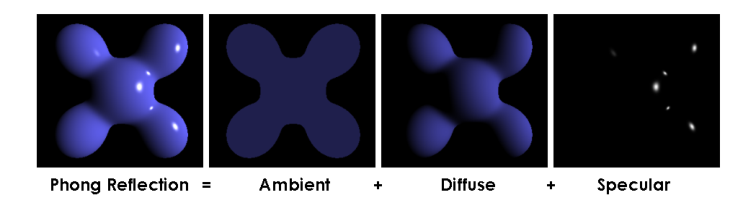
\includegraphics[scale=0.5]{assets/phong_model.png}
\end{center}
\subsubsection{Refraction}

\paragraph{Snell's Law}
\[
\frac{\sin \alpha_1}{\sin \alpha_2} = \frac{c_2}{c_1} = \frac{n_1}{n_2}
\]
where $n_i = \frac{c_{\text{vacuum}}}{c_i}$ is the refractive index.

\paragraph{Huygens' Principle}
Diffraction is caused by wave interference near obstacles.

Each point of a wavefront acts as a source of spherical waves. These elementary waves interfere and form the resulting wave.

\textbf{Intuition:}
At openings (e.g., slits), waves spread out and become circular. With multiple slits (gratings), interference creates maxima and minima.

\section{Lens Optics}

\subsection{Lens Types}
Convex, concave, and combinations (convex-concave, etc.).

\subsection{How Lenses Work}
Lenses bend light via refraction ($c_{\text{air}} > c_{\text{glass}}$):
\begin{itemize}
  \item Convex lens: converges parallel rays
  \item Concave lens: diverges rays
\end{itemize}

\subsection{Ideal Convex Lens}
\begin{itemize}
  \item Parallel rays converge at focal point $F$ (focal length $f$)
  \item Rays through the center are not bent
  \item Rays from $-F$ leave parallel
  \item Rays from $-2F$ focus at $2F$
\end{itemize}

Focal point = Brennpunkt, \quad Focal length = Brennweite

\subsubsection{Lens Formula}
\[
\frac{1}{f} = \frac{1}{s} + \frac{1}{s'}, 
\quad 
\frac{h}{s} = \frac{h'}{s'}
\]

\subsubsection{Image Formation}
\begin{itemize}
  \item $s > 2f$: image between $F$ and $2F$
  \item $f < s < 2f$: image beyond $2F$
  \item $s < f$: virtual image behind the observer
\end{itemize}

\subsection{Aberrations}
Real lenses don't behive like the ideal ones.
\subsubsection{Spherical Aberration}
Bispherican convex lenses wor only work well for beams close to the axis. The focal length varies for beams far away from the axis.
Fixed using aspherical lenses (more expensive).

\subsubsection{Chromatic Aberration}
Different wavelengths focus at different points due to dispersion.  
Fixed using achromatic lens combinations.

\subsection{Multiple Lens Systems}
Used to compensate for aberrations.  
Objective lenses typically use 3-15 elements.

\section{Camera Models}

\subsection{Pinhole Camera}
Projects objects through a small hole.

Tradeoff:
\begin{itemize}
  \item Smaller hole $\Rightarrow$ sharper image
  \item But less brightness
\end{itemize}

Image forms a blur spot called the \textit{circle of confusion}.

Solution: use a lens.

\subsection{Camera with Lens}
Use a lens allows sharper images. Image is captured by a sensor. Incorrect focus leads to blur.

\subsection{Classification by Focal Length}
To obtain a natural perspective, focal length $\approx$ image diagonal.

Example: $24 \times 36\,\text{mm}$ film $\Rightarrow$ diagonal $\approx 43\,\text{mm}$  
$\Rightarrow$ normal focal length $\approx 50\,\text{mm}$

\begin{itemize}
  \item Short focal length: wide-angle lens
  \item Long focal length: telephoto lens
\end{itemize}

\subsection{Cropping vs.\ Background Magnification}
\begin{itemize}
  \item Increasing focal length alone $\Rightarrow$ cropping effect
  \item Changing both position and focal length $\Rightarrow$ background magnification while keeping subject size constant
\end{itemize}
\section{Image Sensors}

\subsection{Analog Photography}
These photos were done with \textbf{Photochemical processes}, that worked in three steps
\begin{enumerate}
  \item Film Emulsion: The film contained grains of \textbf{silver halides}. When a photon hit this grain, the halide would turn into \textbf{metallic silver}.
  
  \item Development: The remaining halides are washed away, making a \textbf{negative image}. The sections hit with light were dark because of the silver.
  
  \item Photo creation: Conversion to positive image by another photographic emulsion using the negative. 
\end{enumerate}

\subsection{Digital Photography}
Nowadays we directly detect the photons.

\begin{itemize}
  \item A photon absorbed in a semiconductor, pushes electrons from their places (orbit change). This leads to \textbf{Electron-hole pairs}
  
  \item To make the pairs usable, the charges must be separated. Done by an electric field which results in a \textbf{photocurrent}
  
  \item The more photons are set free, the higher the current measured. Is mostly linear, with some loss in linearity at really high intensities.  
\end{itemize}

\subsubsection{Sensor Types}
\begin{itemize}
  \item Metal-Oxide Semiconductors (MOS): Charges are stored in a 'trap' formed by isolating metal oxide.
  
  This format is used in \textbf{Charged Couple Devices} (CCD Sensors). One MOS element for each pixel.

  The read out is done sequentially at the end, by moving the lines downwards and to the right. The diagramm of how the move is quite interesting and in the presentation. 
  Basically done using electric fields to 'adjust' the trap to the next cell

  \begin{center}
    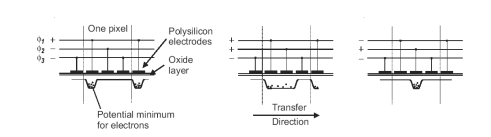
\includegraphics[scale=0.7]{assets/ccd_sensor.png}  
  \end{center}
  
  \item \textbf{Active Pixel Sensors} integrate CMOS. Which is a MOS with some extra electronics for each pixel. This is done to, for example, amplify the charge 

  Readout can be done independently, without moving (which makes things easier)

  \item \textbf{High Dynamic Range Sensors (HDR Sensor)}. Handle non-linear responses (e.g a person behind a light source ).Logarithmic response

  Used for High Dynamic Range CMOS (HDRC) sensors

  Example: Imagine light source triggers a light level of $10^6$, and the person a value of $50$, with variations for each feature.
  
  So because the linear mapping is in range $[0,255]$, all variations of the face will basically map to 0. 
  
  The solution for this could be a non-linear mapping: a \textbf{Logarithmic mapping} will handle a lot of this.
\end{itemize}

\subsubsection{Color Arrays}
Each MOS element can only access information from one color (using a filter). So what is usually done
is an array of arrangement for each filter.

\textbf{Bayer Pattern:}
\begin{center}
  \begin{tabular}{|c|c|}
    \hline
    green & red \\
    \hline
    blue & green \\
    \hline
  \end{tabular}
\end{center}

This makes it so that a part of the color information is missing. This is called \textbf{mosaicking}

To fix this, \textbf{demosaicking} is used.

%--------------------------------------------------------

\section{Camera and Film parameters}

\begin{itemize}
  \item Image diagonal: Larger sensors suffer less from noise (for fixed pixel number). 
  
  \item Focal Length: Depends on size of film/sensor
  \begin{itemize}
    \item 50mm are normal focus for $36\times 24 mm$ image format ($35mm$ film)
    \item 16mm is normal focus for $13.2\times 8.8mm$ image format ($1$ inch sensor)
    \item Shorter focal length: wide lens
    \item Longer focal length: tele lens
  \end{itemize}
  
  \item Exposure time: $1/1000,1/500,\dots,1/2,1$s
  
  \item Aperture: Measured by $\frac{f}{d} = \frac{\text{focal length}}{\text{Aperture diameter}}$
  
  1 is large, 45 is small.

  \item Sensitivity: Given in ISO scale. ISO 100 is pretty standard, ISO 400 is for high-speed but it can lead to noise.
  
  If you use high sensitivity + low exposure, you can get sharp photos in sports-like environments.
\end{itemize}

%--------------------------------------------------------

\section{Color and Perception}

Essential in computer graphics, image processing, color science\dots

\subsection{Physical Background}

Visible light only ranges from $380$ to $750$nm.

Light (photons) are emmited from photons when outer electrons change their orbits and lose energy.

Light is a really small fration of the electromagnetic spectrum.

This range is so important because it is the main range that passes through the atmosphere, emmited from the sun.

Not all animals percieve the same ranges (insects percieve UV)

The visible spectrum contains seven colors: red, orange, yellow, green, blue, indigo, violet.

Memory Hook: \textbf{Richard Of York Gave Battle In Vain}

\subsection{Biological Background}

Human retina (sensor) has two classes of photo receptors:
\begin{itemize}
  \item 120 million rods: Distributed over retina, multiple rods connect to same nerve.
  \item 6 million cones: Mainly in center of retina. Each cone has its own nerve end.
\end{itemize}

Rods are used mainly for night vision \textbf{scotopic vision}. Poor sharpness, no color perception.

Cones handle daylight vision \textbf{photopic vision}. Low sensitivity, but better sharpness and colors.

Humans can see 40 grayscales, but 2 million colors.

We will focus on daylight vision

\subsubsection{Tricolor Imaging}

Humans have three types of cones (L,M,S), each of them being sensitive 
with different frequency ranges: red, green, blue.

The visual of a color is the combination of the impact on the three cones \textbf{tristimulus values}

The tristimulus value $Q_i$ of a cone of type $i = 1,2,3$ for L-,M-,S- cones is:
\[
Q_i = \int C(\lambda)R_i(\lambda) d\lambda
\]
\textbf{Note: This is a definite integral over the wavelength} 

\begin{itemize}
  \item $\lambda$: Wavelength
  \item $C(\lambda)$ stimulus (product of illuminant and reflectance)
  \item $R_i(\lambda)$ spectral sensitivity of cone $i$
\end{itemize}

\textbf{Rough idea: } For light source C that provides a range of wavelengths, and the existing sensitivity curve R, what is the total
value for this specific cone type over all wavelengths.

\begin{center}
  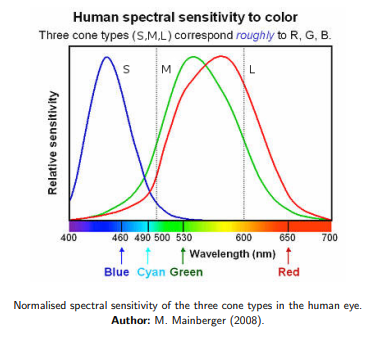
\includegraphics[scale=0.7]{assets/human_spectral_sensitivity.png}  
\end{center}
This is the sensitivity curve.


\paragraph{Metamerism}
Two colors with different spectral composition, can map to the same tristimulus values. \textbf{Metamaric colors} are indistinguishable by humans.

\subsubsection{Color perception in animals}

Mammals used to only have 2 receptors, which was good enough given they lived mostly at night.

35 million years ago monkeys got third receptor, which enabled to distinguish between mature and immature fruits.

Some fish and birds have 4 receptors: Red, green, blue and ultraviolet

Some animals such as shrimps have even more receptors. (up to 12!!) Each eye has trinocular depth perception!

\textbf{Note: } Colours are no objective physical reality. It's just an interpretation of the existing wave length spectrum.

%--------------------------------------------------------

\subsection{Technical color spaces}

\subsubsection{RGB model}

Additive model based on trichromatic vision

\begin{itemize}
  \item Red (1,0,0)
  \item Green (0,1,0)
  \item Blue (0,0,1)
  \item Black (0,0,0)
  \item White (1,1,1)
\end{itemize}

Each color has its complementary where mixing with it gives white.

Imagine it as a cube. In computers, the range $[0,1]^3$ is replaced by the byte range $[0,255]^3$

\subsubsection{CMY Model}

Used by printers that place colors on white paper. Uses cyan, magenta, yellow (complements of RGB)

The model is \textbf{subtractive}, works the opposite of RGB

Example: The toner for yellow actually absorbs blue, so only its complement remains, appearing yellow to the eye.

\[
\begin{pmatrix}
C\\
M \\
Y
\end{pmatrix}
=
\begin{pmatrix}
1\\
1 \\
1
\end{pmatrix}
-
\begin{pmatrix}
R\\
G \\
B
\end{pmatrix}
\]

\subsubsection{CMYK Model}

The one actually used by printers to save toner. K is black. Useful for printers that use a lot of black

Transition is 

\begin{itemize}
  \item $K \leftarrow min(C,M,Y)$
  \item $C \leftarrow C -K$
  \item $M \leftarrow M -K$
  \item $Y \leftarrow Y -K$
\end{itemize}

\subsubsection{HSV Model}

\begin{center}
  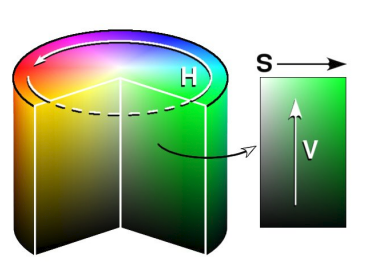
\includegraphics[scale=0.7]{assets/HSV_model.png}  
\end{center}

\begin{itemize}
  \item H: hue - Polar angle in the horizontal plane. 
  \item S: saturation - radius in horizontal plane. 'Colorish' attribute
  \item V: value - vertical axis. How dark/bright a color is
\end{itemize}

It is advanageous when illumination changes appear.

\begin{itemize}
  \item Global multiplicative change $\Rightarrow$ global illumination change (light source). H and S is invariant here
  \item Local multiplicative change $\Rightarrow$ shadow (diffuse reflection). H and S is invariant here.
  \item Local additive change $\Rightarrow$ highlights (specular reflection). H is invariant here.
\end{itemize}

Hue H is undefined for graytones RGB to HSV is slightly complicated

\subsubsection{YCbCr Model}
\label{sec:YCbCr}
Used in television, JPEG and MPEG compression

\begin{itemize}
  \item Y: luma component. Roughly a grayscale of the image
  \item Cb: Chroma component. Deviation from gray in the blue-yellow direction
  \item Cr: Chroma component. Deviation from gray in the red-cyan direction.
\end{itemize}

This model is used because while Y is needed to be preserved at high quality, Cb and Cr can be downsampled without that much of a visual loss. Used in JPEG compression.

Conversions are also tough, but worth to check out.
\section{Degradation in Digital Images}
Two types
\begin{itemize}
  \item Noise
  \item Blur
\end{itemize}
\subsection{Noise}
\begin{itemize}
  \item Common in digital images
  \item Come from bad quality sensor, or specific acquisition methods (ultrasound).
  \item Also can come from the transmission, like interfering channels or wireless transmission.
\end{itemize}

Noise is modelled stochastically.

\subsubsection{Additive Noise}
Most important type. 
\[f_{i,j} = g_{i,j}+n_{i,j}\]
\begin{itemize}
  \item g is the original image
  \item n is the noise
  \item f is the noisy image
\end{itemize}

n may have different distributions

\paragraph{Uniform Noise}: Not too realistic, but easy to simulate

Constant density function within some interval $[a,b]$
\[p(x) = \begin{cases}
  \frac{1}{b-a} \quad x\in [a,b]\\
  0 \quad else
\end{cases}\]

To simulate it in C
\begin{lstlisting}
  U = a + (float)rand() / RAND_MAX * (b - a)
\end{lstlisting}
With (float)rand() generates a uniformly distributed number in $[0,RAND_MAX]$. The division casts
it into a range $[0,1]$

To apply for an image, do $g+U$ for each pixel.

Usually the range $[-a,a]$ (symmetric interval) is used so that the mean of the value of the noisy image stays the same.

\paragraph{Gaussian Noise} The most important, because it can be applied in a lot of real situations.

\[p(x)= \frac{1}{\sigma\sqrt{2\pi}}\exp\left(\frac{-(x-\mu)^2}{2\sigma^2}\right)\]

\begin{center}
  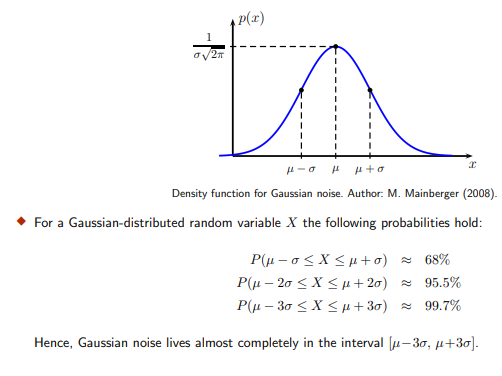
\includegraphics[scale=0.6]{assets/gaussiannoise.png}  
\end{center}

To generate Gaussian Noise we use the \textbf{Box-Mueller algorithm}

\begin{lstlisting}
  // These are the uniformly distributed random varialbes U,V
  U = (float)rand() / RAND_MAX;
  V = (float)rand() / RAND_MAX
\end{lstlisting}

And then we define
\[N = \sqrt{-2\ln U}\cos(2\pi V)\]
\[M = \sqrt{-2\ln U}\sin(2\pi V)\]

And they are independent random variables with \textbf{Normal distribution}
(we currently only need one of the two variables but I think they had some usecase)

So to degrade gray image f with additive Gaussian noise with mean $\mu = 0$ and standard deviation $\sigma$ we replace f with
\[f + (\mu + \sigma N) = f + \sigma N\]

\textbf{WARNING:} Careful when adding noise to handle when it leaves the color range interval $[0,255]$.


\subsubsection{Multiplicative Noise}
New format
\[f_{i,j} = g_{i,j} + n_{i,j}g_{i,j} = (1+n_{i,j})g_{i,j}\]

\subsection{Impulse Noise}
Unlike multiplicative or additive, degrades the image at \textbf{some} pixels where erroneous gray values are created.

\begin{itemize}
  \item Unipolar noise: Gives degradaion by only having one gray value
  \item \label{itm:salt-pepper-noise} Bipolar noise: Gives degradation by two gray values. Some are replaced by one value, some by other. Bipolar noise with highest-lowest gray values is called \textbf{salt-and-pepper} noise.
\end{itemize}

\subsubsection{Measuring Noise}
\paragraph{Image statistics}: Let $g$ be the initial image with $M\times N$ pixels

Its mean (average gray value) is
\[\mu(g) := \frac{1}{MN}\sum_{i=1}^{M}\sum_{j=1}^{N}g_{i,j}\]

The variance 
\[\sigma^2(g) := \frac{1}{MN}\sum_{i=1}^{M}\sum_{j=1}^{N}(g_{i,j} - \mu)^2\]

The standard deviation
\[\sigma(g) = \sqrt{\sigma^2(g)}\]

\paragraph{Error Measures}: Let f be a noisy version of g

Mean Squared Error (MSE) between f and g
\[MSE(f,g) := \frac{1}{MN}\sum_{i=1}^{M}\sum_{j=1}^{N}(f_{i,j} - g_{i,j} )^2\]
The smaller the better

Peak-signal-to-noise ratio (PSNR). For a maximum gray value of 255
\[PSNR(f,g) := 10\log_{10}\left(\frac{255^2}{MSE(f,g)}\right)\]
Unit is in decibel (dB). Higher the better. Values $\geq 30$dB, noise is barely visible.

\subsection{Blur}
Caused by defocusing, atmospheric disturbance, or motion during image acquisition.

For simplicity, let's assume identical blurring effect for everything.

Can be roughly defined as the weighted average of the gray values in a neighborhood.

This weighted averaging is called \textbf{convolution}

\subsubsection{Convolution}

\paragraph{Discrete Convolution} Given two 1-D signals $g = (g_i)_{i\in\mathbb{Z}}$ and $w = (w_i)_{i\in\mathbb{Z}}$. 

\[(g \ast w)_i := \sum_{k\in\mathbb{Z}}g_{i-k}w_k = \sum_{m\in\mathbb{Z}}g_m w_{i-m}\text{ with } m=i-k\]

The entries of w can be regarded as \textbf{mirrored} weights for averaging the components of g

Example: $g = [4,2,6,4,0,2]$ and $w = [2/5,2/5,1/5]$

$w$ is called the \textbf{convolution kernel} and the weights is the mirrored version

so for pixel in g at index 1 (value 2). The new value would be
\[g_1 = 1/5\cdot 4 + 2/5\cdot 2 + 1/5 \cdot 6\]
\textbf{Note the mirroring}

\paragraph{Continous Convolution} of two 1-D signals $g,w: \mathbb{R} \to \mathbb{R}$

\[(g\ast w)(x) := \int_{\mathbb{R}}g(x-x')w(x')dx'\]

\paragraph{Example} Lets say $g_i$ is the value of the stock market at day $i$.

We want the average of the last 200 days

We define the convolution kernel as
\[w_k := \begin{cases}
  \frac{1}{200} \quad \text{for } k = 0,\dots,199\\
  0 \quad \text{else}
\end{cases}\]
\textbf{Note that it says 0-199 because the convolution kernel is the non-mirrored version}

So then
\[f_i = \sum_{k \in\mathbb{Z}}g_{i-k}w_k = \frac{1}{200}\sum_{k=0}^{199}g_{i-k}\]


\paragraph{Two-Dimensional Discrete convolution}
Given two images $g = (g_{i,j})_{i,j\in\mathbb{Z}}$,$w = (w_{i,j})_{i,j\in\mathbb{Z}}$

\[(g\ast w)_{i,j} := \sum_{k\in\mathbb{Z}}\sum_{l\in\mathbb{Z}}g_{i-k,j-l}w_{l,k}\]

\paragraph{Two-Dimensional continous convolution}
Given two images $g,w : \mathbb{R}^2 \to \mathbb{R}$

\[(g\ast w)(x,y) := \int_{\mathbb{R}}\int_{\mathbb{R}}g(x-x',y-y')w(x',y')dx'dy'\]

\subsubsection{Modelling Blur by convolutions}
\begin{itemize}
  \item Defocussed Optical System: Uniform distribution but cylinder-shaped
  \begin{center}
    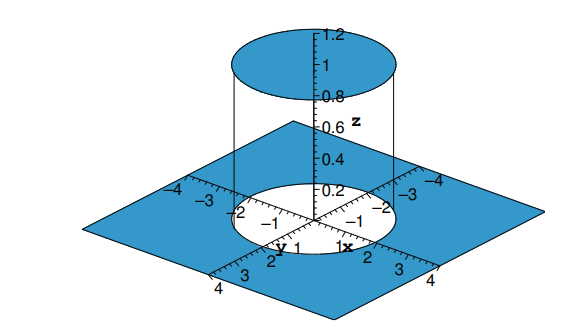
\includegraphics[scale=0.4]{assets/defocussed_optical_system.png}  
  \end{center}
  
  \item Atmospheric Disturbance: Approximated to 2-D gaussian
  
  \begin{center}
    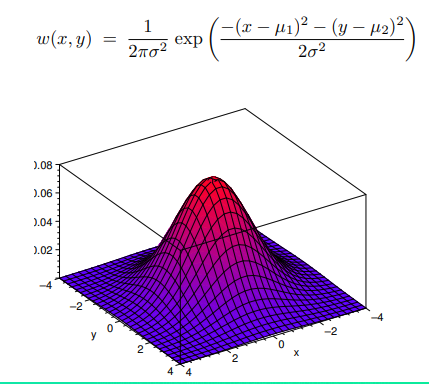
\includegraphics[scale=0.4]{assets/atmospheric_disturbance.png}  
  \end{center}
  
  \item Motion Blur: 1-D box function along the direction of motion
  
  \begin{center}
    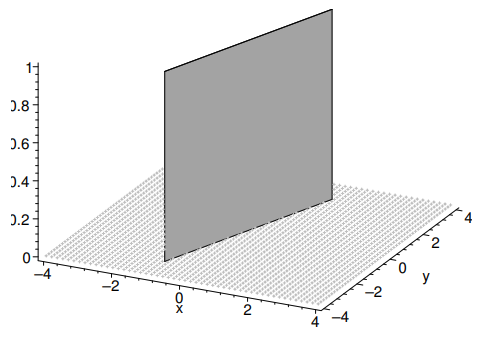
\includegraphics[scale=0.4]{assets/motion_blur.png}  
  \end{center}
  
\end{itemize}

\subsection{Combining Blur and Noise}
A frequently used degradation model of some initial image g with a shift-invariant blurring kernel w and
additive noise n is given by

\[f = g\ast w + n\]
First the object is blurred and then the noise is added

\subsection{Sources of image degradation}
\begin{itemize}
  \item Motion Blur
  \item Aberrations: Imperfections of camera optics
  \item Defocussing: Disk-shaped blur 
  \item Grain: Physical limitation of photographic film
  \item Mosaicking: Bayer pattern, problem for digital color sensors
  \item Quantum Noise: Physical perturbation in CCD Sensors
\end{itemize}
\section{Image Transformations}
Idea is to represent a signal as a linear decomposition of basic (trigonometric) functions.

These transformations are used to make certain features of a feature more explicit.

Images are just 2D signals, so same ideas can be used here.

\subsection{Complex Numbers}
Its a set $\mathbb{C}$ that extends $\mathbb{R}$ so that you can compute the square root of a negative number.

It consists of $z = a+bi \in \mathbb{C}$ with a real part $Re(z) = a \in \mathbb{R}$ and an imaginary part $Im(z) := b \in \mathbb{R}$.

The \textbf{conjugate complex number} of $z = a+bi$ is $ \overline{z} = a-bi$

It can also be represented as the vector $(a,b)^T \in \mathbb{R} ^2$

\subsubsection{Operations on complex numbers}
Usual operations, for division you multiply with conjugate for nicer numbers.

The \textbf{norm} is
\[|z| := \sqrt{z\overline{z}} = \sqrt{a^2 + b^2}\]

\subsubsection{Euler's Formula}
We already know the following power series representations
\[e^x = \sum_{k=0}^{\infty}\frac{x^k}{k!}, \quad \cos x = \sum_{k=0}^{\infty}(-1)^k\frac{x^{2k}}{(2k)!}, \quad \sin x = \sum_{k=0}^{\infty}(-1)^k \frac{x^{2k+1}}{(2k+1)!}\]

So we can derive to the following formula
\[e^{i\phi} = \sum_{k=0}^{\infty}\frac{(i\phi)^k}{k!} = \sum_{k=0}^{\infty}\frac{(i\phi)^2k}{(2k)!} + \sum_{k=0}^{\infty}\frac{(i\phi)^{2k+1}}{(2k+1)!}=\]
\[=\sum_{k=0}^{\infty}(i^2)^k\frac{(\phi)^2k}{(2k)!} + \sum_{k=0}^{\infty}i(i^2)^k\frac{(\phi)^{2k+1}}{(2k+1)!}=\]
\[=\sum_{k=0}^{\infty}(-1)^k\frac{(\phi)^2k}{(2k)!} + i\sum_{k=0}^{\infty}(-1)^k\frac{(\phi)^{2k+1}}{(2k+1)!}=\]
\[= \cos \phi + i\sin \phi\]

And we can compute
\[|e^{i\phi}| = \sqrt{\cos^2 \phi + \sin^2\phi} = 1\]

It also has $2\pi$ \textbf{periodicity}

And knowing that $\sin-\phi = -\sin\phi$ and that $\cos-\phi = \cos\phi$ we can compute the following helper functions
\[\cos\phi = \frac{e^{i\phi} + e^{-i\phi}}{2} ,\quad \sin\phi = \frac{e^{i\phi} - e^{-i\phi}}{2i}\]

Following all these formulas, we arrive at the \textbf{polar form}
\[z = a+bi = re^{i\phi}\]
with $r = |z|$ (radius) and angle
\[\phi := arg(z) := \begin{cases}
  \arccos (\frac{a}{r}) \quad \text{ if } b \geq 0\\
  -\arccos (\frac{a}{r}) \quad \text{ if } b < r
\end{cases} \in (-\pi,\pi]\]

This can be useful for multiplication
\[z_1z_2 = |z_1||z_2|e^{i(\phi_1 + \phi_2)}\]


\subsection{Linear Algebra Prerequisites}
\subsubsection{Vectors and basis}
To represent vector $f\in\mathbb{R}^N$ with a basis $\{b_1,\dots,b_N\}$ of $\mathbb{R}^N$

\[f = \sum_{i=1}^{N}\langle f,b_i \rangle b_i\]

Where $\langle .,. \rangle$ is the Euclidean scalar product $\sum_{i=1}^{N}f_i\cdot g_i$

This coefficient $\langle f,b_i \rangle$ is the projection of f onto basis vector $b_i$

For vectors $f\in\mathbb{C}$ you use the Hermitian inner product
\[\langle f,g \rangle := \sum_{i=1}^{N}f_i\overline{g}_i\]

Note: Is it still symmetric? (for my own curiosity)
\[\langle f,g \rangle = \sum_{i=1}^{N}f_i\overline{g}_i = \sum_{i=1}^{N}(a_i + ib_i)(a'_i - ib'_i) = \sum_{i=1}^{N}(a_ia'_i - ia_ib'_i + ia'_ib_i - i^2b_ib'_i) = \]
\[\sum_{i=1}^{N}(a_ia'_i - ia_ib'_i + ia'_ib_i + b_ib'_i) =  \overline{\langle g,f \rangle}\]

\textbf{NOT SYMMETRIC!!}


This is fine for discrete values and vectors, but we usually want continous cases.

\subsubsection{Continous vectors}
A function $f:\mathbb{R}\to\mathbb{R}$ can be regarded as 'infinite dimensional vector'

So for an infinite set of orthonormal basis functions $\{b_u | u\in\mathbb{R}\}$

\[f = \int_\mathbb{R} \langle f,b_u\rangle b_u\]
With the inner product 
\[\langle f,g \rangle := \int_\mathbb{R}f(x)g(x)dx\]

And for complex functions $f:\mathbb{C}\to\mathbb{C}$. We have to also use the conjugate

\[\langle f,g \rangle := \int_\mathbb{C}f(x)\overline{g}(x)dx\]

Same thing, just continous.
\subsection{Continous Fourier Transform in 1D}
We want decompose a signal into its frequency components


Fourier transform for a 1-D function $f:\mathbb{R}\to\mathbb{R}$ is defined as
\[\tilde{f}(u) := \mathcal{F}[f](u) := \int_{-\infty}^\infty f(x)e^{-i2\pi u x}dx\]
Where $\hat{f}(u)$ is the coefficient of $f$ with respect to the inner product

with the basis function $g_u(x) = e^{i2\pi u x}$, so the conjugate changes the symbol.

Because of Eulers formula, we can regard
\begin{itemize}
  \item $Re(\hat{f}(u))$ as the component of f in regard to $\cos (2\pi u x)$
  \item $Im(\hat{f}(u))$ as the component of f in respect to $\sin(2\pi u x)$
\end{itemize}

So in general $\{\hat{f}(u) | u \in \mathbb{R}\}$ is a representation of the function $\{f(x) | x \in \mathbb{R}\}$ in the frequency domain. This is called \textbf{Fourier Domain}
\subsubsection{Inverse 1-D Fourier Transform}
\[f(x)= \mathcal{F}^{-1}[\hat{f}](x) := \int_{-\infty}^{\infty}\hat{f}(u)e^{i2\pi u x}du\]

So one is a forward transform, the other is a backward transform, given that
\[\hat{f}(u) = \langle f,g_u\rangle\]
and
\[f(x) = \int_{-\infty}^{\infty}\langle f,g_u\rangle g_u du\]

Usually, the polar form of $\hat{f}(u)$ is used.
\begin{itemize}
  \item $|\hat{f}(u)|$ i called the Fourier spectrum. The power spectrum is just $|\hat{f}(u)|^2$, and they describe the importance of frequency u within signal f.
  \item $arg(\hat{f}(u))$ is called the phase angle
\end{itemize}
\subsubsection{Example: Fourier Transform of box function}

\begin{center}
  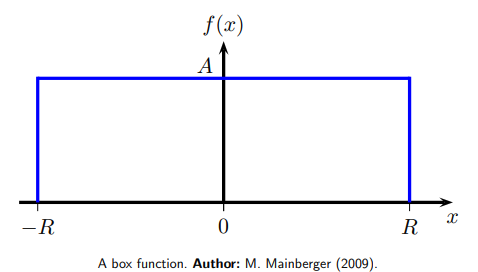
\includegraphics[scale=0.5]{assets/box_function_fourier_transform.png}
\end{center}

\begin{center}
  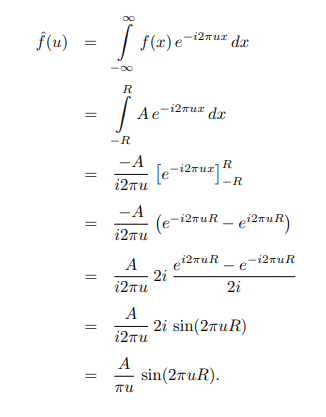
\includegraphics[scale=0.8]{assets/box_function_fourier_transform_formula.png}
\end{center}

So now to compute the spectrum
\[|\hat{f}(u)| = \left| \frac{A}{\pi u} \right| |\sin (2\pi u R)| = |2RA| \left|\frac{\sin(2\pi u R)}{2\pi u R}\right| = 2RA |sinc (2\pi u R)|\]
With \textbf{sinc} $:= \frac{sin(x)}{x}$

So we can see that $|\hat{f}(0)| = 2RA$ and it becomes 0 in $u = \frac{k}{2R}$ wiwth $k \in \mathbb{Z} \backslash \{0\}$
\begin{center}
  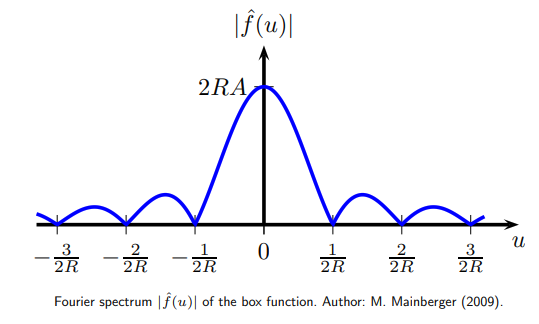
\includegraphics[scale=0.7]{assets/box_function_fourier_transform_result.png}
\end{center}

Given that the box function has points with infinitely high derivative, you need trigonometric functions with infinitely high frequency to be able to represent that.

\subsection{Continous Fourier Transform in 2D}
\[\hat{f}(u,v) := \mathcal{F}[f](u,v) \int_{-\infty}^{\infty}\int_{-\infty}^{\infty} f(x,y)e^{-i2\pi (ux +vy)}dx dy\]
And the inverse of it being
\[f(x,y) := \mathcal{F}^{-1}[f](u,v) \int_{-\infty}^{\infty}\int_{-\infty}^{\infty} \hat{f}(u,v)e^{i2\pi (ux +vy)}du dv\]

\textbf{Note:} So, there seems to be an inverse paralelism between the compactness of a function and the size of the output of the Fourier Transform
\subsection{Higher Dimensions}
It just continues growing as usual. This means that the Fourier Transform is \textbf{separable}. An m-dimensional transform can be a computed with a sequence of m one-dimensional transforms.

\subsection{Properties of Fourier Transforms}
\begin{itemize}
  \item Linearity: $\mathcal{F}[af + bg] = a\mathcal{F}[f] + b\mathcal{F}[g]$
  \item Similarity Theorem $\mathcal{F}[f(ax,by)](u,v) = \frac{1}{|ab|}\mathcal{F}[f](\frac{u}{a},\frac{v}{b})$ This is what is mentioned above, stretching in the spatial domain gives in to shortening of the fourier domain. Inversely proportional in scale to some extent.
  \item Differentiation: 
  \[\mathcal{F}\left[\frac{\partial^{n+m}f}{\partial x^n\partial y^m}\right] (i2\pi u)^n(i2\pi v)^m \mathcal{F}[f](u,v)\]
  Differentiation in the spatial domain gives to multiplication in the fourier domain
  \item Shift Theorem
  \[\mathcal{F}[f(x-x_0,y-y_0)](u,v) = e^{-i2\pi(ux_0 + vy_0)}\mathcal{F}[f](u,v)\]
  Shift in spatial domain rotates phase angle in Fourier Domain. The Fourier Spectrum is \textbf{NOT} affected
  \item Rotation Invariance: Rotation of an image maps to the same rotation in the Fourier Transform
  \item Convolution Theorem 
  \[\mathcal{F}[f \ast g] = \mathcal{F}[f]\cdot \mathcal{F}[g]\]
  Convolution is multiplication in the fourier domain.

  So we can compute
  \[f\ast g = \mathcal{F}^{-1}[\mathcal{F}[f]\cdot\mathcal{F}[g]]\]
  \item Product of two functions: Literally the inverse of the convolution theorem
  \[\mathcal{F}[f\times g] = \mathcal{F}[f] \ast \mathcal{F}[g]\]
  \item Fourier Transform of a Gaussian: Gaussian functions stay similar under the FT
  \[f(x,y) := \frac{1}{2\pi\sigma^2}\exp\left(\frac{-(x^2+y^2)}{2\sigma^2}\right) \Rightarrow \hat{f}(u,v) = \exp\left(\frac{-(2\pi)^2(u^2+v^2)}{2\sigma^{-2}}\right)\]

  So it remains a gaussian with just  different parameters to some extent

  \item Fourier Transform of Delta Comb: A \textbf{delta pulse} $\delta$ is a model for an infinitely sharp centered in 0.

  The integral of a function f times a delta pulse $\delta$ evaluates f in 0,
  \[\int_{-\infty}^{\infty}f(x)\delta(x)dx = f(0)\]

  We can also shift the delta pulse $\delta(x-x_0)$
  \[\int_{-\infty}^{\infty}f(x)\delta(x-x_0)dx = f(x_0)\]

  A \textbf{delta comb} is then a sequence of delta pulses, shaped like a comb.
  The FT of a delta comb with peak distance $\lambda$ (distance between peaks) is another delta comb with peak distance $\frac{1}{\lambda}$
  \[g(x) = \sum_{k=-\infty}^{\infty}\delta(x-k\lambda) \Rightarrow \hat{g}(u) = \sum_{k=-\infty}^{\infty}\delta\left(u - \frac{k}{\lambda}\right)\]
\end{itemize}

\subsection{Discrete Fourier Transform}
So far everything was continous, which isn't realistic for images and such. Even with 1D signals, we only get a sample, not the infinite wave.

\subsubsection{Sampling Theorem}
If you sample high-frequency signals too coarsely, low-frequency artifacts arise

\begin{center}
  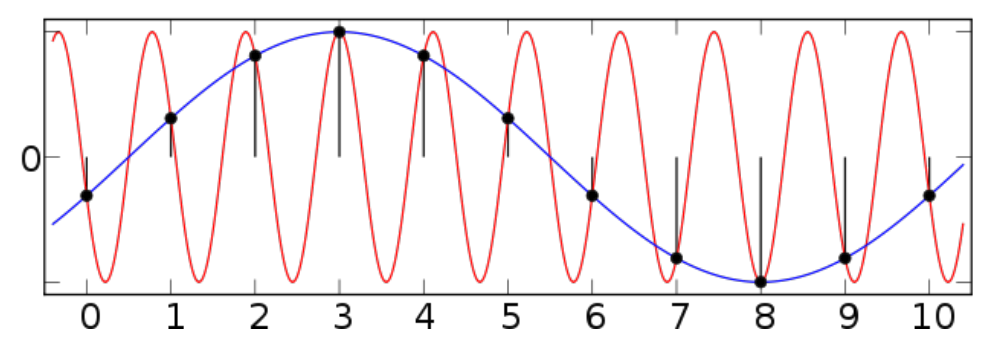
\includegraphics[scale=0.5]{assets/aliasing.png}
\end{center}
This is called \textbf{aliasing}. Also happens when downscaling images incorrectly.

\begin{center}
  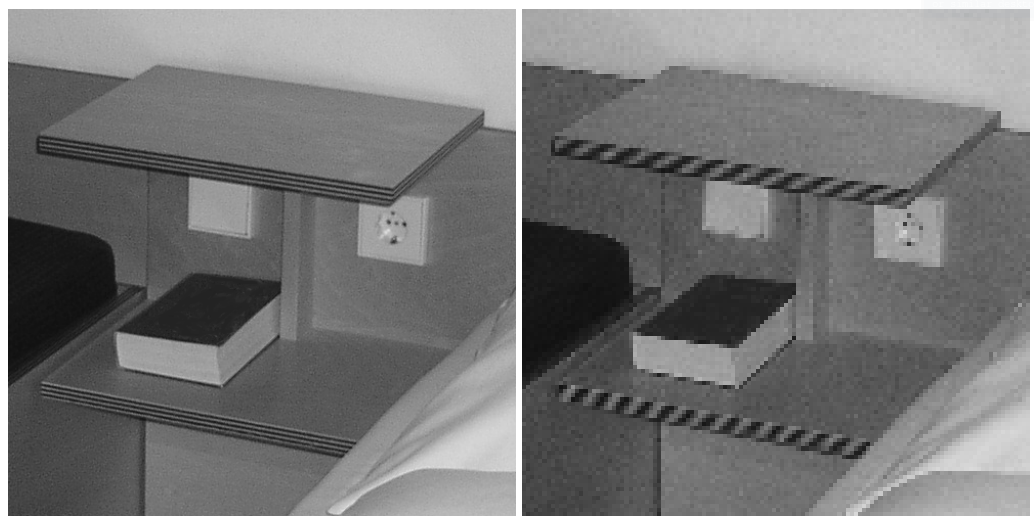
\includegraphics[scale=0.5]{assets/aliasing2.png}
\end{center}
This happened because to downscale by a scale of 4, we just took every fourth pixel.

So the sampling theorem is: Let signal $f$ be \textbf{band-limited}. This means there exists a bound $W$ on frequencies
\[\hat{f}(u) = 0 \quad |u| > W\]

So the theorem says, to sample a band-limited signal without aliasing artifacts, you have to sample the highest frequency more than twice per period.

So the sampling distance $h$ should be
\[h < h_{max} := \frac{1}{2W}\]
\paragraph{Example: Clock} The clock hand in charge of the seconds has a $W = \frac{1}{60}Hz$

So according to the theorem
\[h < h_{max} = 30s\]
\begin{itemize}
  \item For $h = 15s$, each sampling is a quarter turn, pretty accurate
  \item For $h = 30s$, each sample is half a turn, so we are unable to know if it's going forward or backward. Not good anymore
  \item For $h = 45s$,  each sample is quarter turn in the other direction. Seems to go backwards. Doesn't work.
\end{itemize}
So with too coarse sampling, you misinterpret data. A very clear example of this is car tires when they go fast, your eye doesn't match the necessary refresh rate. \textbf{COOL!}

The critical sampling frequency $2W$ is called the \textbf{Nyquist frequency}

The cool thing about this is, if we stand by this theorem and its rules, we can reconstruct the signal from the samples.

\paragraph{Whittaker Interpolation Formula: }
\[f(x) = \sum_{k= -\infty}^{\infty}f(kh) sinc \left(\frac{\pi}{h}(x-kh)\right)\]
For now it's a mistery the reasoning behind the formula, will be cleared up later.

\paragraph{Note: }The theorem has to be held in all dimensions for it to work

\paragraph{Visually explained aliasing effect: } Explanation below

\begin{center}
  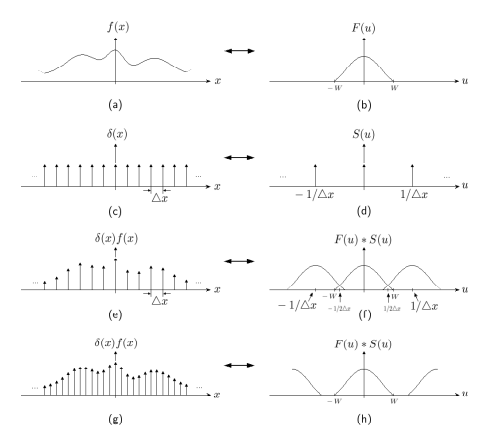
\includegraphics[scale=0.7]{assets/sampling_theorem.png}
\end{center}
\begin{itemize}
  \item (a): Our function
  \item (b): Its fourier domain, as we can see, it is band limited.
  \item (c): Delta comb with grid distance $\Delta x$
  \item (d): FT of the delta comb, with reciprocal grid distance $\frac{1}{\Delta x}$
  \item (e): Sampling the function using our comb.
  \item (f): The convolution of (b) and (d) gives some overlap, this is the \textbf{aliasing}. The solution from the theorem is to reduce $\Delta x$
  \item (g): Comb with lower $\Delta x$
  \item (g): Because the comb and its FT are inverse, reducing in $\Delta x$ in $\delta$ increases in its FT. This removes the overlap, fixing the aliasing. Now we can reconstruct the signal without artifacts. So the $2W$ arises so that the width between periodic artifacts in the Fourier Spectrum is so big so that they dont overlap. 
\end{itemize}
Given that we know the width of the Fourier Domain $2W$, if we space the signals by more than $2W$, the separation is perfect.

So to restore the signal, we multiply by the box signal of width of $2W$. This is in the fourier domain, in the discrete domain, a box function is a $sinc$ function.

\[f \ast \text{sinc function} = \text{periodical fourier domain function} \cdot \text{box function} \]

\paragraph{Alternatives}: If you can't increase a sufficiently high sampling rate, we can also trim down the highest frequencies so that the requirement is lower. This is done by smoothing the image (e.g Gaussian Convolution) \textbf{before} doing the downsampling
The effect of trimming the higher frequencies can also be imagined visually.

\subsubsection{Discrete Fourier Transform in 1-D}
Goal: Decompose M real values into M complex frequency components

\paragraph{Definition: } The DFT of signal $f = (f_0,\dots,f_{M-1})^T$ is given by
\[\hat{f}_p := \frac{1}{\sqrt{M}}\sum_{m = 0}^{M-1}f_m \exp\left(-\frac{i2\pi pm}{M}\right) \quad (p = 0,\dots,M-1)\]

So $\hat{f}_p = a$ means that frequency p contributes a to the signal.

\paragraph{Inverse: } The IDFT is defined as
\[f_m := \frac{1}{\sqrt{M}}\sum_{p = 0}^{M-1}\hat{f}_p \exp\left(\frac{i2\pi pm}{M}\right) \quad (m = 0,\dots,M-1)\]

\paragraph{Note: } The $\frac{1}{\sqrt{M}}$ factor helps to convert it to an orthonormal basis function. The disatvantage is that it scales multiplication in the fourier domain

\subsubsection{DFT in 2D}
Given image $f = (f_{m,n})$ with $m = 0,\dots,M-1$ and $n = 0,\dots,N-1$:
\[
  \hat{f}_{p,q} := \frac{1}{\sqrt{MN}}
  \sum_{m=0}^{M-1}\sum_{n=0}^{N-1}
  f_{m,n}
  \exp\!\left(-\frac{i2\pi pm}{M}\right)
  \exp\!\left(-\frac{i2\pi qn}{N}\right)
\]
The inverse is derived analogously.

% ----------------------------------------------------------------
\subsubsection{Properties of DFT}
Most properties of the continuous FT carry over:
\begin{itemize}
  \item Linearity
  \item Shift Theorem
  \item Convolution Theorem
\end{itemize}
Properties like the scaling theorem and rotation invariance can only be
approximated on a discrete grid.

\paragraph{Centering the Fourier Spectrum:}
In the raw DFT output, the DC component (lowest frequency) sits at corner $(0,0)$
and high frequencies cluster near $(M/2, N/2)$. We prefer low frequencies in the
center for visualization.

Fix: shift the origin to $(M/2, N/2)$ using the discrete shift theorem with
$p_0 = M/2$, $q_0 = N/2$:
\[
  f_{m,n}
  \exp\!\left(\frac{i2\pi (M/2)\,m}{M}\right)
  \exp\!\left(\frac{i2\pi (N/2)\,n}{N}\right)
  = f_{m,n}\,e^{i\pi(m+n)}
  = f_{m,n}\,(-1)^{m+n}
\]
So simply multiply by a checkerboard of $+1$ and $-1$.

\paragraph{Logarithmic Scaling:}
The DFT output spans many orders of magnitude, so log scaling helps visualization:
\[
  D_{p,q} = c\log\!\left(1 + |\hat{f}_{p,q}|\right)
\]
Choose $c$ so that $\max_{p,q} D_{p,q} = 255$:
\[
  c = \frac{255}{\log\!\left(1 + \max_{p,q}|\hat{f}_{p,q}|\right)}
\]
This maps all values into $[0, 255]$.

\paragraph{Boundary Artifacts:}
Two problems arise from going discrete:
\begin{enumerate}
  \item \textbf{Aliasing} (from the sampling theorem): the spectrum repeats,
        causing aliasing when undersampled.
  \item \textbf{Periodic assumption}: the DFT treats the signal as if it repeats
        infinitely. A signal like $y = x$ gets copy-pasted left-to-right, creating
        sharp jumps at the boundaries. These jumps pollute the spectrum and cause
        \textbf{wraparound errors} in convolution:
        \[
          \hat{f}_{p,q} = \hat{f}_{p+kM,\,q+lN} \quad (k,l \in \mathbb{Z})
          \qquad
          f_{m,n} = f_{m+kM,\,n+lN} \quad (k,l \in \mathbb{Z})
        \]
\end{enumerate}

\textbf{Handling wraparound errors:}
\begin{itemize}
  \item \textbf{Fatalism:} Do nothing; only trust results far from boundaries.
  \item \textbf{Zero Padding:} Add a border of zeros so the convolution kernel
        does not reach across the real boundary. Drawback: zeros can still
        distort the signal.
  \item \textbf{Mirror Padding:} Reflect the image at each boundary.
        Cleanest solution — removes the jump discontinuity entirely — but
        doubles the signal length in each dimension (computationally expensive).
        \begin{center}
          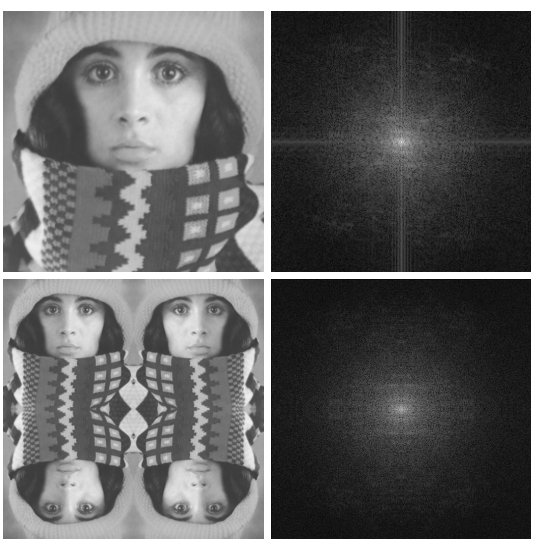
\includegraphics[scale=0.5]{assets/wraparound-error-mirror.png}\\
          Mirroring removes boundary artifacts.
        \end{center}
\end{itemize}

% ----------------------------------------------------------------
\subsection{Fast Fourier Transform (FFT)}
The 1D DFT of a signal of size $M$ costs:
\begin{itemize}
  \item $M^2$ complex multiplications
  \item $M^2 - M$ complex additions
\end{itemize}

\textbf{Idea — divide and conquer:}
\begin{enumerate}
  \item Split the size-$M$ problem into two size-$M/2$ subproblems.
  \item Recurse until size 1.
\end{enumerate}
This gives $\mathcal{O}(M \log_2 M)$ in 1D (and analogously in higher dimensions).

\textbf{Requirement:} $M = 2^k$. Extensions exist for other small prime factors
(3, 5, \dots), covering most non-prime sizes.

\paragraph{Inverse FFT:}
No separate algorithm is needed. To compute the IDFT of $\hat{f}$:
\begin{enumerate}
  \item Conjugate the input: $\overline{\hat{f}_p}$
  \item Apply the forward FFT
  \item Conjugate the result
\end{enumerate}
This works because conjugating flips the sign of the exponent, turning
$e^{-i2\pi pm/M}$ into $e^{+i2\pi pm/M}$, which is exactly the IDFT kernel.

% ----------------------------------------------------------------
\subsection{Discrete Cosine Transform (DCT)}
DFT has two drawbacks:
\begin{itemize}
  \item Complex-valued computations
  \item A local structure (e.g.\ a single jump) affects \emph{all} Fourier
        coefficients globally
\end{itemize}
The DCT and Image Pyramids (next section) each address these issues.

\subsubsection{Definition of DCT}
\textbf{Note:} The DCT is an orthogonal transform with \textbf{real-valued} coefficients.

For a 1D signal $f = (f_0,\dots,f_{M-1})^T$:
\[
  \tilde{f}_p
  := \sum_{m=0}^{M-1} f_m\, c_p \cos\!\left(\frac{\pi(2m+1)p}{2M}\right)
  \quad (p = 0,\dots,M-1)
\]
with $c_0 := \sqrt{\tfrac{1}{M}}$ and $c_p := \sqrt{\tfrac{2}{M}}$ for $p > 0$.

The inverse (IDCT) is:
\[
  f_m
  := \sum_{p=0}^{M-1} \tilde{f}_p\, c_p \cos\!\left(\frac{\pi(2m+1)p}{2M}\right)
  \quad (m = 0,\dots,M-1)
\]
\textbf{Intuition:} We project the signal onto a basis of cosine waves at different
frequencies and record how much of each basis is present.

\textbf{Key advantage over DFT:} The DCT implicitly mirrors the signal at its
boundaries (rather than repeating it), so there are no jump discontinuities and
boundary artifacts are greatly reduced.

\subsubsection{2D DCT}
The 2D DCT is \textbf{separable} — apply the 1D DCT along each axis independently.

For an $8{\times}8$ image (64 pixels), the 2D DCT produces 64 coefficients by
projecting onto 64 basis images — one for each combination of horizontal and
vertical cosine frequency.

\begin{center}
  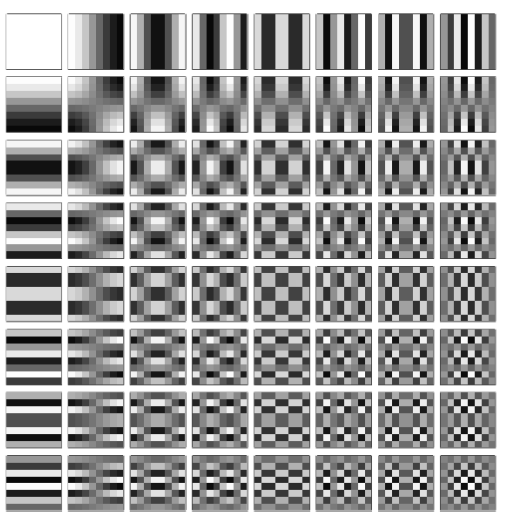
\includegraphics[scale=0.5]{assets/dct_2d.png}\\
  The 64 basis images for the $8{\times}8$ 2D DCT.
  Each is a cosine pattern along both axes.
\end{center}

Used in \textbf{JPEG} compression (lossy).

% ----------------------------------------------------------------
\subsection{Gaussian Pyramids}
\textbf{Goal:} Represent an image at multiple resolution levels, halving each
dimension at every level. The resulting stack of images resembles a pyramid
(coarse at the top, fine at the bottom).

\textbf{Uses:} Multi-scale image analysis, coarse-to-fine optimization, feature
detection at multiple scales (e.g.\ SIFT), and image blending.

\subsubsection{How to Reduce a Signal to Half Its Size}
Naively dropping every other sample causes \textbf{aliasing} (sampling theorem).

\textbf{Fix:}
\begin{enumerate}
  \item \textbf{Smooth} — apply a 1D averaging mask to attenuate high frequencies:
        \[\begin{pmatrix}\tfrac{1}{2} & \tfrac{1}{2}\end{pmatrix}\]
        For $d$ dimensions, apply along each axis independently.
  \item \textbf{Downsample} — keep every second sample.
\end{enumerate}

\paragraph{Example:} Signal $(4,\,2,\,6,\,12)$

After smoothing (with mirroring at the right boundary):
$(3,\,4,\,9,\,12)$

After downsampling (every second value):
$(3,\,9)$

\subsubsection{Formal Definition for 1D}
Signal $u = (u_0,\dots,u_{2^N-1})^T$ with $2^N$ values.

Level $k$ has $2^k$ values ($k \geq 1$), and 1 value at $k = 0$.

The \textbf{restriction operator} $R_k^{k-1}$ (a $2^{k-1} \times 2^k$ matrix)
maps level $k$ to level $k-1$:

\begin{center}
  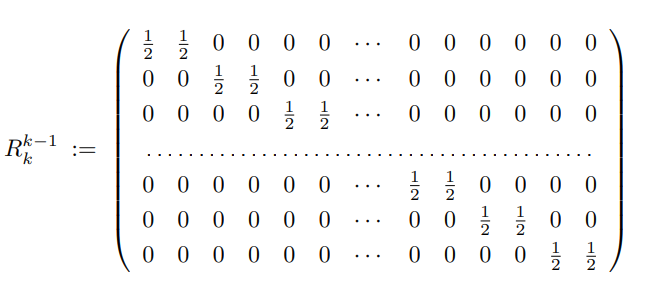
\includegraphics[scale=0.5]{assets/restriction_operator_gaussian_pyramid.png}
\end{center}

The \textbf{Gaussian Pyramid} $\{v^N, \dots, v^0\}$ of $u$:
\[v^N := u\]
\[v^{k-1} := R_k^{k-1} v^k \quad (k = N,\dots,1)\]

\paragraph{Storage cost:}
Although we store many images, total storage stays bounded via the geometric series:
\[
  \sum_{k=0}^{\infty} q^k = \frac{1}{1-q} \quad |q| < 1
\]
\begin{itemize}
  \item 1D: $\approx 2\times$ the original signal size
  \item 2D: $\approx \tfrac{4}{3}\times$ the original image size
\end{itemize}
Pyramid decomposition has \textbf{linear} complexity in both space and time.

\textbf{Limitation:} Not translation-invariant — shifting the signal changes which
samples are picked during downsampling, producing a different pyramid.

\subsubsection{Coarse-to-Fine Strategies}
Running an expensive algorithm on the full-resolution image is slow. Instead:
\begin{enumerate}
  \item Solve the problem on the \textbf{coarsest} (smallest) level.
  \item Use that solution as the starting point for the next finer level.
  \item Repeat up to full resolution.
\end{enumerate}

\paragraph{Example — Gradient Descent:}
On the fine-resolution signal, gradient descent can get trapped in local minima.
The coarser (smoothed) signal washes out many of these traps, making it easier
to find a good global solution. The coarse result then initializes the
fine-grained descent, saving many iterations.

% ----------------------------------------------------------------
\subsection{Laplacian Pyramids}
\label{subsec:laplacian-pyramid}
\textbf{Goal:} Decompose an image into \textbf{frequency bands} — each level
captures the detail lost between two consecutive levels of the Gaussian Pyramid.

\paragraph{Bandpass intuition:}
\begin{itemize}
  \item A \textbf{lowpass filter} keeps only low frequencies (smooth structure).
        Each Gaussian Pyramid level is a lowpass-filtered version of the one above.
  \item Subtracting two consecutive Gaussian levels removes the shared low
        frequencies and keeps only the \textbf{band} of frequencies in between.
        This is a \textbf{bandpass filter}.
  \item Visually: each Laplacian level looks like an edge map — it shows only the
        detail at a particular scale, with large smooth regions zeroed out.
\end{itemize}

\textbf{Construction:}
\begin{itemize}
  \item Upsample (pixel doubling) the coarser Gaussian level to match the finer
        level's resolution.
  \item Subtract: $L^k := v^k - \mathrm{Upsample}(v^{k-1})$
  \item The result is the \textbf{Laplacian Pyramid} $\{L^N, \dots, L^1, v^0\}$.
\end{itemize}
\textbf{Important:} By convention, the last entry of the Laplacian Pyramid is the
coarsest Gaussian level $v^0$ (not a difference), so the original image can be
perfectly reconstructed by summing upward through the pyramid.

\textbf{Note: } When downsampling, and upsample, the average gray value is preserved. This means that in the laplacian pyramid the average gray value is always zero (except at the top, where the value is the average gray value (see convention above)).

\subsubsection{Formal description in 1D}

You are given signal $u=(u_0,\dots,u_{2^N-1})^T$ with Gaussian Pyramid $\{v^N,\dots,v^0\}$

We define the interpolation operator
\begin{center}
  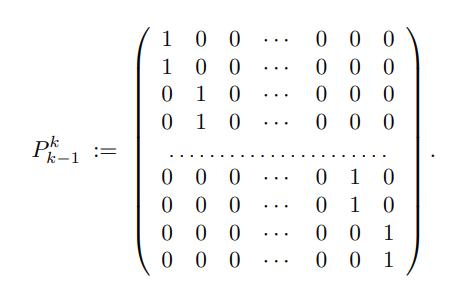
\includegraphics[scale=0.5]{assets/interpolation_operator.png}
\end{center}
And we define the laplacian Pyramid $\{w^N,...,v^0\}$ of u as:
\[w^k := v_k - P^k_{k-1}v^{k-1} \quad (k=N,...,1)\]
\[w^0 := v^0\]


\subsubsection{Applications of Laplacian Pyramids}
Used to assess cloudiness of nonwoven fabric

\subsection{Discrete Wavelet Transform}
We basically want a more compact representation with localisation both in space and frequency.

\subsubsection{Example: Signal representation in different Basis}
We can represent signal $f = (6,4,5,1)^T$ in the following orthonormal basis.
\begin{itemize}
  \item $b_1 := \frac{1}{2}(1,1,1,1)^T$
  \item $b_2 := \frac{1}{2}(1,1,-1,-1)^T$
  \item $b_3 := \frac{1}{\sqrt{2}}(1,-1,0,0)^T$
  \item $b_4 := \frac{1}{\sqrt{2}}(0,0,1,-1)^T$
\end{itemize}
You can imagine the basis as a frequency wave

In the representation $f = \sum_{i=1}^{4}\alpha_i b_i$ we can compute the coefficients $\alpha_i$ pretty easily.

\subsubsection{1-D Haar Wavelet}
The general idea is having a wave-like function with mean 0 (the \textbf{mother wavelet}) that is scaled and shifted ($b_2$ in our case).

An additional basis function with non-vanishing mean \textbf{scaling function} (in our case $b_1$)

\subsubsection{Continous Haar Wavelet}
Simplest wavelet. It uses a step function as mother wavelet

\[\Psi(x) := \begin{cases}
  1 \quad 0 \leq x \leq 1/2\\
  -1 \quad 1/2 < x \leq 1\\
  0 \quad else
\end{cases}\]

We can scale and shift the mother wavelet
\[\Psi_{j,k}(x) := \frac{1}{2^{j/2}}\Psi\left(\frac{x}{2^j}-k\right)\]
j handles the 'squeezing' and k the 'shifting'.

$\Psi_{j,k}$ has width $2^j$ and range $\left[-\frac{1}{2^{j/2}},\frac{1}{2^{j/2}}\right]$. It starts at $k2^j$ and ends at $(k+1)2^j$

\begin{center}
  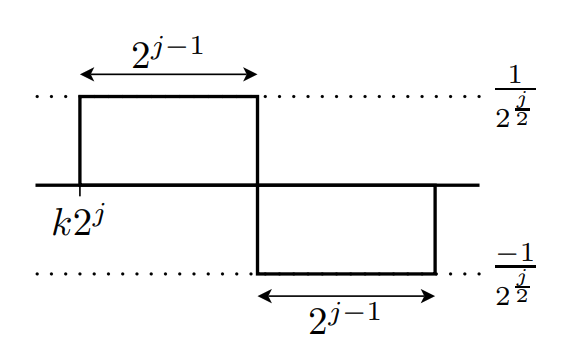
\includegraphics[scale=0.5]{assets/1d_haar_wavelet.png}
\end{center}

\paragraph{Properties}: 
\begin{itemize}
  \item $||\Psi_{j,k}|| = 1$
  \item If $j,k$ are integer numbers, the Haar wavelets $\{\Psi_{j,k}\}$ are orthonormal 
\end{itemize}
For the scaling function we can use a box function $(b_1)$

\[\Phi(x) := \begin{cases}
  1 \quad 0 \leq x \leq 1\\
  0 \quad else
\end{cases}\]
Can also be scaled and shifted
\[\Phi_{j,k}(x) := \frac{1}{2^{j/2}}\Phi\left(\frac{x}{2^j}-k\right)\]
\begin{center}
  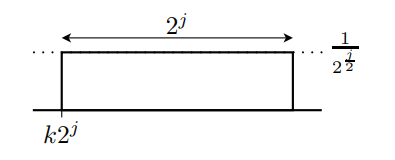
\includegraphics[scale=0.5]{assets/1d_haar_scaling.png}
\end{center}
\subsubsection{Discrete Haar Wavelet}
The previous model was continous to describe scaling and shifting more intuitively. But discrete signals require discrete models

For a discrete signal of length $N = 2^n$ we consider the following functions
\begin{itemize}
  \item $\Phi_{n,0}$ scaling function
  \item $\Psi_{n,0}$ lowest frequency, unlocalized
  \item $\Psi_{n-1,0},\Psi_{n-1,1}$ higher frequency at 2 locations
  \item $\vdots$
  \item $\Psi_{1,0},\Psi_{1,1},\dots,\Psi_{1,2^{n-1}-1}$ Highest frequency at $2^{n-1}$ locations
\end{itemize}
With signal of length $N$, you get $N-1$ wavelet functions and $1$ scaling functions.

To sample, we sample $N$ equidistant points $\{\frac{1}{2},\frac{3}{2},\dots,N-\frac{1}{2}\}$. This creates orthonormal basis of $\mathbb{R}^N$

We identify step functions and scale functions with their vectors $\Phi_{j,k}$ and $\Psi_{j,k}$
\paragraph{Conventions}:
\[c_{j,k} := f^T\Phi_{j,k} \quad \text{ coefficient of the (c for coarse) scaling vector } \Phi_{j,k}\]
\[d_{j,k} := f^T\Psi_{j,k} \quad \text{ coefficient of the (d for detail) wavelet vector } \Psi_{j,k}\]
Coefficients are stored in a coarse-to-fine manner
\[c_{n,0} | d_{n,0} | d_{n-1,0} d_{n-1,1} | \dots | d_{1,0} \dots d_{1,2^{n-1}-1}\]

\subsubsection{Fast Wavelet Transform (FWT)}
With the method before, we have to project the signal of size $N$ to the $N$ basis functions, so the complexity is $O(N^2)$. Maybe there is something better?

The idea is that we have some relation between wavelets we can exploit
\begin{center}
  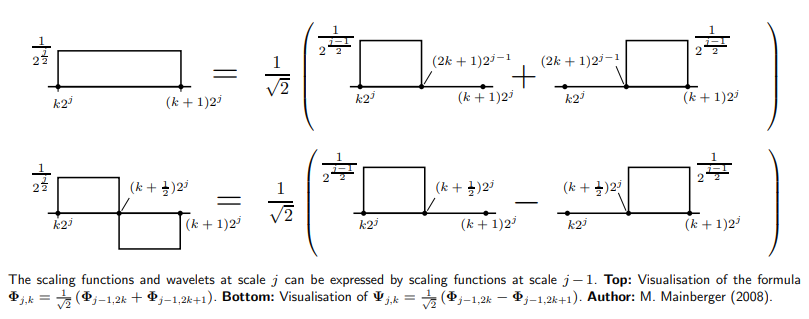
\includegraphics[scale=0.5]{assets/fast_wavelet_transform_idea.png}
\end{center}
We can combine wavelets to get other wavelets basically

\[\Phi_{j,k} = \frac{1}{\sqrt{2}}(\Phi_{j-1,2k} + \Phi_{j-1,2k+1}) \quad (k = 0,...,2^{n-j}-1)\]


\[\Psi_{j,k} = \frac{1}{\sqrt{2}}(\Psi_{j-1,2k} - \Psi_{j-1,2k+1}) \quad (k = 0,...,2^{n-j}-1)\]


Also, at the finest scale $j=0$ (which represents flat functions with a single peak)
\[c_{0,k} = f^T\Phi_{0,k} = f_k \quad (k=0,...,2^n-1)\]

So for scales $j = 1,\dots,n$ we can compute
\[c_{j,k} = \frac{1}{\sqrt{2}}(c_{j-1,2k} + c_{j-1,2k+1})\]
\[d_{j,k} = \frac{1}{\sqrt{2}}(d_{j-1,2k} - d_{j-1,2k+1})\]
starting from the finest scale $j=0$ with the initialisation
\[c_{0,k} = f_k\]

This fine-to-coarse algorithm is called \textbf{Fast Wavelet Transform}. It is $O(N)$
\begin{center}
  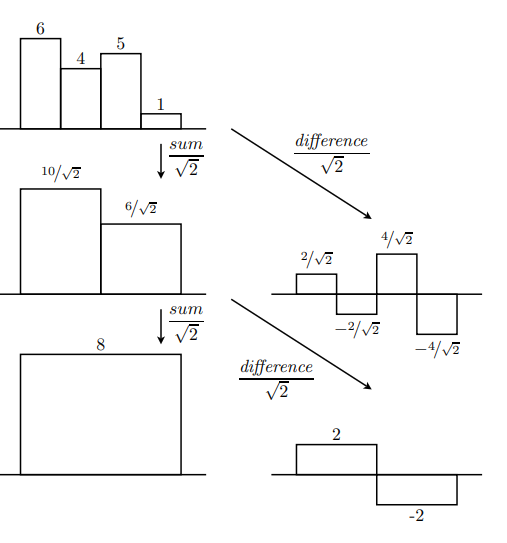
\includegraphics[scale=0.5]{assets/fast_wavelet_transform_result.png}
\end{center}
So in this image our result is the coarse coefficient $c_{2,0} = 8$ and the detailed coefficients $d_{1,0} = \frac{2}{\sqrt{2}}$, $d_{1,1} = \frac{4}{\sqrt{2}}$, $d_{2,0} = 2$
\subsubsection{Inverse Fast Wavelet Transform}
We can just use a similar theorem as above and say
\[\Phi_{j,2k} = \frac{1}{\sqrt{2}}(\Phi_{j+1,k} + \Psi_{j+1,k})\]
\[\Psi_{j,2k} = \frac{1}{\sqrt{2}}(\Phi_{j+1,k} - \Psi_{j+1,k})\]

\begin{center}
  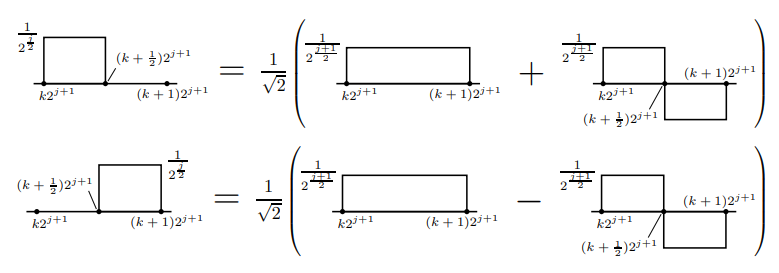
\includegraphics[scale=0.5]{assets/inverse_fast_wavelet_transform.png}
\end{center}
Then we proceed ina  coarse-to-fine manner from $j=n-1$ to $j=0$ and compute

\[c_{j,2k} = \frac{1}{\sqrt{2}}(c_{j+1,k} + d_{j+1,k})\]
\[d_{j,2k} = \frac{1}{\sqrt{2}}(c_{j+1,k} - d_{j+1,k})\]

And the reconstructed signal $f$ is given by $f_k = c_{0,k}$ for $k = 0,\dots,2^n-1$
\begin{center}
  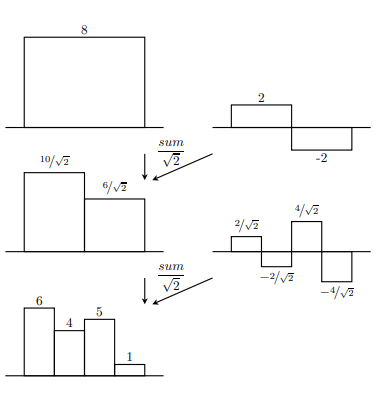
\includegraphics[scale=0.5]{assets/inverse_fast_wavelet_transform_result.png}
\end{center}
\subsection{Wavelets vs Pyramids vs Fourier vs Cosine Representation}
\begin{center}
  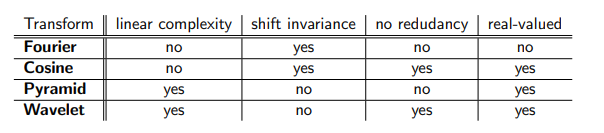
\includegraphics[scale=0.8]{assets/transform_comparison.png}
\end{center}
Lack of redundancy refers to that a signal of length $N$ is represented by $N$ coefficients (this is a good thing)
\subsection{Two Dimensional Wavelet Transform}
There is some sense of separability, so it's not exponentially more complex. You can combine the basis 1-D effects to mix them. You can have box function in one dimension and step function in the other. Mix and match, see below

\begin{center}
  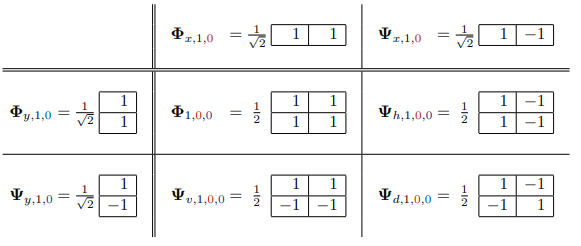
\includegraphics[scale=0.7]{assets/2d_wavelet.png}
\end{center}

Before (in 1D) you had 1 coarse, 1 detail, and now we have 1 coarse, 3 details.

\subsubsection{Fast Wavelet Transform in 2D}
To compute the coefficients in 2D 
\begin{center}
  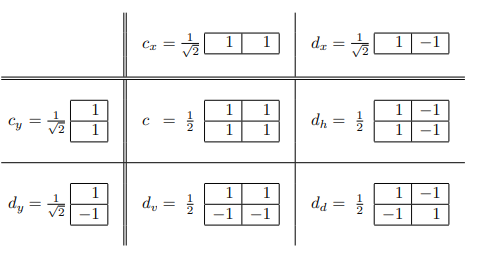
\includegraphics[scale=0.6]{assets/2d_fast_wavelet_transform.png}
\end{center}

\paragraph{Non-standard decomposition}: You start with the wavelet decomposition on a single level, first in x direction and then in y direction. Perform the next decomposition only in the scaling coefficient quadrant. Repeat until single pixel is reached

\begin{center}
  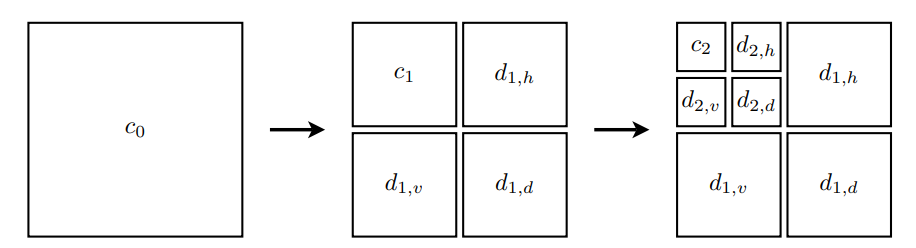
\includegraphics[scale=0.5]{assets/nonstandard_decomposition_wavelet.png}
\end{center}

\section{Image Compression}
Storing raw image data requires vast storage capacity, making efficient compression techniques essential. Compression algorithms are divided into two main paradigms:
\begin{itemize}
  \item \textbf{Lossless Image Compression:} Eliminates structural redundancy without discarding information. It is mathematically exact but less efficient, typically yielding compression rates up to $4:1$.
  \item \textbf{Lossy Image Compression:} Discards psychovisually redundant data that the human eye struggle to perceive. It achieves high efficiency beyond $10:1$ compression rates. The established standard is \textbf{JPEG} (based on the Discrete Cosine Transform), while the modern alternative is \textbf{JPEG2000} (based on the Wavelet Transform).
\end{itemize}

\subsection{Huffman Coding}
Huffman coding is a popular lossless compression technique that optimizes data size by assigning shorter variable-length bit strings to symbols that appear with higher frequency. In digital image processing, these symbols typically map directly to pixel gray values.

This technique is widely deployed in embedded environments like printers, HDTV signal distribution, and network modems.

\paragraph{Algorithmic Concept:} It is governed by a greedy algorithm that builds a prefix-free binary tree bottom-up. Because it satisfies the prefix property (no valid codeword forms the prefix of another), the encoded bitstream requires no explicit delimiters or separator bits between symbols.

\subsubsection{Example: Encoding the word 'ZOOLOGY'}
To compress the 7-letter word \textbf{ZOOLOGY}, we first map out the precise probability distribution of each unique character:
\begin{flalign*}
  & p(Z) = \frac{1}{7}, \quad p(O) = \frac{3}{7}, \quad p(L) = \frac{1}{7}, \quad p(G) = \frac{1}{7}, \quad p(Y) = \frac{1}{7} &
\end{flalign*}

Next, the characters are sorted by ascending probability order to prime the tree builder:
\[
Z, \quad L, \quad G, \quad Y, \quad O
\]
The algorithm repeatedly pairs the two leaf nodes holding the lowest probability weights, merging them into an intermediary parent node whose weight equals their sum.

\begin{center}
  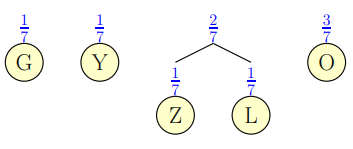
\includegraphics[scale=0.5]{assets/huffman_1.png}
\end{center}
This grouping sequence is executed recursively until a unified, singular root node with a cumulative value of $1.0$ is attained.
\begin{center}
  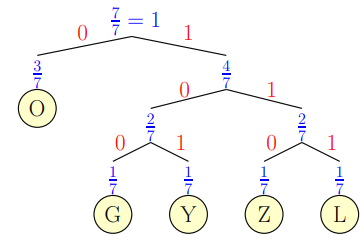
\includegraphics[scale=0.5]{assets/huffman_2.png}
\end{center}
Once the binary tree is structured, we systematically assign a bit value of \texttt{0} to every left branch and a \texttt{1} to every right branch. The final codeword for any symbol corresponds to the path traversed from the root down to its leaf node:

\begin{center}
\begin{tabular}{llc}
  \hline
  \textbf{Symbol} & \textbf{Path Traversal} & \textbf{Resulting Codeword} \\ \hline
  $Z$ & Right $\to$ Right $\to$ Left   & \texttt{110} \\
  $O$ & Left                          & \texttt{0}   \\
  $L$ & Right $\to$ Right $\to$ Right  & \texttt{111} \\
  $G$ & Right $\to$ Left $\to$ Left    & \texttt{100} \\
  $Y$ & Right $\to$ Left $\to$ Right   & \texttt{101} \\ \hline
\end{tabular}
\end{center}

Applying these codes, the word \textbf{ZOOLOGY} condenses into the unified bit sequence:
\[
\text{Code}(\text{ZOOLOGY}) = [\texttt{110}, \texttt{0}, \texttt{0}, \texttt{111}, \texttt{0}, \texttt{100}, \texttt{101}]
\]
This custom variable-length mapping consumes a total of $15\text{ bits}$. Conversely, a uniform fixed-length layout would require $3\text{ bits}$ per symbol to differentiate the 5 unique characters, totaling $3 \times 7 = 21\text{ bits}$. 

By switching to Huffman coding, we successfully shave off approximately $40\%$ of the structural footprint with absolute mathematical fidelity.

\subsubsection{Decoding}
Decoding a Huffman bitstream requires access to the identical dictionary tree topology. The decoder reads incoming bits sequentially, stepping down the branches (\texttt{0} for left, \texttt{1} for right) until it contacts a terminating leaf node. The corresponding symbol is emitted, and the pointer resets instantly to the tree root to parse the subsequent bit.

\subsubsection{Information-Theoretic Considerations}
In information theory, Shannon proves that the mathematically optimal length to encode an independent symbol $k$ appearing with a probability $p_k$ is exactly defined by its self-information:
\[
L_k = -\log_2(p_k) \quad (\text{Note: Let } \operatorname{ld}(x) := \log_2(x))
\]
In our scenario, character $O$ yields an optimal length of $-\log_2(3/7) \approx 1.22\text{ bits}$, while $Z$ requires $-\log_2(1/7) \approx 2.81\text{ bits}$. Because real-world computer architectures require integer bit strings, Huffman codes round these fractional values into practical allocations of $1\text{ bit}$ and $3\text{ bits}$ respectively.

The theoretical baseline for the minimum average bit-depth across the entire source message is defined by the weighted entropy formula $H$:
\[
H = -\sum_{k} p_k \log_2(p_k)
\]
For our text example, this yields an entropy bound of $H \approx 2.13\text{ bits/symbol}$. Our computed Huffman scheme averages $15\text{ bits} / 7\text{ symbols} \approx 2.14\text{ bits/symbol}$, matching the theoretical entropy threshold closely.

\begin{itemize}
  \item Compression algorithms that adapt their bit allocations to scale proportionally with the negative logarithm of symbol probability are formally called \textbf{entropy coding} methods.
  \item Huffman coding stands as the mathematically optimal symbol-by-symbol encoder restricted to integer bit lengths, assuming symbol events are statistically independent and the source probability distribution is known a priori.
  \item \textbf{Note on Arithmetic Coding:} We can approach the absolute non-integer entropy minimum even closer by transitioning to \textbf{Arithmetic Coding}. Instead of mapping symbols to discrete codes, it maps an entire sequence onto a single fluid real-number interval within $[0,1)$. However, commercial usage has historically been constrained by active corporate patents.
\end{itemize}

\subsection{Run Length Encoding (RLE)}
Run-Length Encoding (RLE) is an alternative lossless compression approach that exploits recurring spatial patterns within a sequential signal stream (e.g., compressing an asset string like \texttt{00000000} down into a compact notation like $8 \cdot 0$).

\subsubsection{Modification for Grayscale Images}
Continuous grayscale imagery presents high-frequency fluctuations that destroy traditional RLE performance, as minor deviations prevent long runs of identical pixel values.

\paragraph{Solution: Bitplane Coding}
Because every standard pixel is represented by $8\text{ bits}$, an image can be decomposed into $8$ discrete binary \textbf{bitplanes}. RLE is then executed independently across each spatial bitplane layer. The higher-order, most significant bits (MSBs) contain stable architectural shapes that change infrequently, allowing RLE to compress them with immense efficiency.

An inherent issue with standard binary serialization is that an incremental intensity shift of a single gray value can invert multiple bits simultaneously:
\[
3 = (011)_2 \longrightarrow 4 = (100)_2
\]
This phenomenon disrupts smooth spatial runs across the lower-order bitplanes.

\paragraph{Solution: Gray Code}
To resolve this, data is passed through a \textbf{Gray Code} transformation prior to splitting. Gray codes ensure that adjacent numerical values differ by exactly one single bit flip across the entire sequence.

\begin{center}
  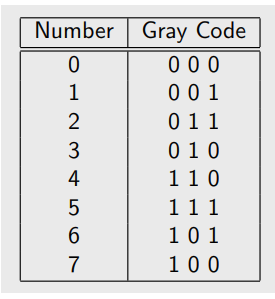
\includegraphics[scale=0.5]{assets/gray_code.png}
\end{center}

\subsection{The JPEG Image Compression Standard}
The \textbf{JPEG} (\textbf{J}oint \textbf{P}hotographic \textbf{E}xperts \textbf{G}roup) standard defines multiple operation layers, including a lossless framework. The most prevalent implementation is the lossy compression pipeline based on the Discrete Cosine Transform (DCT).

The encoder processes a digital image using six sequential steps:
\begin{enumerate}
  \item Convert source graphics from the RGB space into the decoupled \hyperref[sec:YCbCr]{YCbCr} space.
  \item Spatial subsampling of the chroma channels ($Cb, Cr$) to exploit human visual limits.
  \item Partition the channels into $8\times8$ pixel blocks and apply the 2D DCT.
  \item Quantize the resulting continuous coefficients to remove unneeded precision.
  \item Reorder the quantized DCT entries via a frequency-maximizing zigzag scan.
  \item Apply entropy coding to wrap the final values into a packed stream.
\end{enumerate}
The decoding apparatus reconstructs the visible image by executing these steps in exact reverse order.

\subsubsection{Step 1: RGB to YCbCr Transformation}
This initial coordinate transformation serves to isolate raw luminance information ($Y$) from chromatic components ($Cb, Cr$), preparing the channels for independent compression strategies.

\subsubsection{Step 2: Subsampling Chroma Channels}
The physiological structure of the human eye exhibits significantly lower spatial resolution tracking chroma variations ($Cb, Cr$) compared to luminance intensity ($Y$). Taking advantage of this, we downsample both chroma channels by a spatial factor of 2 without introducing visible distortion.

\subsubsection{Step 3: DCT on 8x8 Pixel Blocks}
The 2D Discrete Cosine Transform translates localized spatial pixel configurations into a collection of frequency coefficients:
\begin{itemize}
  \item To optimize the dynamic range requirements of the primary DC coefficient, incoming pixel intervals are level-shifted from unsigned $[0, 255]$ to a zero-centered signed balance of $[-128, 127]$.
  \item The image canvas is partitioned into isolated $8\times8$ blocks under the assumption that localized neighborhoods maintain high spatial consistency.
  \item The 64 output DCT coefficients represent distinct spatial frequencies present inside that block. While this mathematical translation itself is completely lossless, it sets up the data to be compressed easily.
\end{itemize}

\subsubsection{Step 4: Quantization of DCT Coefficients}
Quantization is the primary lossy stage where data size reduction takes place. 

The user controls the targeted compression aggressiveness by scaling a standardized, pre-computed $8\times8$ quantization matrix. Every calculated frequency coefficient within a block is divided by its corresponding matrix value and rounded straight to the nearest integer:
\[
C_{\text{quantized}} = \operatorname{round}\left( \frac{\text{DCT}_{i,j}}{\text{Quantization}_{i,j}} \right)
\]
This intentional precision loss forces smaller, high-frequency coefficients down to zero while compressing remaining values into smaller integer bounds.

\begin{center}
  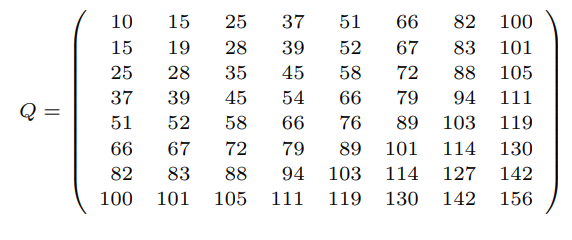
\includegraphics[scale=0.4]{assets/quantisation_matrix.png} \qquad
  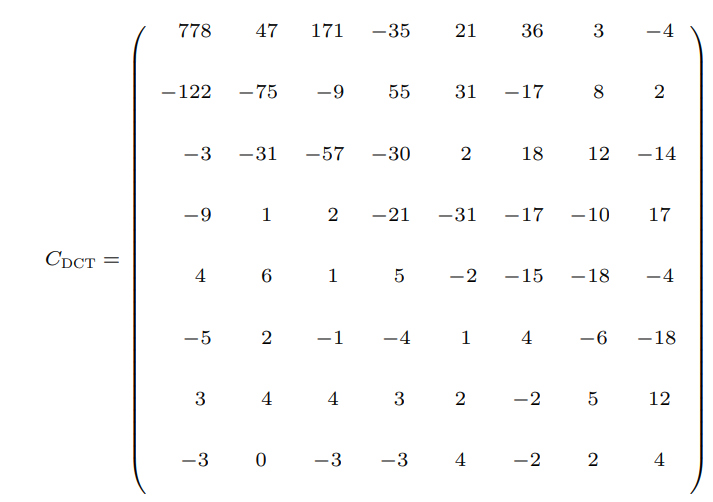
\includegraphics[scale=0.3]{assets/dct_coefficients.png}
\end{center}
\begin{center}
  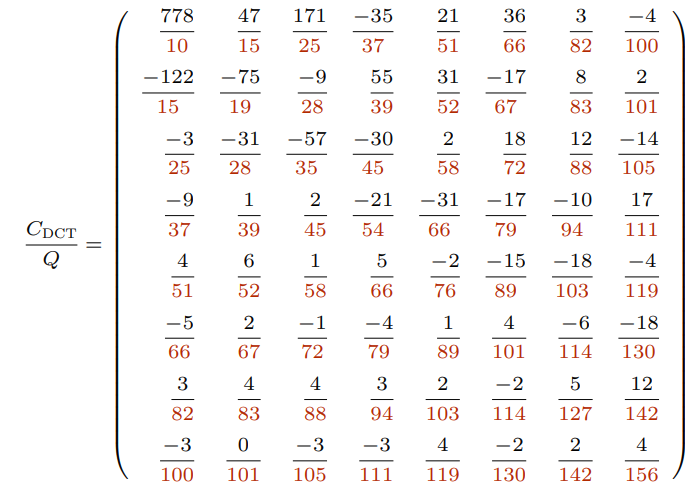
\includegraphics[scale=0.3]{assets/quantisation_matrix_division.png}
\end{center}

\subsubsection{Step 5: Reordering of the DCT Entries}
The quantized 2D matrix is serialized into a 1D stream using a continuous **zigzag scan** pattern that moves from low frequencies to high frequencies. This sweeps the high-frequency coefficients that were rounded to zero into a long, continuous sequence at the tail end of the stream.

\paragraph{Differential DC Coding:} The first entry of each block (the DC coefficient representing average block brightness) is highly correlated with neighboring regions. It is stored as a statistical delta value relative to the DC coefficient of the preceding block, reducing its variance.

\subsubsection{Step 6: Entropy Coding}
The sequenced coefficients are finalized using a customized, two-dimensional variant of Run-Length Encoding. 

Each non-zero coefficient is formatted as a paired metadata descriptor: 
\begin{center}
  \texttt{(Number of preceding zeros, Size class)(Actual coefficient value)}
\end{center}
The size class defines the minimal number of bits required to store the coefficient amplitude, adapting cleanly for negative numbers.

\begin{quote}
\textbf{Example Parameter Walkthrough:} Consider an extracted frequency series following a zigzag read-out: 
\[
[3, -8, 0, -4, 7, -1, 0, 0, \dots, 0]
\]
This sequence is encoded as:
\[
(0,2)(3); \quad (0,4)(-8); \quad (1,3)(-4); \quad (0,3)(7); \quad (0,1)(-1); \quad (0,0)
\]
Where the critical termination marker \texttt{(0,0)} denotes the **End-of-Block (EOB)**. This allows the algorithm to safely drop the long trailing tail of zero entries without wasting any bits.
\end{quote}

\subsection{JPEG 2000}
Developed as the intended successor to the original JPEG standard, JPEG 2000 shifts its mathematical foundation away from localized block-based DCTs to global Discrete Wavelet Transforms (DWT). It eliminates blocky artifacts at high compression configurations and supports multi-resolution scaling, though it remains less prevalent in mainstream consumer applications due to historical computational overhead.

\subsection{Video Compression: MPEG-2}
The idea is that there is (usually) a strong temporal correlation in videos. So an idea is 'predicting' the next frame, and just store the difference between prediction and truth. However, only using the previous frame for prediction doesn't work too well because of motion.

\subsubsection{Motion Compensation}
This is why most codecs use a motion compensation step in the prediction

The image is divided into rectangular blocks, for each block, an equally sized and similar looking block in some \textbf{reference image} is used as prediction. The details depend on the specific codec

\subsubsection{Frame Types}
MPEG-2 uses three different strategies to store frames
\begin{itemize}
  \item Intra-frame (\textbf{I-frame}): No prediction, basically JPEG images
  \item Predicted-frame (\textbf{P-frame}): Codes the difference, prediction is made from the last I- or P-frame
  
  Both I- and P- frames are called \textbf{anchor frames}
  \item Bidirectional frame(\textbf{B-frame}): Codes the difference, predictions are made from the last and next anchor frame. So it's a forward and backward prediction.
\end{itemize}

\subsubsection{GOPs}
Several frames are combined into \textbf{group of pictures (GOPs)}

The first image is usually an I-frame. This allows watching a video at any GOP

\subsubsection{Bitstream order}
Due to different frame types, frames are not always stored in the same order. Example below

\begin{center}
  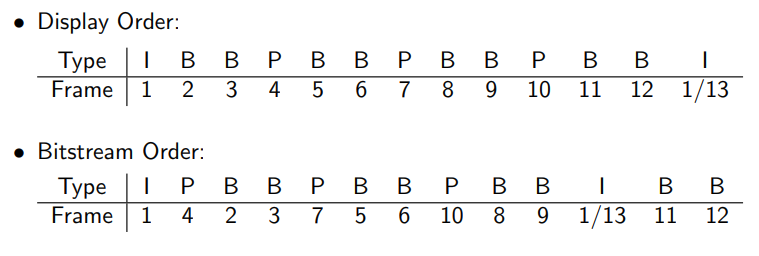
\includegraphics[scale=0.5]{assets/bitstream_order.png}
\end{center}

\section{Point Operations}
\subsection{Definition}
They are image processing operations that convert an image into another, for humans or computers to use better.

The simplest transformations are \textbf{global grayscale modification}. This means that it does not take into account the position of the pixel when changing the value. The only thing that matters is the value

\[\phi: f(x,y) \to g(x,y) = \phi(f(x,y))\]
As you can see, no coordinates are passed onto $\phi$, so it doesn't affect the function. Only the color is passed through

\subsection{Affine Grayscale Transformations}
They have a simple structure
\[g(x,y) = a\cdot f(x,y)  +b\]

For $b = 0$ they are \textbf{linear grayscale transformations}

They allow multiple possibilities
\begin{enumerate}
  \item Identity: $a=1\quad b =0$
  \item Contrast enhancement: $a\geq 1$
  \item Brightening: $a = 1 \quad b > 0$
  \item Grayscale reversion: $a=-1 \quad b = g_{\max}$
\end{enumerate}
The most frequently used is a grayscale transformation to the interval $[0,255]$
\begin{center}
  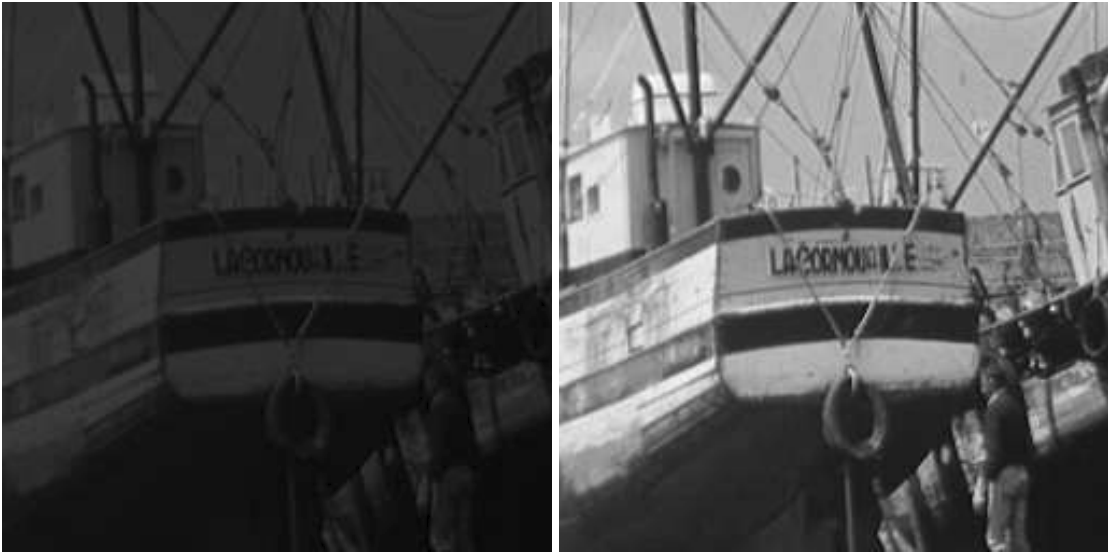
\includegraphics[scale=0.5]{assets/affine_grayscale_transformation.png}
  For an underexposed/overexposed image, we can remap the grayscales to the full gradient, which gives us a more balanced version
\end{center}

\subsection{Non-linear Grayscale Transformations}
\subsubsection{Thresholding}
Can be described as 
\[\phi(f(x,y)): \begin{cases}
  g_{\max} \quad f(x,y) \geq T \\
  0 \quad else
\end{cases}\]
Useful to segment components in an image, like finding a tumor in a brain scan. The hard part is to find parameter $T$

\subsubsection{Logarithmic Dynamic Compression}
For $f(x,y) \geq 0$ one can compute the transformation
\[\phi(f(x,y)) := c\log(1+f(x,y))\]
Usually c is defined so that the max is $255$
\[c := \frac{255}{\log\left(1+\max_{x,y}f(x,y)\right)}\]

It is useful if the dynamic range is too large.

Used mainly in fourier coefficients, where the range is huge, and if for example the first coefficient dominates over the rest, it makes it hard to identify anything useful.

\begin{center}
  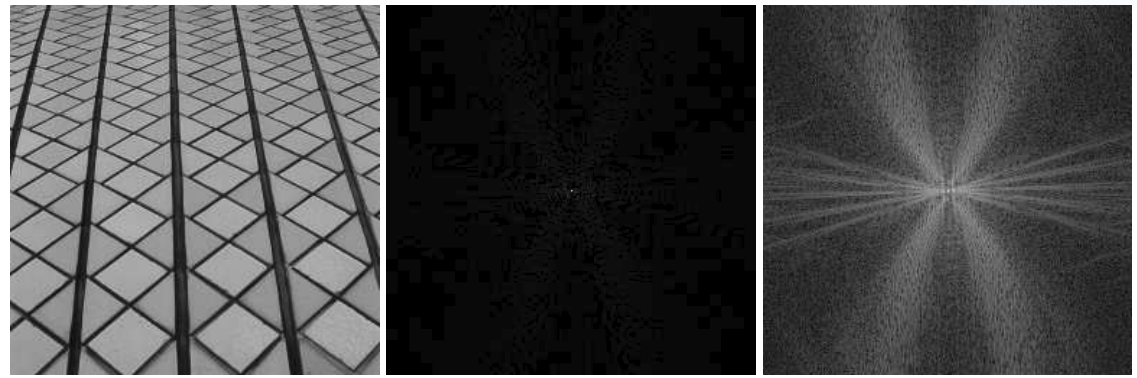
\includegraphics[scale=0.5]{assets/logarithmic_dynamic_compression.png}
  Left image is source, middle is normal fourier coefficients without dynamic logarithmic compression. The middle coefficient dominates so it is hard to see. The right image is after the compression, where the values can be seen better.
\end{center}

\subsubsection{Gamma Correction}
Most video cameras transform light intensity $I$ to a gray value $f$ that is proportional to $I^{\gamma}$, with gamma usualyl being $\approx 0.4$

The value of gamma varies from computer monitor brand. Sometimes even changed by software. This makes it so that some images look ugly on some monitors. So this is why \textbf{gamma correction} is used

For a grayscale image with values in the range $[0,f_{\max}]$ it is given by
\[\phi(f(,x,y)) := f_{\max}\cdot \left(\frac{f(x,y)}{f_{\max}}\right)^{1/\gamma} \quad (\gamma > 0)\]
So the range is not affected, but the correction is applied
\begin{center}
  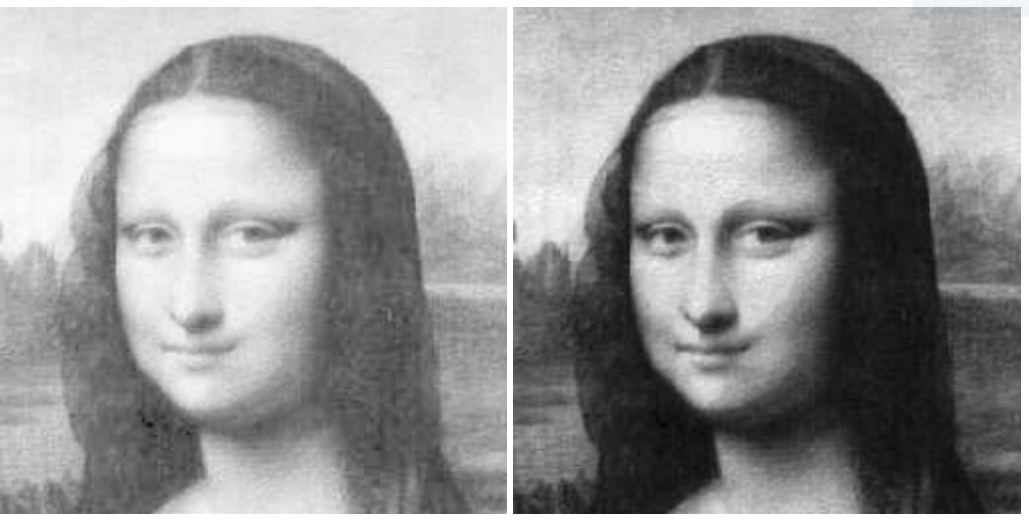
\includegraphics[scale=0.5]{assets/gamma_correction.png}
  Gamma correction with $\gamma = 0.4$
\end{center}

\subsection{Histogram Equalisation}
Function $\phi$ depends on entire gray level set. $\{f(x,y) | (x,y)\in \Omega\}$

The idea is to make it so that all gray values occur equally as often. Usually provokes a dramatic improvement in image quality.s

A \textbf{histogram} specifies how often a gray value appears in an image. Spatial context as usual does not matter.

\paragraph{Algorithm for Direct Histogram Equalisation of a Discrete Image}: The idea is an area-based mapping from one histogram $p_i$ to another hopefully (equalised) histogram $q_i$

Given: 
\begin{itemize}
  \item $p_i$ number of pixels of image $f$ having gray value $v_i \quad (i=1,\dots,m)$
  \item $q_j$ desired number of pixels of $g$ with gray value $w_j \quad (j=1,...,n)$
\end{itemize}
Set $k_0 = 0$
\begin{enumerate}
  \item for r = 1,...,n
  \item Search largest index $k_r \leq m$ with 
  \[\sum_{i=1}^{k_r}p_i \leq \sum_{j=1}^{r}q_j\]
  and map the gray values \[v_{k_{r-1}+1},...,v_k \text{ to } w_r\]
\end{enumerate}

\paragraph{Example}: Imagine an image with $N=16$ pixels and $2^2 = 4$ different gray values. So the $q_i = \frac{16}{4} = 4$ is the desired number of pixels with each value.

\begin{center}
  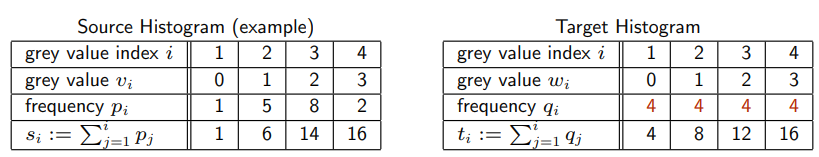
\includegraphics[scale=0.5]{assets/histogram_equalization_example_1.png}
\end{center}

So according to the algorithm, we are looking for the largest index $k_r$ ($r = 1,...,4$) such that $s_{k_r} \leq t_r$
\begin{center}
  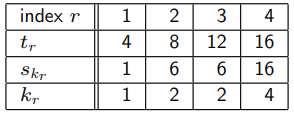
\includegraphics[scale=0.5]{assets/histogram_equalization_example_2.png}
\end{center}

So now we just do the mapping

\begin{center}
  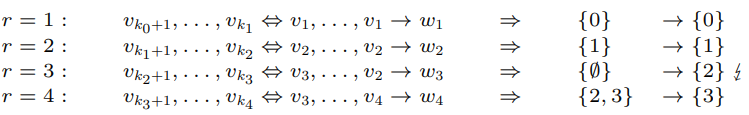
\includegraphics[scale=0.5]{assets/histogram_equalization_example_3.png}
\end{center}

\paragraph{Remarks}: This algorithm can also do \textbf{histogram specification}. And for a general discrete image, this equalisation can only be approximated

\subsection{Pseudocolor representation of grayscale images}
Humans can only distinguish around 40 grayscales and 2000000 colors. So coloring gray values improves distinction.

So the idea is to get a mapping
\[f(x,y) \to \begin{pmatrix}
  \phi_r(f(x,y)) \\
  \phi_g(f(x,y)) \\
  \phi_b(f(x,y))
\end{pmatrix}\]
Used in e.g X-ray scanners in airports

\subsection{False Color Representation of Vectorial Images}

Transforms a multichannel image into a color image. Used in satellite imaging mainly.

\begin{center}
  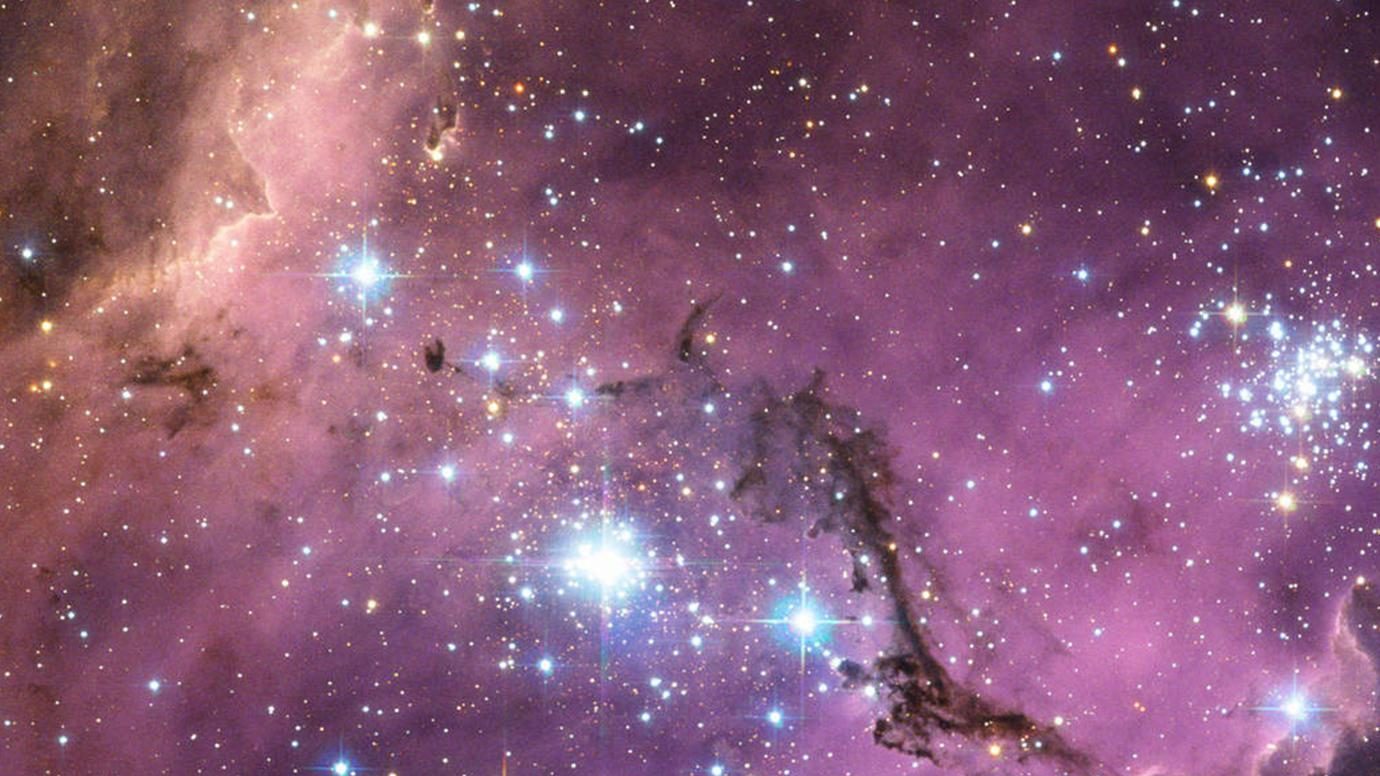
\includegraphics[scale=0.3]{assets/galaxy_multichannel.jpg}
\end{center}
\subsection{Adding Images}
Some imaging methods create a ton of noise

\[\underbrace{g(x,y)}_{\text{noisy}} = \underbrace{f(x,y)}_{\text{no noise}} + \underbrace{n(x,y)}_{\text{noise}}\]

So the idea is that if we can take images of the same object multiple times, we can average out the images to reduce noise.

For uncorrelated noise with mean 0, averaging M images with noise variance
\[\sigma^2= \frac{1}{|\Omega|}\int_{\Omega}|n(x,y)|^2dxdy\]
creates a reduced noise variance $\overline{\sigma}^2 = \sigma^2/M$ which results in a reduced standard deviation $\overline{\sigma} = \sigma/\sqrt{M}$

\begin{center}
  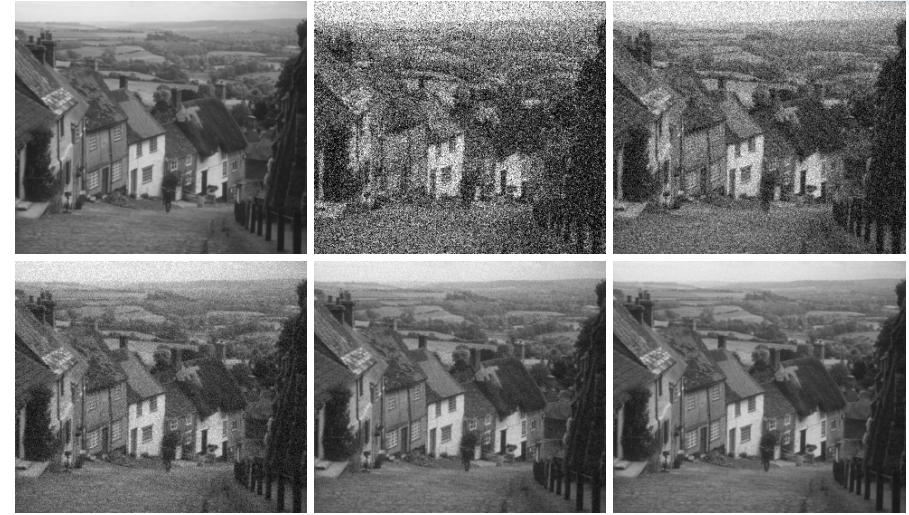
\includegraphics[scale=0.5]{assets/noise_averaging.png}

Images: from left to right, top to bottom
\begin{enumerate}
  \item Original image, $\sigma = 52.29$
  \item Gaussian noise with standard deviation $52.29$ added
  \item Averaged 4 times
  \item Averaged 16 times
  \item Averaged 64 times
  \item Averaged 256 times
\end{enumerate}
\end{center}
\subsection{Subtracting Images}
Mainly used with DSA (Digital Subtraction Angiography). It's a medical imaging strategy to visualize blood flow through vessels.

The idea is taking X-rays images before and after giving a flourescent contrast agent. The difference makes active vessels visible.
\begin{center}
  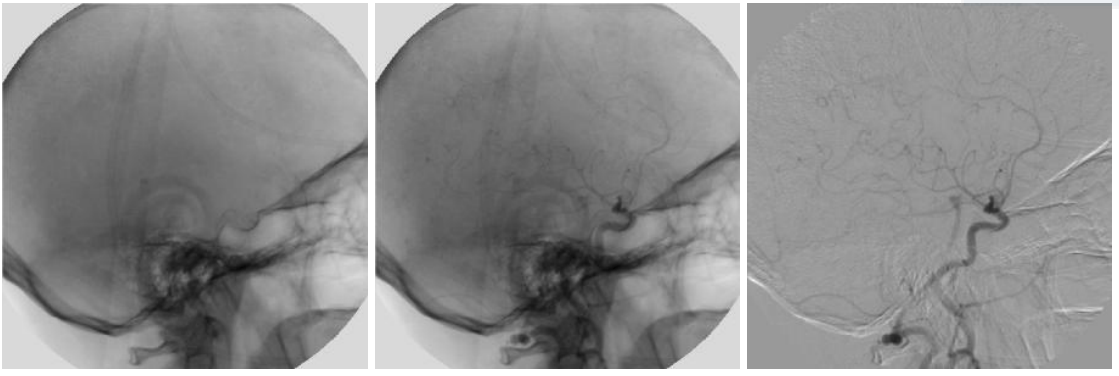
\includegraphics[scale=0.5]{assets/dsa_vessels.png}
  Left is initial image, middle is after giving contrast agent. Right is difference
\end{center}

\section{Linear Filters}
Compute value of pixel in base of linear combination of it's neighbors

\subsection{Linear System Theory}
A \textbf{linear system} L satisfies the \textbf{Superposition principle}
\[L(\alpha f_1 + \beta f_2 ) = \alpha Lf_1 \beta Lf_2\]
for all images $f_1$ and $f_2$ and numbers $\alpha$ and $\beta$

And specifically, the \textbf{Linear Shift Invariant (LSI) System: } The result of the filter depends only on the input singal, but not on the localisation of the signal structure

\[LT_bf = T_bLf\]
For all translations $T_b$ with $(T_b)f(x) = f(x-b)$

\subsubsection{Impulse Response of a Discrete LSI System}
The impulse response of a discrete LSI filter L is the result of filtering a \textbf{Dirac delta impulse}: 
\[h = L\delta_0\]

where $\delta_0 = (\delta_{0,i})$ with the \textbf{Kronecker symbol}

\[\delta_{i,j} = \begin{cases}
  1 \quad i = j \\
  0 \quad else
\end{cases}\]
So $\delta_0$ is like a sequence of peaks of some sort

So because every signal $f = (f_1,...,f_N)^T$ can be represented as a linear combination of N unit impulses $\delta_1,...,\delta_N$. 
\[Lf = L\sum_{i=1}^Nf_i\delta_i = L\sum_{i=1}^N f_i(T_i\delta_0) = \sum_{i=1}^Nf_iLT_i\delta_0 = \sum_{i=1}^Nf_iT_iL\delta_0 = \sum_{i=1}^Nf_iT_ih \]
Remember that $T_i$ is the shift operator. So this show, if we know the response to a single spike, so $T_i\delta_0$ is the same spike but 'delayed'.

This shows that any LSI system is completely characterised by its impulse response. This closely relates to convolution.

\paragraph{Properties of convolution: }
\begin{itemize}
  \item Linearity
  \item Shift invariance 
  \[T_b(f\ast w) = (T_bf)\ast w\]
  \item Commutativity
  \item Associativity
\end{itemize}
And most importantly the \textbf{convolution theorem of the fourier transform}
\[\mathcal{F}[f\ast w] = \mathcal{F}[f]\cdot \mathcal{F}[w]\]
\subsubsection{Basic Types of LSI Filters}
\begin{itemize}
  \item Lowpass filters: Low frequencies are \textbf{less} attenuated than higher ones
  \item Highpass filters: High frequencies are \textbf{less} attenuated than lower ones.
  \item Bandpass filters: Structures within a specific frequency band are barely attenuated.
\end{itemize}

\subsubsection{Lowpass filter}
The idea is to smooth an image by eliminating noise and small-scale details.

Two ways to do it
\paragraph{Lowpass filter in the spatial domain}: Box Filters

Basically, it uses a convolution mask of size $(2m+1) \times (2m+1)$ with weights $\frac{1}{(2m+1)^2}$. Intuitively, a 2D box with all the same values.

Arguments against/in favor
\begin{itemize}
  \item It is separable, so each direction can be applied independently
  \item Total complexity is linear and independent of mask size. (1 addition, subtraction and multiplication per pixel in 1D)
  \item Not rotationally invariant (prefers vertical/horizontal) over for example diagonal
  \item The continous FT of a box function is the $sinc = \sin(x)/x$ function
  \item Not satisfactory in the frequency domain, still oscillates and maybe attenuates too weakly.
\end{itemize}

\paragraph{Lowpass filter in the Frequency Domain}: The Ideal lowpass

All frequency components $(u,v)$ with $u^2+v^2 > T^2$ are set to 0. Still pretty bad, ringing artifacts appear, sinc-like rotation invariant function.

\paragraph{Lowpass filter with a compromise}: Gaussian convolution Kernel

The good thing about this is that the FT of a gaussian is still a gaussian and rotationally invariant. 

Pros about it
\begin{enumerate}
  \item One maximum in both spatial and frequency domain
  \item Only convolution kernel that is both separable and rotationally invariant
  \item Can be implemented efficiently
\end{enumerate}

Formula for $m$-dimensional (isotropic) Gaussian
\[K_\sigma(x) := \frac{1}{(2\pi\sigma^2)^{m/2}}\exp\left(-\frac{|x|^2}{2\sigma^2}\right)\]
\begin{center}
  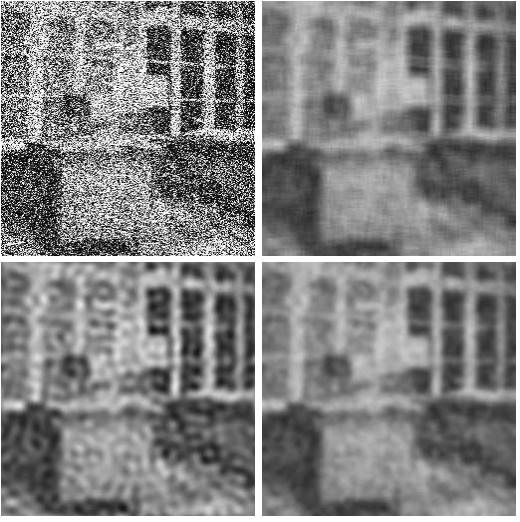
\includegraphics[scale=0.5]{assets/lowpass_filters.png}
  \begin{itemize}
    \item Top left: original
    \item Top right: 11x11 box filter creates vertical and horizontal artifacts
    \item Bottom left: Ideal lowpass $T^2=500$, ringing artifacts
    \item Bottom right: Smoothing with a Gaussian $\sigma=3$
  \end{itemize}
\end{center}

\paragraph{Approximating the Gaussian}: 4 possibilities
\begin{enumerate}
  \item \textbf{Sampling of the Gaussian in the Spatial Domain}: Just splitting and sampling at certain points. Restrict sampling to interval $[-k\sigma, k\sigma]$ (works well for $k\geq 3$)
  
  You have to normalize sum of coefficients to 1

  The good thing is that it is really simple and flexible

  The bad thing about this is the mask size and complexity increases with $\sigma$. Good for small $\sigma$ values

  \item \textbf{Multiplication in the Fourier Domain}: Use FFT to transform the image into the Fourier Domain. Multiply with he FT of the Gaussian, use FFT for the backtransform.
  
  It has $O(N\log N)$ complexity for a square image of N pixels. And complexity doesn't increase with $\sigma$. Good with large $\sigma$ values

  The bad thing is that FFT requires image sizes powers of 2, and wraparound errors.

  \item \textbf{Binomial Kernels}: Use the known binomial kernel
  
  \begin{center}
    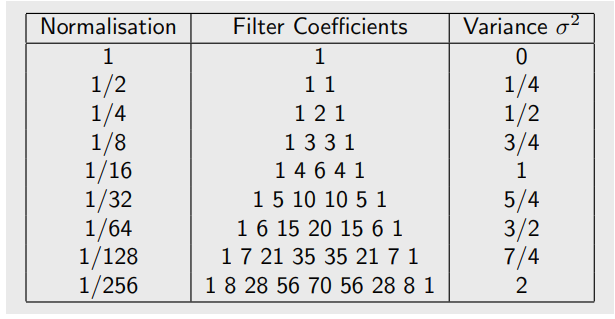
\includegraphics[scale=0.5]{assets/binomial_kernel.png}
    
    These can be shown to approximate gaussians. The Variance column represents the approximate variance they simulate
  \end{center}

  The advantage is that it can be done with integer arithmetic (dividing by 2 is a bit shift).

  The disadvantage is that complexity increases with $\sigma$
  \item \textbf{Iterated Box Filters}: Idea is that box filter is not good, but very efficient. If we use the central limit theorem, we can know that iterated averaging kernels converge to Gaussians. Iterating a box filter three times is usually pretty good.
  
  Can be shown that n iterations of box filter of length l approximate a Gaussian with 
  \[\sigma^2 = n\cdot \frac{l^2-1}{12}\]
  With $l=2$ we get binomial kernels. Good because independence of $\sigma$ and linear complexity, bad because of lack of continuously tuning $\sigma$

\end{enumerate}
\subsubsection{Highpass Filters}
Remove low frequency perturbations. Also sharpens blurry image structures.

\paragraph{Design in the Spatial Domain}: Can be computed as the difference between identity and lowpass. So it's somewhat the additive inverse, because identity does nothing, and lowpass removes low frequencies, so the difference removes high frequencies. 

\begin{center}
  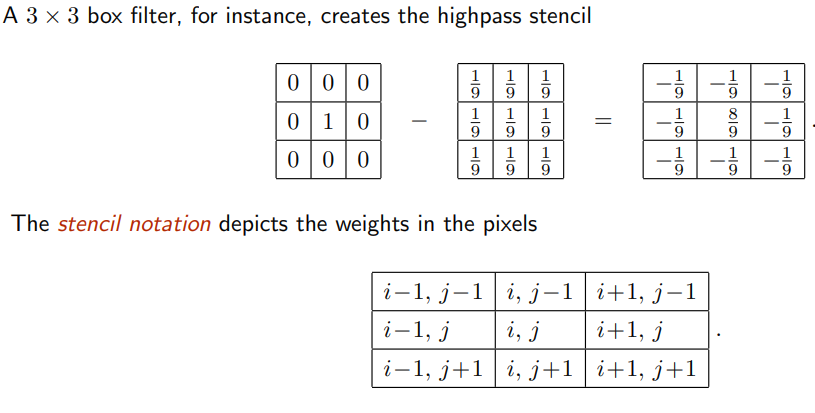
\includegraphics[scale=0.65]{assets/highpass_filter.png}
\end{center}

Displaying the image usually requires an affine rescaling of gray values. This is because for many highpass filters the average gray value becomes zero (if the lowpass preserves the same gray value). Also, negative results are also common

\subsubsection{Bandpass filters}
Not so important for image enhancement, but useful to extract certain image structures at certain scales (e.g cloudiness of fabrics).

Can be created by subtracting two lowpass filters. If the lowpass flters are Gaussians, the bandpass is called \textbf{DoG (Difference of Gaussians)}

\subsection{Edge detection}
\subsubsection{Introduction}
Edges are important because:
\begin{itemize}
  \item They represent strong change of gray values within a neighbourhood
  \item Often provide the most relevant information
  \item They usually represent object boundaries
  \item Give a sparser image representation, rather than definining all pixels
\end{itemize}
Scanning is usually done through \textbf{derivative filters}. The intuition is that a change of gray value means the gray value 'graph', changes. This means that the magnitude of the first derivative is maximal, or where the second terivative has a zero-crossing.

\subsubsection{Problem}
Small, but high frequent fluctuations in the original signals can gravely affect the derivatives.

\paragraph{Example}: Imagine a high frequent 1-D perturbation
\[f(x) = \varepsilon\sin\left(\frac{x}{\varepsilon^2}\right)\]
It becomes arbitrarily small in magnitude for $\varepsilon \to 0$, but it's derivative
\[f'(x) = \frac{1}{\varepsilon}\cos\left(\frac{x}{\varepsilon^2}\right)\]
exceeds all bounds.

\paragraph{Alternative interpretation}: Derivatives in the spatial domain become multiplication in the Fourier domain. So high-frequency components are enormously amplified
\[\mathcal{F}\left[\frac{\partial^{n+m}f}{\partial x^n\partial y^m}\right](u,v) = (i2\pi u)^n(i2\pi v)^m\mathcal{F}[f](u,v)\]
So high frequency components are enormously amplified, because the amplitude of the frequency $u$ and $v$ is proportional to its own frequency in the formula. So for an infinitely big $u$, its amplitude is infinite. 


\paragraph{Remedy}: Lowpass filter before computing derivatives. Usually done with a Gaussian Convolution

\subsubsection{Taylor Expansion}
\paragraph{One Dmensional Taylor Expansion}: A function $f:\mathbb{R}\to\mathbb{R}$ that is (n+1) times continuously differentiable with bounded derivatives can be represented in $x+h$ by it's taylor expansion around x
\[f(x+h) = \sum_{k=0}^n\frac{h^k}{k!}f^{(k)}(x) + O(h^{n+1})\]

\paragraph{Two Dimensional Taylor Expansion}: Same thing just a bit different
\[f(x+h) = \sum_{k=0}^n\frac{1}{k!}\langle h,\Delta\rangle^k f(x) + O(|h|^{n+1})\]
where we have
\[\langle h,\Delta \rangle^2 = (h_1\partial_{x_1} + h_2\partial_{x_2})^2 = h_1^2\partial{x_1x_1} + 2h_1h_2\partial_{x_1x_2} + h^2\partial_{x_2x_2}\]

\subsubsection{Numerical Approximation of Derivatives}
Images/signals are discrete, so direct derivatives are tough. Finite difference approximations of derivatives are obtained by Taylor expansion with comparison of coefficients.

\paragraph{Example}: Get $u_i''$ in pixel i with stencil that takes into account pixels $i-1$;$i$,$i+1$. Grid size is h. We need to compute the stencil weights $h$

\begin{itemize}
  \item $u_{i-1} = u_i - hu_i' + \frac{h^2}{2}u_i'' - \frac{h^3}{6}u_i''' + \frac{h^4}{24}u_i'''' - \frac{h^5}{120}u_i''''' + O(h^6)$   
  \item $u_i = u_i$
  \item $u_{i-1} = u_i + hu_i' + \frac{h^2}{2}u_i'' + \frac{h^3}{6}u_i''' + \frac{h^4}{24}u_i'''' + \frac{h^5}{120}u_i''''' + O(h^6)$
\end{itemize}

We compare the coefficients $\alpha$

\[\alpha_{-1}u_{i-1} + \alpha_0 u_i + \alpha_1u_{i+1}\]
Our goal is given we want the second derivative
\[0u_i + 0u_i' + 1u_i''\]

Substitute with taylor expansion(reduced version)
\[\alpha_{-1}(u_i - hu_i' + \frac{h^2}{2}u_i'' + O(h^3)) + \alpha_0 u_i + \alpha_1(u_i + hu_i' + \frac{h^2}{2}u_i'' + O(h^3))\]
Group by derivative
\[\underbrace{(\alpha_{-1} + \alpha_0 + \alpha_1)}_{=0}u_i + \underbrace{h(-\alpha_{-1}+\alpha_1)}_{=0}u_i' + \underbrace{\frac{h^2}{2}(\alpha_{-1} + \alpha_1)}_{=1}u_i'' + O(\underbrace{(\alpha_{-1}+\alpha_1)}_{\text{may depend on h}}h^3)\]

We want the first two components to be zero and the third to be one to compute the second derivative. This guides us to the following system of equations
\[\begin{pmatrix}
  1 & 1 & 1 \\
  -1 & 0 & 1 \\
  1 & 0 & 1
\end{pmatrix}\begin{pmatrix}
  \alpha_{-1} \\
  \alpha_0 \\
  \alpha_1
\end{pmatrix} = \begin{pmatrix}
  0 \\
  0 \\
  2/h^2
\end{pmatrix}\]
Note that we obtain a 3x3 system because we use three pixels for approximation, and we consider only the first three terms of the Taylor expansion. 

The solution of the linear system gives us 
\[\alpha_{-1} = \frac{1}{h^2} \quad \alpha_0 = \frac{-2}{h^2} \quad \alpha_1 = \frac{1}{h^2}\]
So now, if we convolude the image with this kernel, in theory we should get an approximation of the second derivative at each pixel.

And we can also quantify the approximation error
\[\frac{1}{h^2}u_{i-1} - \frac{2}{h^2}u_i + \frac{1}{h^2}u_{i+1} = \underbrace{0u_i + 0u_i' + 1u_i''}_{\text{per construction}} + \frac{h^3}{6}(\underbrace{-\alpha_{-1} + \alpha_1}_{= 0\text{ ,lucky!}}) + \frac{h^4}{24}(\underbrace{\alpha_{-1} + \alpha_1}_{2/h^2})u_i'''' + O(h^3) = \]
\[= u_i'' + \frac{h^2}{12}u_i'''' + O(h^3) = u_i + O(h^2)\]
The power of the error in the grid size h is called \textbf{consistency order} 2. Note that the 'per construction' part only applies right now, as we set the weights to set the first three terms to our desired values. In general, you also need to compute the error for these terms.

Higher consistency order gives better acccuracy ($h \leq 1$ always, it's the step size). Discretisations must have consistency order at least 1, so that as $h\to 0$ the expression is approximated. Otherwise the method is \textbf{inconsistent}

\subsubsection{Derivative Filters in 1-D}
Most important approximations
\begin{itemize}
  \item First derivative
  \[u'_i = \frac{u_{i+1} - u_i}{h} + O(h) \quad \text{ forward difference}\]

  \[u'_i = \frac{u_i - u_{i-1}}{h} + O(h) \quad \text{ backward difference}\]

  \[u'_i = \frac{u_{i+1} - u_{i-1}}{2h} + O(h^2) \quad \text{ central difference}\]
  \item second derivative
  \[u''_i = \frac{u_{i+1} - 2u_i  + u_{i-1}}{h^2} + O(h^2) \quad \text{ central difference}\]
 
\end{itemize}
Central differences usually have higher order of consistency. The symmetry helps with cancellation effects of some Taylor coefficients.

\paragraph{How to improve Order of Consistency}: By extending stencil size, we can increase order of consistency (and computational effort)
\[u_i' = \frac{u_{i+1} - u_{i-1}}{2h} + O(h^2)\]
\[u_i' = \frac{-u_{i+2} + 8u_{i+1} - 8u_{i-1} + u_{i-2}}{12h} + O(h^4)\]
And so on.

\subsubsection{Derivative Filters in 2-D}
Basically the 1-D masks can also be used in 2-D. So for first order derivatives, the following have consistency order 2

\begin{center}
  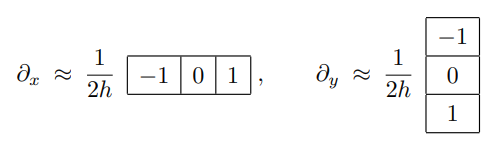
\includegraphics[scale=0.5]{assets/derivative_filter_2d_mask.png}
\end{center}

The issue is that the mask smooths in direction of derivative, but not orthogonal to it. So this suggests to introduce some smoothing perpendicular to the derivative direction.

\paragraph{Sobel Operators}: They convolute with the binomial kernel. This does not deteriorate consistency order.
\begin{center}
  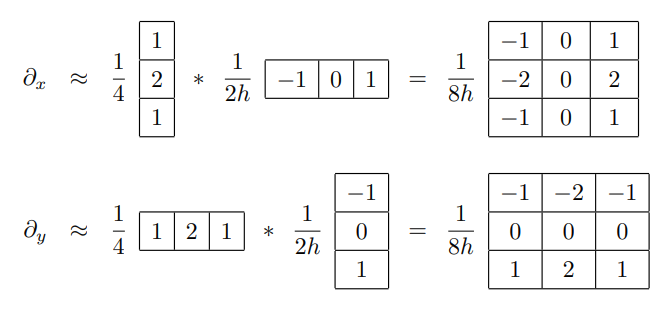
\includegraphics[scale=0.5]{assets/sobel_operators.png}
\end{center}
Also help compute the gradiant magnitude better

\paragraph{Second order derivatives}: Standard approximation of the Laplacian $\Delta u = \partial_{xx}u + \partial_{yy}u$

TODO
\begin{center}
  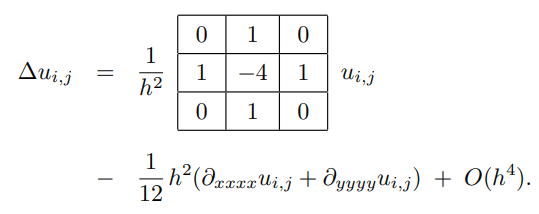
\includegraphics[scale=0.5]{assets/laplactian_second_order_derivative.png}
\end{center}
The issue is that even though Laplacian is rotationally invariant, the derivative expression $\partial_{xxxx}u_{i,j} + \partial_{xxxx}u_{i,j}$ that occurs in the leading error term is not.

Better results can be found with 
\begin{center}
  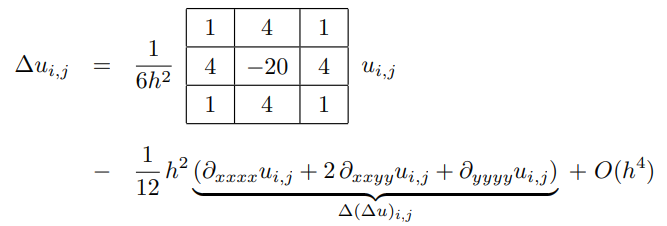
\includegraphics[scale=0.5]{assets/laplactian_second_order_derivative_2.png}
\end{center}

\subsubsection{Edge Detection with First Order Derivatives}
The rough idea is convolve the initial image f with a Gaussian $K_\sigma$ to attenuate high frequencies
\[u = K_\sigma \ast f\]
Compute the gradient magnitude
\[|\nabla|u = \sqrt{(\partial_xu)^2 + (\partial_yu)^2}\]

Extract image regions where $|\nabla u|$ exceeds a certain threshold T

\begin{center}
  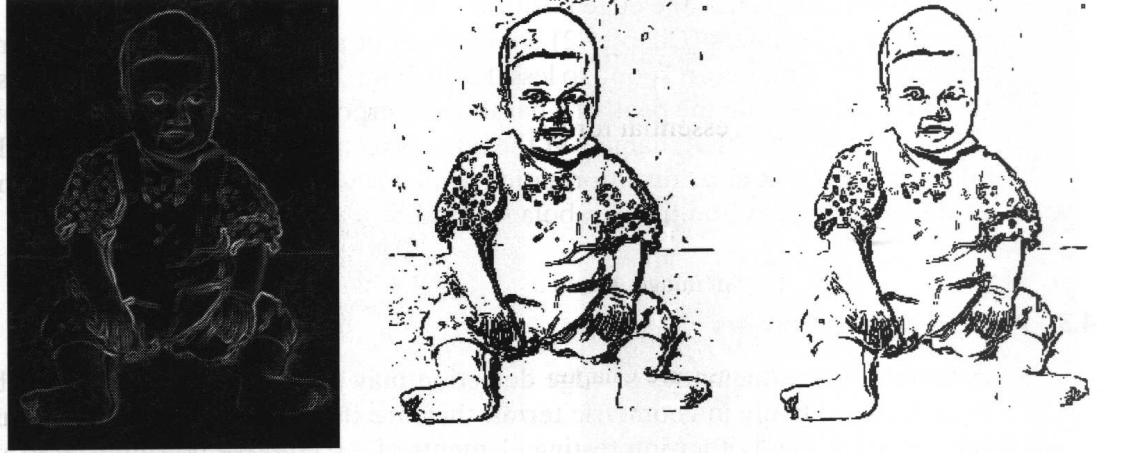
\includegraphics[scale=0.45]{assets/edge_detection.png}
  Left is gradiant magnitude through sobel operators, middle is $T = \sqrt{35}$, too thick edges. Right is $T = \sqrt{50}$, much better but destroys some edges
\end{center}

Advantages
\begin{itemize}
  \item The use of first order derivative is more robust than second order derivatives to avoid noise.
\end{itemize}

Disadvantages
\begin{itemize}
  \item Additional threshold parameter T (beside $\sigma$ of Gaussian)
  \item Some edges are too thick, some below the threshold
  \item Does not create closed contours
\end{itemize}

Remark 
\begin{itemize}
  \item Suitable value for T strongly depends on $\sigma$
  \item Can be convenient to select T as a quantile of the histogram of $|\nabla u|$ So that a certain percentage of the image is kept as edges.
\end{itemize}

\subsubsection{Canny Edge Detector}
Very popular with sophisticated postprocessing. Good performance, with three steps and three parameters
\begin{enumerate}
  \item Gaussian standard deviation $\sigma$
  \item Two thresholds $T_1$,$T_2$
\end{enumerate}

Steps
\begin{enumerate}
  \item Gradiant Approximation by Gaussian Derivatives
  \begin{itemize}
    \item For Gaussian-smoothed image u, compute magnitude $|\nabla u|$, and the orientation angle $\theta = \arg(\nabla u)$ of $\nabla u$
    \item Identify edge candidates as locations where $|\nabla u|$ exceeds low Threshold $T_1$
  \end{itemize}
  \item Nonmaxima suppression: 
  \begin{itemize}
    \item Goal: thinning edges to 1 pixel wide 
    \item In every edge candidate, look at all four directions and select the one that is most 'orthogonal' to edge contour.
    \item If one of the two neighbours in this direcion has a larger gradient magnitude, mark the central pixel.
    \item After passing through all candidates, removed marked pixels from edge map.
  \end{itemize}
  \item Hysteresis Thresholding (Double Thresholding)
  \begin{itemize}
    \item Goal: Extract only relevant edges
    \item Use points above upper threshold $T_2$ as seed points for relevant nedges
    \item Add all neighbours that are above lower threshold $T_1$
  \end{itemize}
\end{enumerate}
\subsubsection{Edge Detection with Second Order Derivatives}
The rough idea is:
\begin{itemize}
  \item Perform Gaussian smoothing on the original image: $u = K_\sigma \ast f$
  \item Compute the Laplacian: $\Delta u := \partial_{xx}u + \partial_{yy}u$ (Laplacian-of-Gaussian (LoG), Marr-Hildreth Operator)
  \item Extract Edges as zero-crossings of the Laplacian (using the intermediate/middle value theorem; if one value is positive and the next is negative, the contour between them is an edge).
\end{itemize}
The stronger the smoothing, the 'weaker' the edge detection.

\begin{center}
  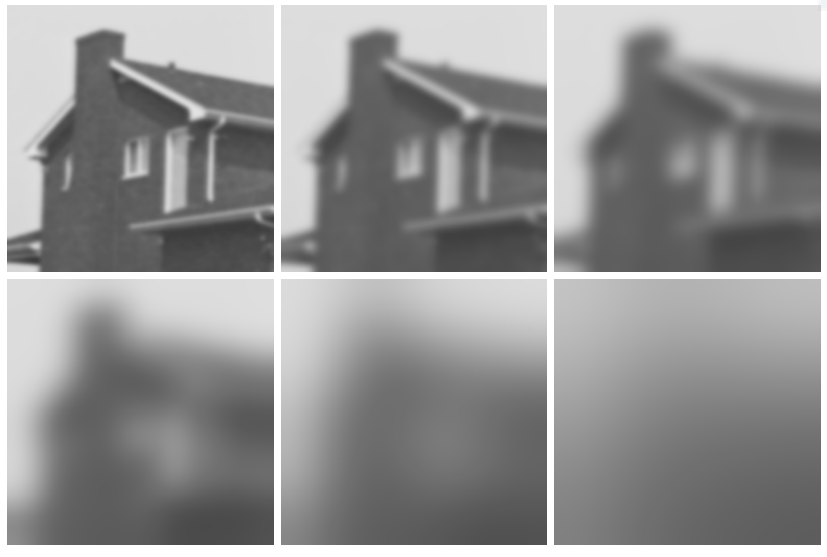
\includegraphics[scale=0.5]{assets/edge_detection_smoothing.png}
  
  Smoothing with $\sigma = 2,4,8,16,32,64$
  
  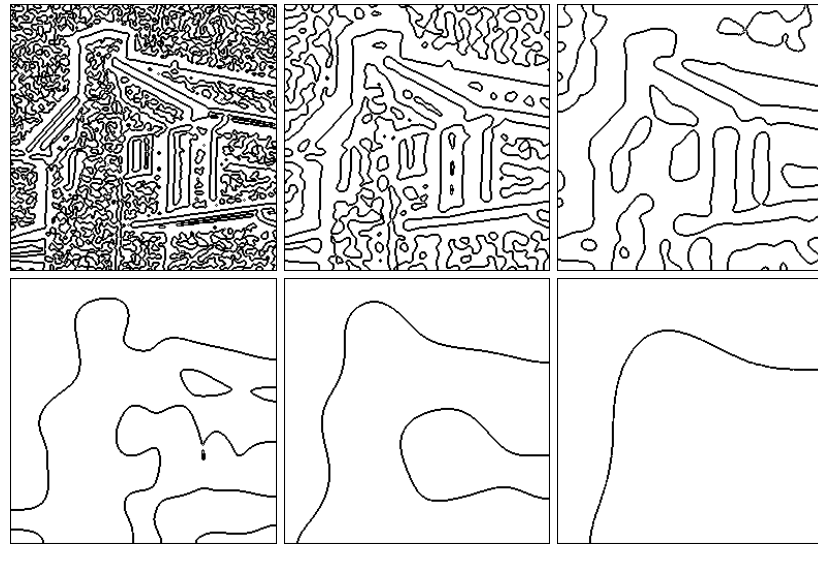
\includegraphics[scale=0.5]{assets/edge_detection_second_derivative.png}
  
  Zero crossings of the Laplacian
\end{center}

\paragraph{Advantages:}
\begin{enumerate}
  \item Closed contours with minimal width.
  \item No additional parameters beside the scale parameter $\sigma$ of the Gaussian.
\end{enumerate}

\paragraph{Disadvantages:}
\begin{enumerate}
  \item False alarms: It does not only detect maxima of the first derivative, but also local minima.
  \item Second-order derivatives are significantly more sensitive to high-frequency noise than first-order derivatives.
  \item Usually strong smoothing is required, leading to incorrect edge location shifts.
\end{enumerate}

\paragraph{Interesting Observations on Causality:}
\begin{itemize}
  \item Structures that can be located at a large scale $\sigma$ can be traced back to finer scales to localize them better. This property is known as \textbf{causality}.
  \item This introduces the concept of \textbf{scale-space}: embedding an image into a continuous family of increasingly smoothed versions of itself.
\end{itemize}



---

\subsubsection{Edges in Multichannel Images}
\paragraph{Basics From Linear Algebra:} The following is needed to understand the logic for Multichannel Images and Corner Detection.

Let $A \in \mathbb{R}^{n\times n}$. If there exists a number $\lambda$ and a vector $v \in \mathbb{R}^n$ ($v \neq 0$) satisfying $Av = \lambda v$, then $\lambda$ is an \textbf{eigenvalue} of $A$ with its associated \textbf{eigenvector} $v$. 

If some eigenvalue is known, then every nontrivial solution $v$ of $(A-\lambda I)v = 0$ is an eigenvector. Usually, the length of the eigenvector is normalized to $1$ ($\|v\|_2 = 1$). Eigenvalues can be computed as zeroes of the \textbf{characteristic polynomial}:
\[ p(\lambda) := \det(A-\lambda I) \]

If $A$ is symmetric, then all $n$ eigenvalues of $A$ are real numbers, and one can find $n$ eigenvectors that form an orthonormal basis of $\mathbb{R}^n$. If a symmetric matrix has only positive eigenvalues ($\lambda_i > 0$), it is called \textbf{positive definite} (or \textbf{positive semidefinite} for nonnegative eigenvalues, $\lambda_i \geq 0$).

If $A$ is symmetric, then $Q(x) = x^TAx$ forms a quadratic form. Out of all vectors $x \in \mathbb{R}^n$ with a specified unit length, $Q(x)$ is maximized or minimized by the eigenvector corresponding to the largest or smallest eigenvalue, respectively.

\paragraph{Applying Canny's Method to Multichannel Images:}
\begin{enumerate}
  \item Presmoothing an image $f = (f_1,\dots,f_m)^T$ with $m$ channels by componentwise convolution with a Gaussian $K_\sigma$ gives us the smoothed vector $u = (u_1,\dots,u_m)^T$. Each channel is smoothed separately.
  \item Define the \textbf{joint edge magnitude} as the Euclidean length of the individual gradient magnitudes vector $(|\nabla u_1|,\dots,|\nabla u_m|)^T$:
  \[ \sqrt{|\nabla u_1|^2 + \dots + |\nabla u_m|^2} \]
  \item For Non-maxima suppression, we need a definition for the \textbf{joint gradient direction} of a multichannel image. How do we define it?
  
  Summing the gradients of all channels directly is a bad idea because opposing channels can nullify each other. The gradient direction must be considered, but not its orientation (sign). See the method below.
  
  \item For Hysteresis thresholding, we require this calculated joint edge magnitude.
\end{enumerate}

\begin{center}
  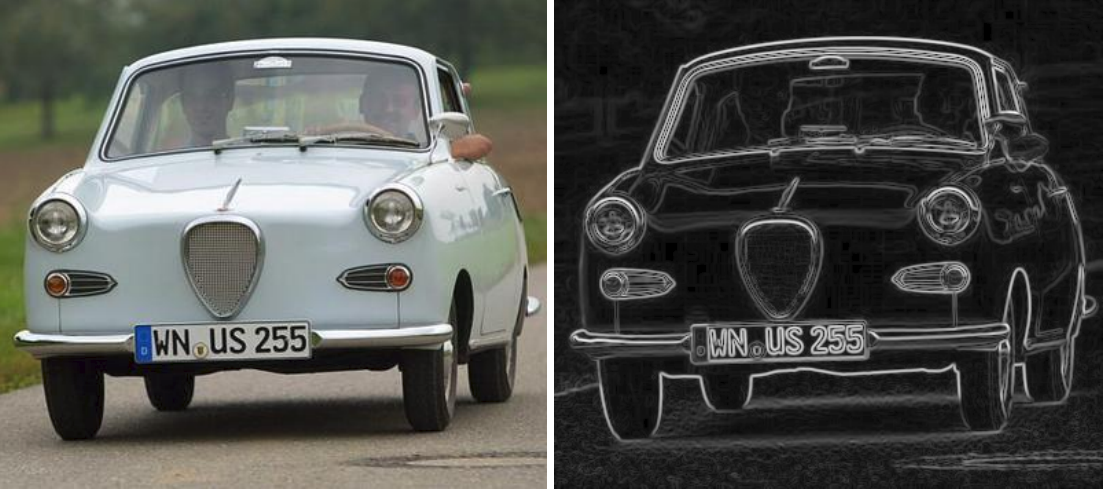
\includegraphics[scale=0.5]{assets/edge_detection_multichannel.png}
\end{center}

\paragraph{Di Zenzo's Method for Joint Edge Direction:}
The Gradient direction of a multichannel image $u = (u_1,\dots,u_m)^T$ is defined as the unit vector $n$ that is 'most parallel' to the channel gradients $\nabla u_1,\dots,\nabla u_m$. It maximizes the energy functional:
\[ E(n) := \sum_{i=1}^m (n^T \nabla u_i)^2 \]
This ensures only the direction of $\nabla u_i$ matters, not the orientation. Since $n^T\nabla u_i = \nabla u_i^Tn$, we can rewrite this expression as:
\[ E(n) = \sum_{i=1}^m n^T \nabla u_i \nabla u_i^T n = n^T \left( \sum_{i=1}^m \nabla u_i \nabla u_i^T \right) n \]

This is a quadratic form with the symmetric matrix $J$:
\[ J := \sum_{i=1}^m \nabla u_i \nabla u_i^T = \begin{pmatrix}
  \sum_{i=1}^m u_{ix}^2 & \sum_{i=1}^m u_{ix}u_{iy} \\
  \sum_{i=1}^m u_{ix}u_{iy} & \sum_{i=1}^m u_{iy}^2
\end{pmatrix} \]
And it is maximized if $n$ is chosen as the eigenvector corresponding to the largest eigenvalue of $J$.

\paragraph{How to Compute the Eigenvector:}
\begin{itemize}
  \item The system $Jv = \lambda v$ gives us $(J - \lambda I)v = 0$.
  \item Since an eigenvector is never $0$, the matrix $(J - \lambda I)$ must be singular ($\det(J - \lambda I) = 0$):
  \[ 0 = (j_{11} - \lambda)(j_{22} - \lambda) - j_{12}^2 \]
  \item Solving this quadratic equation in $\lambda$ yields the two eigenvalues:
  \[ \lambda_1 = \frac{1}{2}\left(j_{11} + j_{22} + \sqrt{(j_{11} - j_{22})^2 + 4j_{12}^2}\right) \]
  \[ \lambda_2 = \frac{1}{2}\left(j_{11} + j_{22} - \sqrt{(j_{11} - j_{22})^2 + 4j_{12}^2}\right) \]
  \item We only need the larger eigenvalue $\lambda_1$ to maximize our quadratic form.
\end{itemize}

\begin{center}
  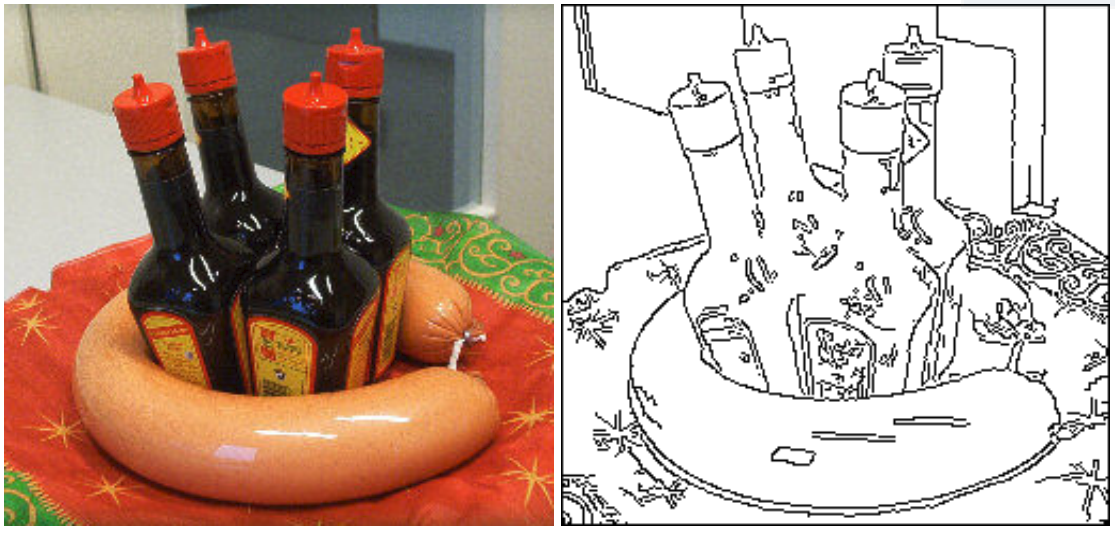
\includegraphics[scale=0.5]{assets/canny_edge_detector_multichannel.png}
\end{center}

---

\subsubsection{The Structure Tensor}
We are now back to working on grayscale images, trying to identify corners. The local structure direction around a corner changes strongly, which requires us to integrate directional information over a spatial neighborhood.

We cannot just average gradients because they can cancel each other out. The solution is to average the structure direction within some spatial neighborhood $B_\rho(x,y)$ of radius $\rho$ around point $(x,y)$. This is a similar strategy to multichannel images, using spatial averaging instead of channel averaging:
\[\begin{split}
E(n) &:= \int_{B_\rho(x,y)} (n^T\nabla u)^2 \, dx' \, dy' \\
&= \int_{B_\rho(x,y)} n^T \nabla u(x',y') \nabla u^T(x',y') n \, dx' \, dy' \\
&= n^T \left( \int_{B_\rho(x,y)} \nabla u(x',y') \nabla u^T(x',y') \, dx' \, dy' \right) n
\end{split}\]

The optimal $n$ is the normalized eigenvector to the largest eigenvalue of that spatial integral matrix. 

Right now, this neighborhood window averages with equal weight. We can replace this hard boundary box with a smooth Gaussian window using a Gaussian convolution:
\[ J_\rho(\nabla u) := K_\rho \ast (\nabla u \nabla u^T) = \begin{pmatrix}
  K_\rho \ast (u_x^2) & K_\rho \ast (u_x u_y) \\
  K_\rho \ast (u_x u_y) & K_\rho \ast (u_y^2)
\end{pmatrix} \]

This matrix $J_\rho$ is called the \textbf{structure tensor} (or second-moment matrix). It is symmetric and positive semidefinite. Its orthonormal eigenvectors $v_1, v_2$ specify the preferred structure directions within the integration scale $\rho$. Their eigenvalues describe the average contrast along these directions. 

We can analyze local image features using these eigenvalues ($\lambda_1 \geq \lambda_2$):
\begin{itemize}
  \item \textbf{Constant area:} $\lambda_1 = \lambda_2 = 0$ (no gradient)
  \item \textbf{Straight edges:} $\lambda_1 \gg \lambda_2 = 0$ (strong gradient in one direction)
  \item \textbf{Corners / Junctions:} $\lambda_1 \geq \lambda_2 \gg 0$ (strong gradients in multiple directions)
  \item \textbf{Measure of anisotropy:} $(\lambda_1 - \lambda_2)^2$
\end{itemize}



---

\subsubsection{Corner Detection with First Order Derivatives}
It is based on the structure tensor. If we consider the Gaussian-smoothed version of the original image $f$ and compute the structure tensor:
\[ J_\rho(\nabla u) = K_\rho \ast (\nabla u \nabla u^T) \]
In corners, the gradient direction changes rapidly within its neighborhood. The integration scale $\rho$ should be selected to be larger than the initial noise scale $\sigma$. In these corner configurations, the structure tensor yields two large eigenvalues: $\lambda_1 \geq \lambda_2 \gg 0$.

\paragraph{Most Popular Structure Tensor Based Corner Detectors:} Let $\text{local max}$ denote a spatial local maximum search, and assuming $\lambda_1 \geq \lambda_2$:

\begin{itemize}
  \item \textbf{Tomasi/Kanade:}
  \[ \lambda_2 > T \quad \text{and} \quad \lambda_2 = \text{local max} \]
  Simple concept, but explicitly requires computing the smaller eigenvalue $\lambda_2$.
  
  \item \textbf{Rohr:}
  \[ \det J_\rho = j_{11}j_{22} - j_{12}^2 > T \quad \text{and} \quad \det J_\rho = \text{local max} \]
  Since $\det J_\rho = \lambda_1\lambda_2$, both eigenvalues must be large to pass the threshold. It avoids direct eigenvalue extraction.
  
  \item \textbf{Förstner / Harris:}
  \[ \text{tr} J_\rho = j_{11} + j_{22} > T \quad \text{and} \quad \frac{\det J_\rho}{\text{tr} J_\rho} = \text{local max} \]
  Since $\text{tr} J_\rho = \lambda_1 + \lambda_2$, both eigenvalues are balanced against each other. It completely bypasses eigenvalue roots computation.
\end{itemize}

\begin{center}
  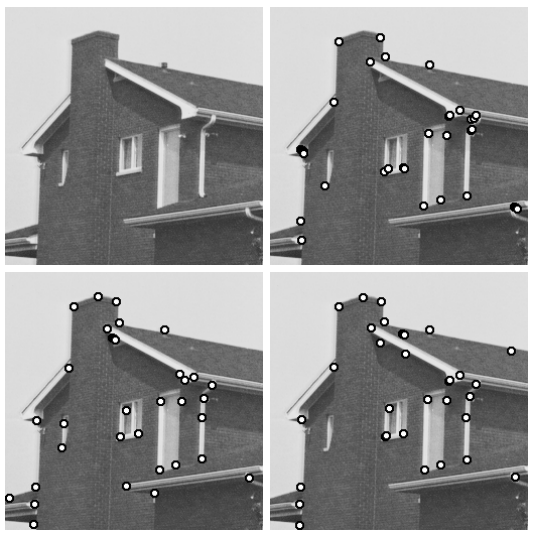
\includegraphics[scale=0.5]{assets/corner_detection.png}
  \begin{itemize}
    \item Top-right: Tomasi with $T=18.2$
    \item Bottom-left: Rohr with $T=100$
    \item Bottom-right: Förstner with $T=72$
  \end{itemize}
\end{center}
TODO:Second derivative corner detection
\section{Nonlinear Filters}
\subsection{Morphological Filters}
They are based on \textbf{mathematical morphology}, that analyzes the shape of objects in an image.
\subsubsection{Properties of Basic Morphological Filters}
They are invariant under monotonically increasing greyscale transformations.
\[MGf = GMf\]
for any image $f$, any \textbf{basic} morphological filter $M$ and any monotonically increasing grayscale transform $G$.

There are four basic filters
\begin{enumerate}
  \item Erosion
  \item Dilation
  \item Opening
  \item Closing
\end{enumerate}
Stuff like brightness, and sensor characteristic don't matter. Image contrast does not matter as well.

Morphological methods only take into account the level sets.
\[L_i(f) = \{(x,y) | f(x,y) \geq i\}\]
\subsubsection{Dilation and Erosion}
Dilation replaces the gray value of a continuous image $f(x,y)$ by its supremum within a mask B
\[(f \oplus B)(x,y) := \sup \{f(x-x',y-y') | (x',y') \in B\}\]

Erosion is the opposite, using the infimum
\[(f \ominus B)(x,y) := \inf \{f(x+x',y+y') | (x',y') \in B\}\]
For discrete images we use maximum/minimum instead of supremum.

The mask B is called \textbf{structuring element}. Often convex structuring elements are used, disks or squares.

For binary images with bright object and dark background, dilation propagates contour into the outside, erosion movies it to the outside.

\begin{center}
  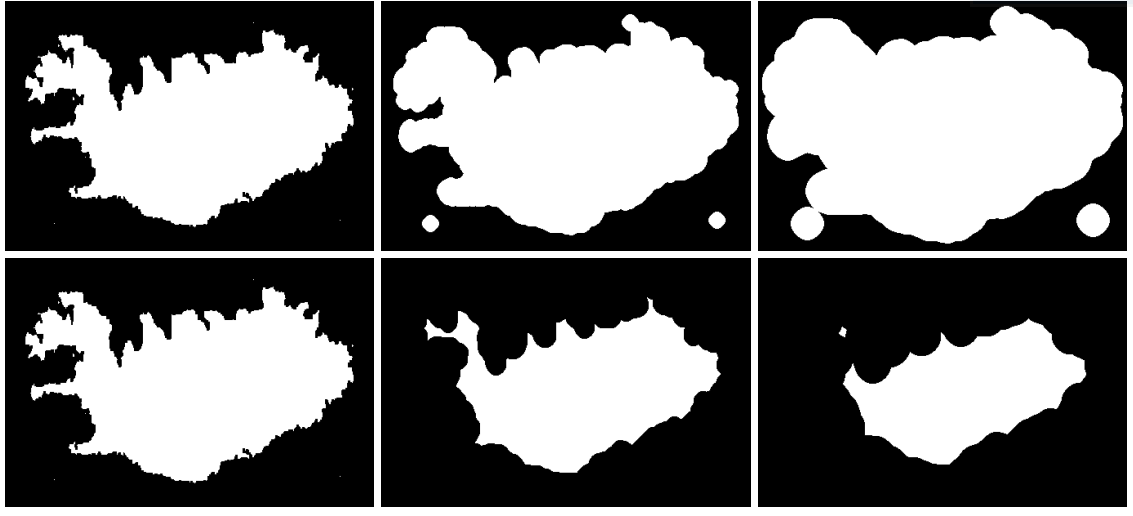
\includegraphics[scale=0.4]{assets/dilation_erosion.png}
  
  Dilation on top, erosion on the bottom.
\end{center}
\paragraph{Algorithms for Conex Structuring elements}: The good thing is that convex structuring elements are \textbf{scalable}, meaning one dilation/erosion with structure $nB$ is the same as n dilation/erosion with structure $B$. This scalability is important

\paragraph{Algorithms for rectangular strucuring elements}: Rectangular structuring elements are separable.

\subsubsection{Morphological Lowpass Filters: Opening and Closing}
\paragraph{Closing}: The goal is to simplify image structure but avoid the expansion of dilation.
\[f \bullet B := (f \oplus B) \ominus B\]
It closes gaps in bright structures by removing dark details

$f \bullet B$ can be brighter than $f$, and it acts as a morphologicall lowpass filter with regard to dark details

\paragraph{Opening}: The goal is to simplify the image but avoid shrinkage of erosion
\[f \circ B := (f \ominus B) \oplus B\]
It closes gaps in dark structures by removing bright details, and it acts as a morphologicall lowpass filter with regard to bright details

$f \circ B$ can be darker than $f$

\subsubsection{Morphological Bandpass Filters: Granulometries}
Multiple openings and closings with the same $B$ do no alter the image any more (idempotency)
\[(f \circ B) \circ B = f \circ B\]
\[(f \bullet B) \bullet B = f \bullet B\]

Openings and closings are called \textbf{sieve operations}. Structures that pass the sieve once will also pass it a second time.

Using structuring elements of increasing size, can make so that we first remove small, then middle, and then coarse scale structures step by step.  This is called \textbf{granulometry}. Each image in a granulometry is the difference between subsequent images in a chain of openings or closings with structuring elements of increasing size (similar to Laplacian Pyramids \ref{subsec:laplacian-pyramid})

They play the role of morphological bandpass filters

\subsubsection{Morphological Highpass Filters: Top Hats}
They extract fine-scale details
\paragraph{White Top Hats}: The opening $f\circ B$ removes bright details. So we inverse it to get the details
\[WTH(f) := f - (f\circ B)\]
This definition guarantees non-negative results

\paragraph{Black Top Hats}: Same but with Closings
\[BTH(f) := f - (f\bullet B)\]
Also guarantee of nonnegativity in the result.

\paragraph{Selfdual Top Hat}: To extract both details
\[\rho(f) = WTH(f) + BTH(f) = (f\bullet B) - (f\circ B)\]

With $\rho(f)$ being invariant to grayscale inversion
\subsection{Median Filters}
The goal is to remove noise that creates impulse-like outliers (e.g Salt and Pepper noise \ref{itm:salt-pepper-noise})

This is done by taking all the gray values in a $(2m+1)\times (2m+1)$ mask, and order them and taking the median. This type of filter belongs in the \textbf{rank order filters}

\begin{center}
  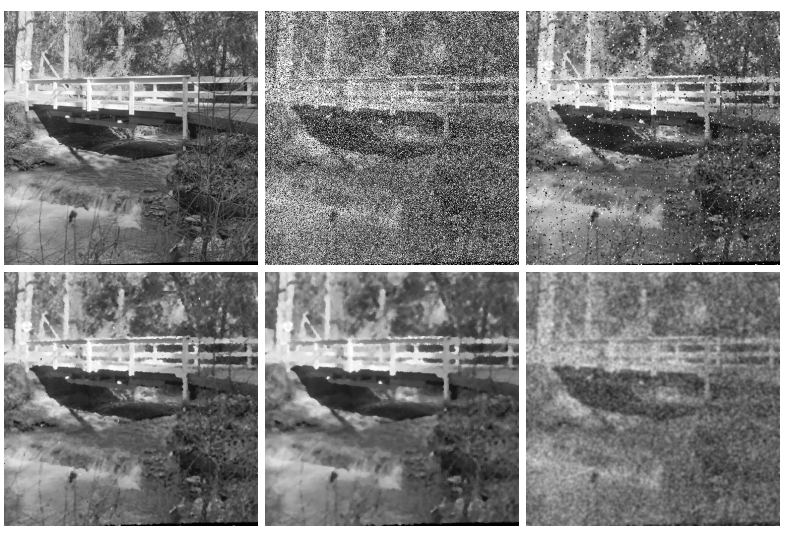
\includegraphics[scale=0.5]{assets/median_filter.png}
  \begin{itemize}
    \item Top Left: Original image
    \item Top: 40\% salt and pepper noise
    \item Top right: $3\times 3$ median filtering. Works pretty well
    \item Bottom left: $5\times 5$ median filtering, good but looks a bit funky
    \item Bottom: $7\times 7$ median filtering, quite a lot of detail is lost.
    \item Bottom right: Gaussian filtering $\sigma = 3$, works really badly.
  \end{itemize}
\end{center}

\paragraph{Properties}
\begin{itemize}
  \item They are also morphological filters, keep the original invariance
  \item Good to remove impulse noise
  \item Preserves (straight) edges better than linear filters
  \item Leads to rounding of corners
  \item Often stabilises after a few iterations to a \textbf{root singal}, can also oscillate though
  \item Not separable
  \item Sorting can be time-consuming for large masks.
\end{itemize}


\subsection{Wavelet Shrinkage}
Three step procedure
\begin{enumerate}
  \item Analysis Step: Represent image in wavelet basis. You hope that most of your signal is in the large wave coefficients.
  \item Shrinkage Step: Shrink wavelet coefficients with small magnitude towards 0. (\textbf{Don't shrin the scaling coefficient})
  \item Synthesis Step: Reconstruct the image
\end{enumerate}
Similar to image compression with wavelets, which we already saw. Very fast

\subsubsection{Shrinking Strategies}
Let $I_a$ be an indicator function that returns $1$ if $a$ is true, $0$ if false


\begin{center}
  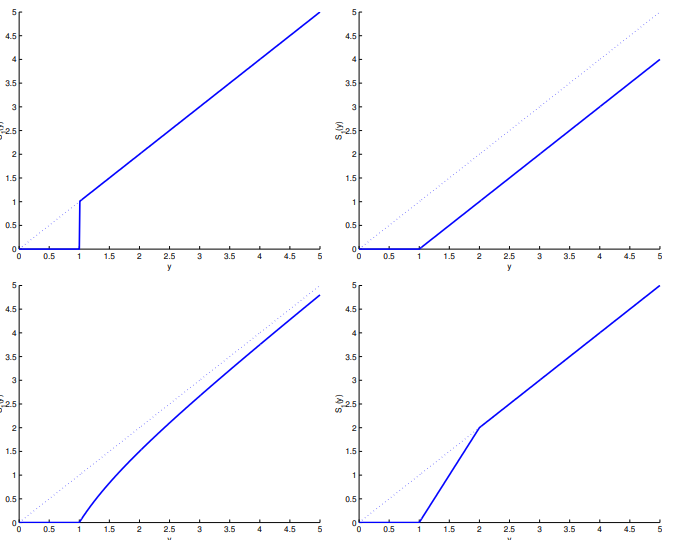
\includegraphics[scale=0.5]{assets/wavelet_shrinkage.png}
\end{center}
\begin{itemize}
  \item Hard Shrinkage (Top Left):
  \[S_T(s) := s I_{\{ |s| > T\}}\]
  Everything below a threshold is set to zero, the rest stays the same
  \item Soft Shrinkage (Top Right):
  \[S_T(s) := sgn(s) (|s|-T)I_{\{|s| > T\}}\]
  Shrink everything, but forces the values under the threshold to zero.
  \item Garrote Shrinage (Bottom Left):
  \[S_T(s) := \left(s - \frac{T^2}{s}\right)I_{\{|s|>T\}}\]
  \item Semisoft Shrinkage (Firm Shrinkage) (Bottom Right):
  \[S_{T_1,T_2}(s) := \begin{cases}
    0 & |S| \leq T_1\\
    sgn(s) \frac{T_2(|s|-T_1)}{T_2-T_1} & T_1 < |S| \leq T_2 \\
    s & |s| > T_2
  \end{cases}\]
\end{itemize}
\subsubsection{Why does it work better with edges than linear filtering?}
The impact of a single wavelet coefficient is \textbf{local}, instead of each Fourier coefficient, which is \textbf{global}. Because edges create wavelet coefficients with large magnitude, they are not that influenced under shrinkage.

\subsubsection{Properties}
\begin{itemize}
  \item It does not affect the average gray value, the wavelet has mean 0, shrinking doesn't affect that.
  \item What can happen, is that the maximum gray value increases and the minimum gray value decreases. In some scenario, this appears very often.
  \item Usual wavelet shrinkage is not shift invariant and not invariant under rotations
\end{itemize}
\subsubsection{Shift-Invariant Wavelet Shrinkage}
Averaging over all possible translations creates shift-invariant wavelet shrinkage. (\textbf{cycle spinning})


\subsection{Bilateral Filtering}
It's an adaptive averaging with weights that
\begin{itemize}
  \item decrease with increasing distance from stencil center
  \[\text{Spatial weights } w(|x_i-x_j|^2)\]
  \item decrease with increasing disance of the grey values (preserves edges)
  \[\text{Tonal weights }g(|f_i-f_j|^2)\]
\end{itemize}

Computes filtered signal u of f via
\[u_i = \frac{\sum_j g(|f_i-f_j|^2) w(|x_i-x_j|^2)f_j}{\sum_j g(|f_i-f_j|^2)w(|x_i-x_j|^2)}\]

with decreasing nonnegative functions w and g. They usually are Gaussians with standard deviation $\sigma_s$ and $\sigma_t$
\subsubsection{Properties}
\begin{itemize}
  \item Shift-invariant and invariant under rotation
  \item Gives results with good quality
  \item No over-under shoots
  \[\min_i f_i \leq u_j \leq \max_i f_i \quad \forall j\]
  \item Can be iterated
  \item Slower than wavelet shrinkage
  \item Does not preserve average gray value
  \item Requires two parameters $\sigma_s ,\, \sigma_t$ to be specified
  \item Fairly popular in computer graphics
\end{itemize}
\subsection{NL-Means}
Adaptive averaging of pixels that belong to similar patches within entire image.

We call $N_i$ a square-shaped neighborhood of size $(2m+1) \times (2m+1)$ around a pixel i.

The gray value distance between two neighborhoods is (with $f(N)$ returning a vector, and then doing the Euclidean Distance)
\[|f(N_i) - f(N_j)|\]

The nonlocal(NL) means algorithm does weighted averaging, where more similar patches have higher weights
\[u_i = \frac{\sum_j g(|f(N_i) - f(N_j)|)f_j}{\sum_j g(|f(N_i) - f(N_j)|)}\]
Often a Gaussian is used as weight function $g$
\begin{center}
  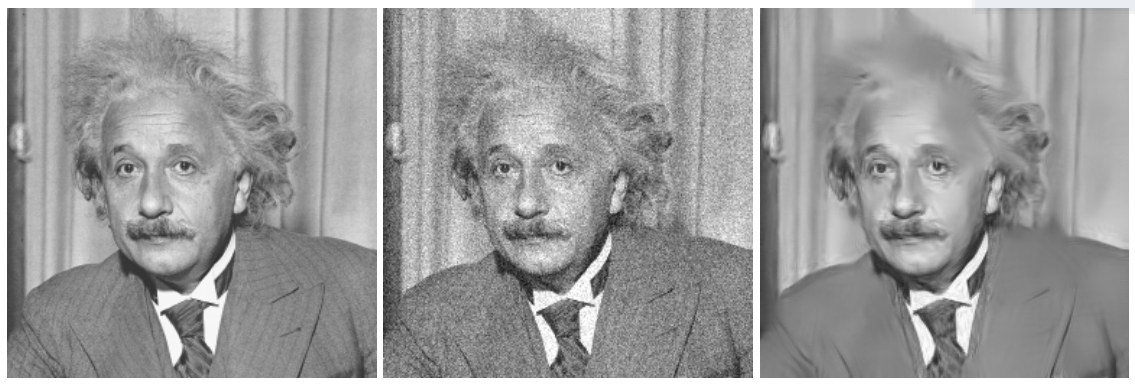
\includegraphics[scale=0.5]{assets/nl_means.png}

  Original image, gaussian noise, NL means
\end{center}
\subsubsection{Properties}
\begin{itemize}
  \item Can give high-quality results
  \item Satisfies the same max-min principle of before
  \item Shift invariant
  \item Not rotationally invariant for square-shaped patches
  \item Does not preserve average gray value
  \item Pretty slow. Usually search space is restricted
  \item Three parameters: neighborhood, search space and Gaussian standard deviation
\end{itemize}

\subsection{Nonlinear Diffusion Filtering}
\subsubsection{Motivation}
They are denoising methods that have some extra advantages
\begin{itemize}
  \item Smooth within a region and preserve edges (in contrast to shift-invariant linear filters)
  \item Preserve average gray value (over bilateral filters and NL means)
  \item Are invariant under shifts and do not over/under shoot (in contrast to classical wavelet shrinkage)
  \item Can be designed flexibly
\end{itemize}

They obviously have their own limitations
\begin{itemize}
  \item Slower than linear and morphological filters
\end{itemize}

\subsubsection{Mathematical Background}
\paragraph{Partial Derivatives}: For a sufficiently smooth function of several variables, one can compute it's partial derivative. As is known, you derivate with respect to that variable and the rest are treated like constants.

\[f(x,y) = \sin(xy^2) + x^3\]
\[\frac{\partial f}{\partial x}(x,y) = y^2 \cos(xy^2) + 3x^2\]
Under some smoothness assumptions we can exchange the order of differentiation
\[f_{xy} = f_{yx}\]
\paragraph{Nabla Operator}: It is the \textbf{gradient}
\[\nabla := \begin{pmatrix}
  \partial_x \\
  \partial_y
\end{pmatrix}\]
You can usually treat it as a vector
\[\nabla f = \begin{pmatrix}
  \partial_x f \\
  \partial_y f
\end{pmatrix}\]
With $\nabla f $ points in the direction of the steepest ascent of $f$

\paragraph{Divergence and Laplacian}: The inner product of the nabla operator and the vector-valued function $j(x,y) = (j_1(x,y),j_2(x,y))^T$ is called the \textbf{divergence} of $j$.

\[div\, j := \nabla^t j = (\partial_x, \partial_y)\begin{pmatrix}
  j_1 \\
  j_2
\end{pmatrix} = \partial_x j_1 + \partial_y j_2\]

And the inner product of the divergence and the gradient is called the \textbf{Laplacian} (Laplace-operator)
\[\Delta f := div (\nabla f) = \partial_{xx}f + \partial_{yy}f\]

\paragraph{Partial Differential Equations (PDEs)}: An \textbf{algebraic equation} relates an unknown number with its powers. Example:
\[x^2 - 8x + 15 = 0\]

\textbf{Differential equations} state relation between unknown function and its derivatives
\[\frac{du(t)}{dt} = 5u(t)\]
and if we specify an initial condition such as $u(t=0) = 2$ we can get a unique solution
\[u(t) = 2e^{5t}\]
If $u$ depends on one variable $t$ we have ordinary derivatives / ordinary differential equations.

If u is a function of multiple variables, partial derivatives may appear. Then we have \textbf{partial differential equations}

\subsubsection{What is diffusion?}
Diffusion equilibrates concentration differences by redistributing mass. It preserves the total mass

(Isotropic) diffusion are described by the PDE
\[\partial_t u = div(g\cdot \nabla u)\]
where the divergence and nabla operator involve only spatial derivatives, not the temporal ones.

The longer the diffusion time $t$, the more the differences are equilibrated.

Diffusivity $g$ may depend on location. Locations where $g$ is larger, diffusion goes faster.

\subsubsection{Continuous Diffusion Filter}
The image domain is a rectangular domain $\Omega:= (0,a_1 )\times (0,a_2)$

The image is a bounded function $f:\Omega \to \mathbb{R}$


We compute a filtered version $u(x,y,t)$ of $f(x,y)$ as solution of the diffusion equation
\[\partial_y u = div(g \nabla u)\]
with the original image as the initial condition
\[u(x,y,0) = f(x,y)\]
and reflecting boundary conditions
\[\partial_n u = 0\]
with $n$: unit normal vector at image boundary $\partial \Omega$ and $\partial_n u :=n^T\nabla u$
\paragraph{Diffusivity Choice}: We want to reduce diffusion at edges in order to preserve them.

$|\nabla u| = \sqrt{u_x^2 +  u_y^2}$ is a reasonable indicator for an edge. Edges are where $|\nabla u |$ is large.

So knowing that, we pick a diffusivity based on that, e.g the \textbf{Charbonnier diffusivity}
\[g(|\nabla u|) := \frac{1}{\sqrt{1 + |\nabla u|^2 / \lambda^2}}\]

or the faster-decreasing \textbf{Perona-Malik diffusivity}
\[g(|\nabla u| := \frac{1}{1+ |\nabla u|^2 \lambda^2})\]

The positive parameter $\lambda$ serves as \textbf{contrast parameter}. Location where $|\nabla u| > \lambda$ are regarded as edges, and diffusivity is reduced significantly
\begin{center}
  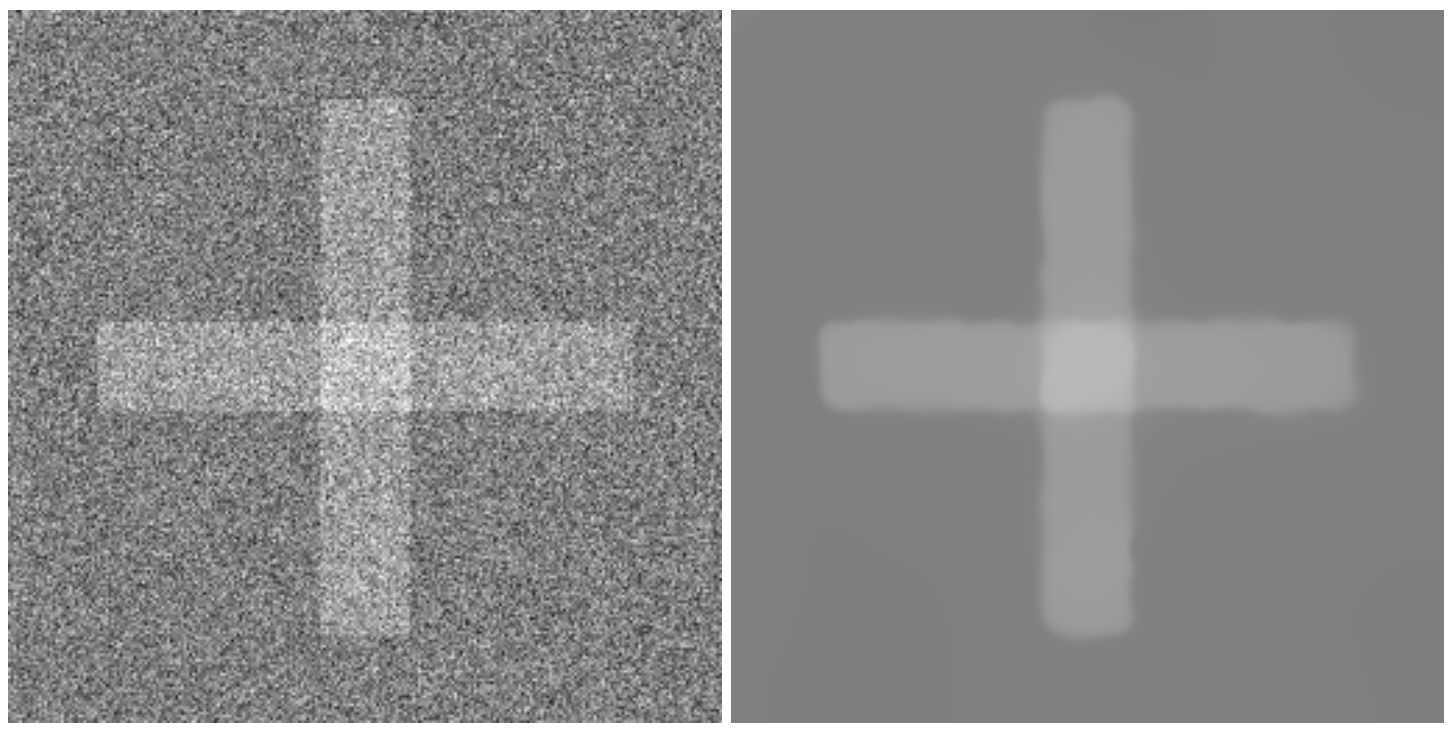
\includegraphics[scale=0.3]{assets/continuous_diffusion_filter.png}

  Effect of Charbonnier diffusivity with $\lambda = 0.1$ and $t=500$
\end{center}

\subsubsection{A simple algorithm}
\paragraph{Finite Difference Approximation}: We can rewrite the continuous diffusion equation as
\[\partial_t u = \partial_x \left(g(|\nabla u|)\partial_x u\right)+ \partial_y \left(g(|\nabla u|)\partial_y u\right)\]
and approximations in $\left((i-1/2)h_1,(j-1/2)h_2, k \tau\right)$ are given by

\[u\approx u_{i,j}^k\]
\[\partial_t u \approx \frac{u_{i,j}^{k+1} - u_{i,j}^k}{\tau}\]
\[\partial_x(g\partial_x u) \approx \frac{1}{h_1} \left((g\partial_x u)^k_{i+1/2,j} - (g\partial_x u)^k_{i-1/2,j}\right) \]
\[\approx \frac{1}{h_1}\left(g_{i+1/2,k}^k \frac{u_{i+1,k}^k - u_{i,j}^k}{h_1}-g_{i-1/2,j}^k \frac{u_{i,j}^k - u_{i-1,j}^k}{h_1}\right)\]

with spatial grid sizes $h_1$,$h_2$ and time step size $ \tau$

The diffusivity approximations at the set positions can be computed as the arithmetic mean
\[g_{i+1/2,j}^k \approx \frac{g_{i,j}^k + g_{i+1,j}^k}{2}\]

And the diffusivity $g_{i,j}^k$ at the grid position $i$, $j$ and step $k$ can be computed as
\[g_{i,j}^k = g\left(\sqrt{(\partial_x u)^2 + (\partial_y u)^2}\right)|_{i,j}^k\]
\[\approx g\left( \sqrt{\left(\frac{u_{i+1,j}^k - u_{i-1,j}^k}{2h_1}\right)^2 + \left(\frac{u_{i,j+1}^k - u_{i,j-1}^k}{2h_2}\right)^2}\right)\]

So the resulting numerical scheme is
\[\frac{u_{i,j}^{k+1} - u_{i,j}^k}{\tau} = \frac{1}{h_1}\left(g_{i+1/2,j}^k \frac{u_{i+1,j}^k - u_{i,j}^k}{h_1} - g_{i-1/2,j}^k \frac{u_{i,j}^k - u_{i-1,j}^k}{h_1}\right)\]
\[ + \frac{1}{h_2}\left(g_{i,j+1/2}^k \frac{u_{i,j+1}^k - u_{i,j}^k}{h_2} - g_{i,j-1/2}^k \frac{u_{i,j}^k - u_{i,j-1}^k}{h_2}\right)\]

So based on that, we are able to compute $u_{i,j}^{k+1}$ explicitly from known values at time step $k$

\[u_{i,j}^{k+1} = u_{i,j}^k + \frac{\tau}{h_1}\left(g_{i+1/2,j}^k \frac{u_{i+1,j}^k - u_{i,j}^k}{h_1} - g_{i-1/2,j}^k \frac{u_{i,j}^k - u_{i-1,j}^k}{h_1}\right)\]
\[+ \frac{\tau}{h_2}\left(g_{i,j+1/2}^k \frac{u_{i,j+1}^k - u_{i,j}^k}{h_2} - g_{i,j-1/2}^k \frac{u_{i,j}^k - u_{i,j-1}^k}{h_2}\right)\]

This scheme is called an \textbf{explicit scheme}


And this explicit scheme can be rewritten as weighted averaging
\begin{center}
  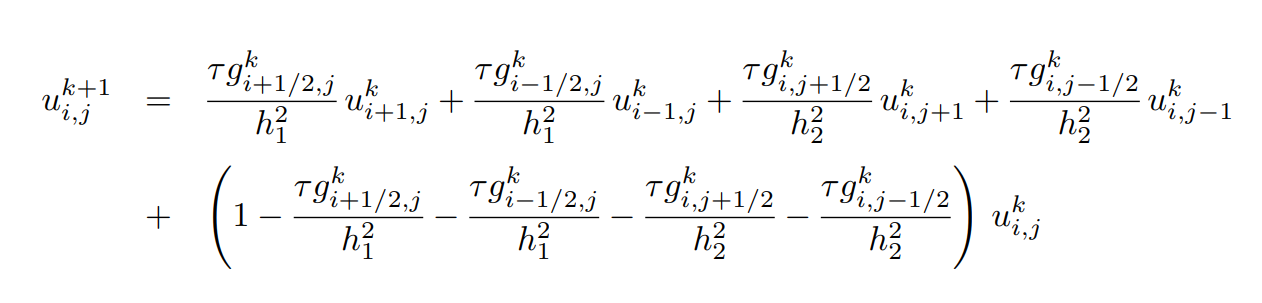
\includegraphics[scale=0.3]{assets/a_simple_algorithm.png}
\end{center}
At the image borders we add an additional one-pixel layer by mirroring to ensure reflecting boundary conditions

\paragraph{Stencil notation}: This if for $h_1 = h_2 = 1$
\begin{center}
  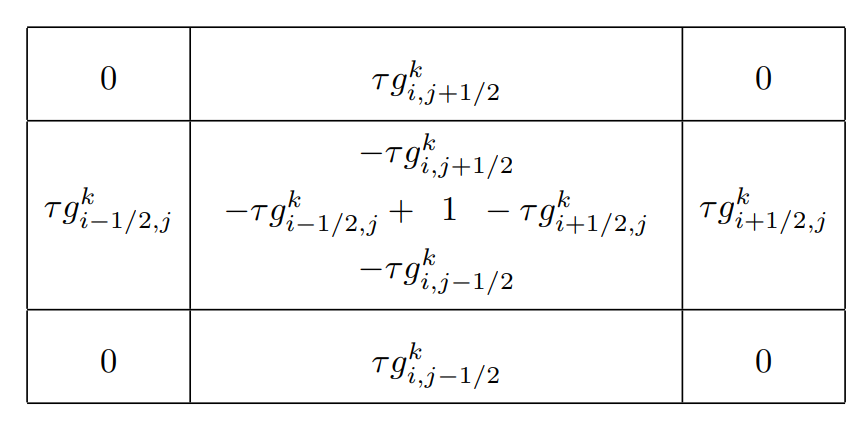
\includegraphics[scale=0.3]{assets/a_simple_algorithm_2.png}
\end{center}

Space-time dependent averaging where the weights sum up to one.

Central weight becomes negative if $\tau$ is too large. This leads to instability

For $|g| \leq 1$ we get stable convex combination if $\tau \leq 0.25$. In this case, no over or undershoots are possible 

\paragraph{Comparison to Bilateral Filtering}

it is similar in the sense that
\begin{itemize}
  \item Result looks similar
  \item Diffusion time $t$ resembles spatial parameter $\sigma_s$
  \item Contrast parameter $\lambda$ resembles tonal parameter $\sigma_t$
\end{itemize}
Differences
\begin{itemize}
  \item Diffusion filtering iterates a small adaptive kernel, while bilateral filtering uses one large adaptive kernel
  \item Diffusion preserves average gray level, bilateral does not.
\end{itemize}
\section{Global Filters}
Until now, the image enhancement methods were either point operations or local methods (linear or non-linear)

Now we will use a \textbf{global} method, these are called \textbf{variational methods} or \textbf{regularisation methods}

\subsection{One-Dimensional Case}
We want image smoothing transformations that satisfies an optimality criterion.

The filtered image $u$ should be
\begin{itemize}
  \item Close to the original image $f$
  \item As smooth as possible
\end{itemize}
\subsubsection{Simple 1-D Approach}
We have 1-D signal $f=(f_1,...,f_N)^T$. The filtered signal $u=(u_1,..,u_N)^T$ as a minimiser of the \textbf{cost function (energy)}
\[E_f(u) := \frac{1}{2}\underbrace{\sum_{k=1}^N(u_k-f_k)^2}_{\text{similarity}}  + \frac{\alpha}{2}\underbrace{\sum_{k=1}^N(u_{k+1}-u_k)^2}_{\text{smoothness}}\]
There is a smoothness weight $\alpha > 0$ called the \textbf{regularisation parameter}. Larger values give smoother images. These methods with quadratic smoothness are called \textbf{Whittaker-Tikhonov regularisation}

\paragraph{Neccesary Conditions for a Minimum}: For a minimum, the partial derivatives with respect to $u_1,...,u_N$ must all vanish. So that $\frac{\partial E_f}{\partial u_i} = 0 \quad \forall i =1,...,N$

So you get the energy equation, derivate to zero on all signals, and you have a big system of equations to solve.

\begin{center}
  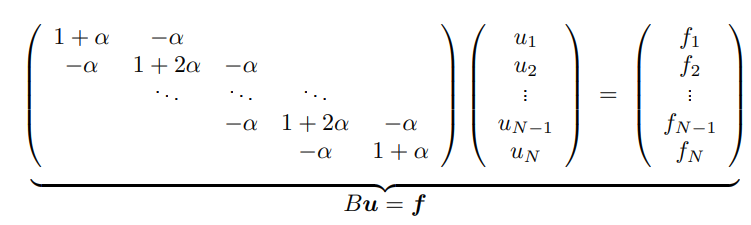
\includegraphics[scale=0.5]{assets/1_d_global_filter.png}
\end{center}

\paragraph{Properties}:
\begin{itemize}
  \item Image boundaries are treated correctly without any extra steps
  \item Smoothing can be fine tuned continously via $\alpha$
  \item The system matrix $B$ is \textbf{strictly diagonally dominant}, meaning
  \[|b_{ii}| > \sum_{j, i \neq i}|b_{j,i}| \quad \forall i\]
  This means that the matrix is invertible (Gershgorin's theorem). Also, it can be shown that $B^{-1}$ is a full matrix with positive entries only.
  \item Since the solution $u=B^{-1}f$ and $B^{-1}$ is a full matrix with positive entries only. This means that $u$ results from averaging $f$ over a mask that does not vanish within the entire signal length.
  \item These filters are called \textbf{IIR filters}: infinite impulse response. All pixels are used.
  \item Many of our previous convolutions were FIR filters: Finite Impulse Response
\end{itemize}

\paragraph{Is this solution really a global minimum?} Yes, because $E_f(u)$ is strictly convex in $u$, meaning that
\[E_f(\beta u + (1-\beta)v) \leq \beta E_f(u) + (1- \beta)E_f(v)\]
for all $0< \beta < 1$, and for all $u,v\in \mathbb{R}^N$, with $u\neq v$

then $E_f(u)$ has at most one extremum, and that is a minimum.

\subsubsection{Thomas Method for Tridiagonal Systems}
It's an algorithm for the Gaussian elimination of tridiagonal linear systems. This is, as seen above, used in 1-D problems.
\begin{center}
  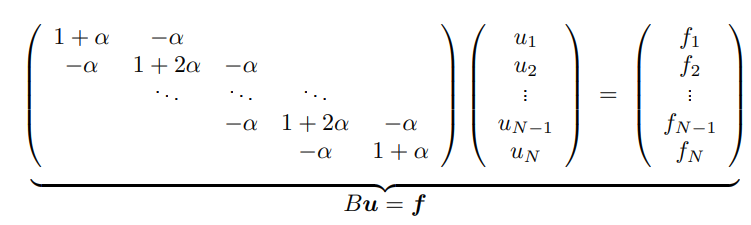
\includegraphics[scale=0.5]{assets/1_d_global_filter.png}
\end{center}
\paragraph{Algorithm}: We want to solve the linear system $Bu = f$ with
\begin{center}
  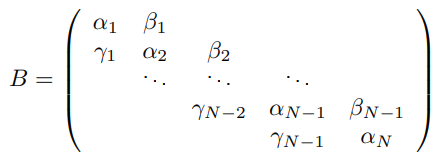
\includegraphics[scale=0.5]{assets/thomas_algorithm.png}
\end{center}
This is done in three steps
\begin{enumerate}
  \item LR Decomposition: $B=LR$ with lower bidiagonal matrix L and upper bidiagonal matrix R
  \begin{center}
    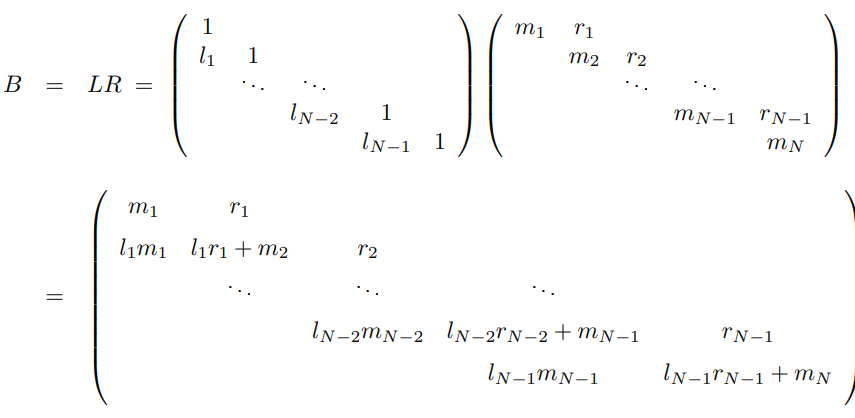
\includegraphics[scale=0.5]{assets/lr_decomposition.png}
  \end{center}
  So we can use this to get a simple algorithm to compute our desired coefficients
  \begin{algorithm}
    $m_1$ := $\alpha_1$ \\
    for $i=1,2,...,N-1${ \\
      $\quad l_i$ := $\gamma_i/m_i$\\
      $\quad m_{i+1}$ := $\alpha_{i+1} - l_i\beta_i$
    }
  \end{algorithm}
  And $r_i = \beta_i$ for $i=1,...,N-1$
  \item Forward elimination: Solve $Ly=f$ for $y$
  \begin{center}
    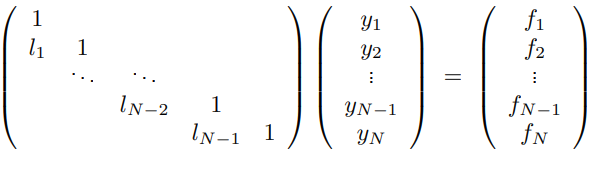
\includegraphics[scale=0.5]{assets/forward_elimination.png}
  \end{center}
  And we can use the following algorithm
  \begin{algorithm}
    $y_1$ := $f_1$ \\
    for $i = 2,3,...,N$: \\
    $\quad y_i$ := $f_i - l_{i-1}y_{i-1}$
  \end{algorithm}
  \item Backward substitution: Solve $Ru = y$ for $u$
  \begin{center}
    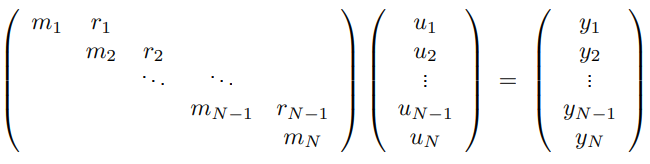
\includegraphics[scale=0.5]{assets/backward_substitution.png}
  \end{center}
   And similarly to forward elimination, we use an algorithm for the coefficients
  \begin{algorithm}
    $u_N$ := $y_N / m_B$ \\
    for $i = N-1,N-2,...,1$: \\
    $\quad u_i$ := $(y_i - \beta_iu_{i+1})/m_i$
  \end{algorithm}
  (we substituted $r_i$ with $\beta_i$ as seen above)
\end{enumerate}
\paragraph{Remarks}: 
\begin{itemize}
  \item The algorithm is stable for every strictly diagonally dominant system
  \item It is highly efficient, only needs $2N-1$ divisions, $3N-3$ multiplications and $3N-3$ subtractions. So it is $O(N)$
  \item Space complexity is also linear
  \item It is called \textbf{recursive filtering}
  \begin{itemize}
    \item Computation of filter coefficients
    \item Causal filter
    \item Anticausal filter
  \end{itemize}
\end{itemize}
\subsection{m-Dimensional Case}
Use a single index to count all pixels of an $m$-D image $f=(f_k)$. We define $\mathcal{N}(k)$ as the set of neighbours of pixel $k$

The m-dimensional energy is given
\[E_f(u) = \frac{1}{2}\sum_{k=1}^N(u_k - f_k)^2 + \frac{\alpha}{4}\sum_{k=1}^N\sum_{l\in \mathcal{N}(k)}(u_l - u_k)^2\]

The additional $1/2$ factor in the smoothness term, comes from the fact that each difference appears in two neighborhood (up/down, forward/backward)

Minimisation of $E_f(u)$ gives us the linear system
\[u_i + \alpha \sum_{j\in \mathcal{N}(k)}(u_i-u_j) = f_i \quad (i=1,...,N)\]
It is not separable into smaller 1-D problems

The issue is that this system is way too big (for an image 1024x1024, the system would be 1048576x1048576). Unviable. So iterative methods are reasonable alternatives

\subsubsection{Jacobi Method (Gesamtschrittverfahren)}
It's the simplest (and slowest) iterative method for solving linear system $Ax = b$. If $A$ is strictly diagonally dominant, then it converges for any initialisation $x^{(0)}$

Let $A=D-N$ with a diagonal matrix $D$ and a remainder $N$. Then the problem $Dx = Nx + b$ is solved iteratively using
\[x^{(k+1)} = D^{-1}(Nx^{(k)} + b)\]

The residual $r^{(k)} := Ax^{(k)} - b$ allows a simple stopping criterion. To stop if
\[\frac{|r^{(k)}|}{|r^{(0)}|} < \varepsilon\]


\paragraph{Application to our problem}: 
\[u_i + \alpha\sum_{j\in \mathcal{N}(i)}(u_i-u_j) = f_i \Leftrightarrow u_i + \alpha \underbrace{\sum_{j\in\mathcal{N}(i)}u_i}_{|\mathcal{N}(i)|u_i} = f_i + \alpha \sum_{j\in\mathcal{N}(i)}u_j\]
With that, we can build the following iterative scheme for $i=1,...,N$
\[u_i^{(k+1)} := \frac{f_i + \alpha \sum_{j\in\mathcal{N}(i)}u_j^{(k)}}{1+\alpha |\mathcal{N}(i)|}\]

And as initialisation, we get $u^{(0)} := f$

\paragraph{Stability of results}: The scheme performs local averaging $f_i$ and the neighbors $\{u_j^{(k)} | j \in \mathcal{N}(i)\}$

From this we get
\[\min_j f_j \leq u_i^{(k)} \leq \max_j f_j \quad \forall i, \forall k > 0\]
So over and undershoots do not appear. Also, since the system matrix is strictly diagonally dominant, there is global convergence.

\paragraph{Speedup of the Jacobi Method?} With better initialisation we can get faster convergence.
\begin{itemize}
  \item You solve the system on a downscaled image
  \item Interpolate solution to original size
  \item Use as initialization for the fine-scale version (\textbf{nested iteration})
\end{itemize}
If we do pyramid-like sampling and interpolation this gives us \textbf{multigrid method}

\paragraph{More efficient alternatives}: 
\begin{itemize}
  \item Gau\ss -Seidel and SOR Methods
  \item Preconditioned conjugate gradient methods (PCG)
\end{itemize}
\subsection{Continuous Variational Methods}
These continuous models can offer some advantages:
\begin{itemize}
  \item They can be more transparent and elegant
  \item One continuous model can give to multiple discrete model (depending on the discretization strategy)
  \item Rotation invariance is easily satisfied 
\end{itemize}
But to minimize a continuous energy, we have to learn some maths from the \textbf{calculus of variations}

\subsubsection{Problem Definition}
Let's consider a 2D setting with continuous image $f:\Omega \to \mathbb{R}$ with $\Omega \subset \mathbb{R}^2$

We want smoothed image $u:\Omega \to \mathbb{R}$ that minimizes
\[E_f(u) = \frac{1}{2}\int_\Omega \left((u-f)^2 + \alpha |\nabla u|^2\right) dx dy\]
With $\nabla u = (u_x,u_y)^T$. 


To obtain the function $u$, we need some math formalities first

\subsubsection{Calculus of Variations}
\paragraph{Calculus of real numbers}: If we consider real-valued functions $f(x)$. If $f$ has a minimum in $\xi$, then $f'(\xi) = 0$. And if $f$ is strictly convex, then $\xi$ is the unique minimum

\paragraph{Calculus of Variations}: Consider real-valued \textbf{functionals} $E(u)$. Mappings from a function $u(x)$ to a real number.

If $E$ is minimized by function $v$, then $v$ satisfies the corresponding \textbf{Euler-Lagrange equation}, a differential equation in $v$.

If $E$ is strictly convex, then $v$ is the unique minimizer.

\paragraph{Euler-Lagrange Method in 1D}: As said above, a smooth function $u(x), x\in [a,b]$ that minimises the functional
\[E(u) = \int_a^b F(x,u,u') dx\]
This format is satisfied in our energy function, because it is based on $x$ (with the $dx$), on $u$, in the $u-f$ part, and on $u'$, on the $\nabla u = (u_x,u_y)^T$.

Necessarily satisfies the \textbf{Euler-Lagrange equation}
\[F_u - \frac{d}{dx}F_{u'} = 0\]
With $F_u$ being the derivative of $F$ w.r.t $u$, same with $u'$

And this equation has the so-called natural boundary conditions
\[F_{u'} = 0\]
in $x=a$ and $x=b$

\paragraph{Proof}: Removed TOD0 because professor said no proofs. VL Global Filters II4

\paragraph{Extension to the 2-D Case}: 
\[E(u) = \int_{\Omega} F(x,y,u,u_x,u_y)dxdy\]
and we get the Euler-Lagrange equation equivalent
\[F_u - \frac{d}{dx}F_{u_x} - \frac{d}{dy}F_{u_y} = 0\]
With the natural boundary condition
\[n^T \begin{pmatrix}
  F_{u_x} \\
  F_{u_y}
\end{pmatrix} = 0\]
On the image boundary $\partial \Omega$ with normal vector $n$. Extensions to higher dimensions are analog

\paragraph{Extension to Vector-Valued functions}: Applied to RGB
\[E(r,g,b) = \int_a^b F(x,r,g,b,r',g',b')dx\]
creates a set of Lagrange-Equations
\[F_r - \frac{d}{dx}F_{r'} = 0\]
\[F_g - \frac{d}{dx}F_{g'} = 0\]
\[F_b - \frac{d}{dx}F_{b'} = 0\]
with natural boundary conditions for $r$,$g$,$b$. This is used to process colour images

\subsubsection{Application to the Continuous Model}: If we remember
\[F(x,y,u,u_x,u_y) := \frac{1}{2}(u-f)^2 + \frac{\alpha}{2}(u_x^2 + u_y^2)\]
And obtaining the partial derivatives
\[F_u = u-f\]
\[F_{u_x} = \alpha u_x\]
\[F_{u_y} = \alpha u_y\]
This leads to the Euler-Lagrange equation
\[0 = F_u - \frac{d}{dx}F_{u_x} - \frac{d}{dy}F_{u_y} = \]
\[u-f - \frac{d}{dx}(\alpha u_x) - \frac{d}{dy}(\alpha u_y) = \]
\[u - f - \alpha \Delta u\]
With $\Delta u = (u_{xx} , u_{yy})^T$.

The natural boundary condition
\[0 = n^T \begin{pmatrix}
  F_{u_x} \\
  F_{u_y}
\end{pmatrix}\]
on the image boundary $\partial \Omega$ gives us
\[0 = n^T \nabla u = \partial_n u\]
where we divided by $\alpha$

\subsubsection{Relation to Discrete Variational methods}
Let's go back to the 1-D case for simplicity. In the previous lecture we obtained
\[0 = u_1 - f_1 - \alpha (u_2 - u_1)\]
\[u_i - f_i - \alpha (u_{i+1} - 2u_i + u_{i+1}) \quad (i=2,...,N-1)\]
\[0 = u_N - f_N - \alpha (-u_N + u_{N-1})\]
This can be looked at as the discretization of the 1-D Euler-Lagrange equation
\[0 = u-f - \alpha u''\]
for the energy functional
\[E(u) = \frac{1}{2}\int_a^b \left((u-f)^2 + \alpha(u')^2\right)dx\]

In the discretization, $u''$ in pixel i was approcimated the following way
\[u'' |_i \approx \frac{u_{i+1} - 2u_i + u_{i-1}}{h^2}\]
with spatial distance $h=1$

The natural boundary conditions $u'(a) = u'(b) =0$ were discretized by mirroring dummy boundary pixels $u_0 := u_1$ and $u_{N+1} := u_N$

\paragraph{Two main strategies}: 
\begin{center}
  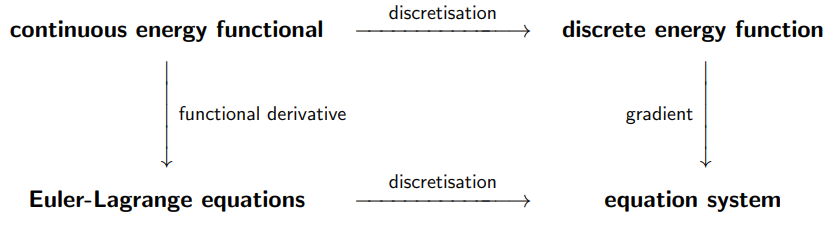
\includegraphics[scale=0.5]{assets/strategies.png}
  \begin{itemize}
    \item Optimise-then-Discretise
    \item Discretise-then-Optimise
  \end{itemize}
  Often the latter is favoured, since it allows automatic handling of boundary conditions.
\end{center}
\subsection{Nonquadratic Variational Methods}
So far the methods talked until now, we blurred edges. So we modify the smoothness term $|\nabla u |^2$ so that large gradients are less penalised than before. So we replace $|\nabla u|^2$ with the following function

\[\psi(|\nabla u|^2) := 2\lambda^2 \sqrt{1+|\nabla u|^2 / \lambda ^2}\]
The discretisation gives us nonlinear systems of equations, which are harder to solve.


\subsubsection{From Variational Denoising to Image Compression}
Instead of minimising
\[E_f(u) = \frac{1}{2}\int_\Omega \left((u-f)^2 + \alpha |\nabla u|^2\right) dx dy\]
we replace $\frac{1-c}{c} := \alpha$ so, $c=\frac{1}{1+\alpha}$

so we get
\[E_f(u) = \frac{1}{2}\int_\Omega \left(c(u-f)^2 + (1-c) |\nabla u|^2\right) dx dy\]

This yields the Euler-Lagrange equation
\[c(u-f)-(1-c)\Delta u = 0\]
\paragraph{Application to Inpainting and Compression}: We can make $c$ space-variant
\[c(x) := \begin{cases}
  1 \quad x \in K \\
  0 \quad \text{else}
\end{cases}\]
This allows us to use
\[c(x)(u-f) - (1-c(x))\Delta u = 0\]
for interpolation purposes. The interpolated image $u$ is identical to $f$ in K, and it solves the Laplace Equation $\nabla u = 0$ in $\Omega \backslash K$

This fills in missing information in $\Omega \backslash K$. This is called \textbf{Inpainting}. Can be used for image compression if we specify data only at some points, e.g edge contours
\begin{center}
  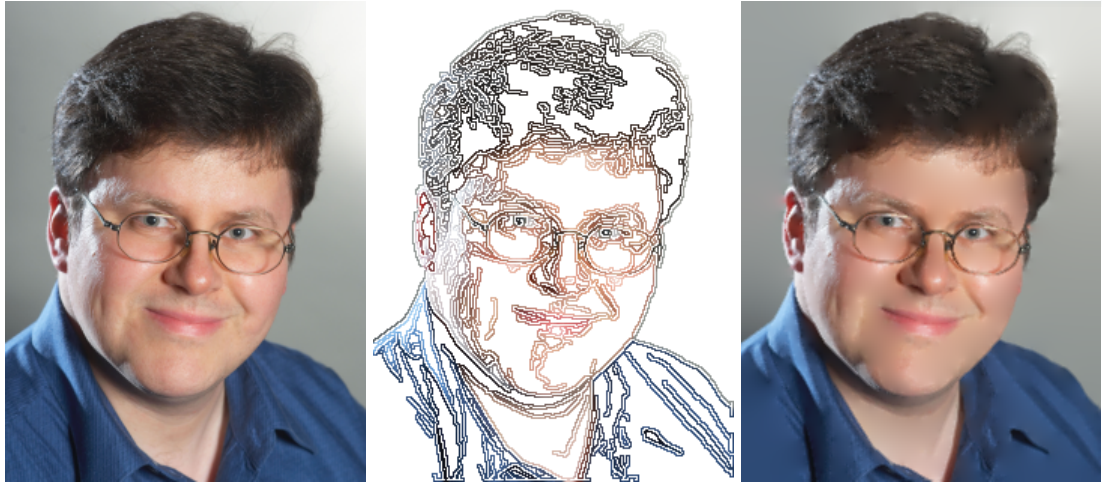
\includegraphics[scale=0.5]{assets/inpainting.png}

  Original vs Edge set vs Interpolation by solving laplace equation
\end{center}
\subsection{Fourier Methods and Deconvolution}
Some types of artifacts (periodic artifacts) are easy to be seen and remove in the Fourier Domain.

\subsubsection{Homomorphic Filtering}
The goal is to restore a picture that has been taken under space-variant illumination conditions

The gray values are the product of illumination intensity and reflectance of the illuminated object.
\[f(x,y) = I(x,y)R(x,y)\]
The reflectance can change rapidly, so it can contain high-frequency components. Illumination intensity is only slowly changing in space, it only contributes low-frequent multiplicative perturbation.

So the idea is to compute the logarithm of all gray values
\[\ln f(x,y) = \ln I(x,y) + \ln R(x,y)\]
Because of this additive superposition, we can now take advantage of the linearity of the fourier transform.

Process
\begin{enumerate}
  \item Compute Fourier Transform $\ln f(x,y)$
  \item Multiply in the Fourier domain with a function that attenuates low frequencies (Illumination intensity) and boosts high frequencies (Reflectance)
  \item Compute inverse Fourier Transform
  \item Compute exponential of result
\end{enumerate}
\begin{center}
  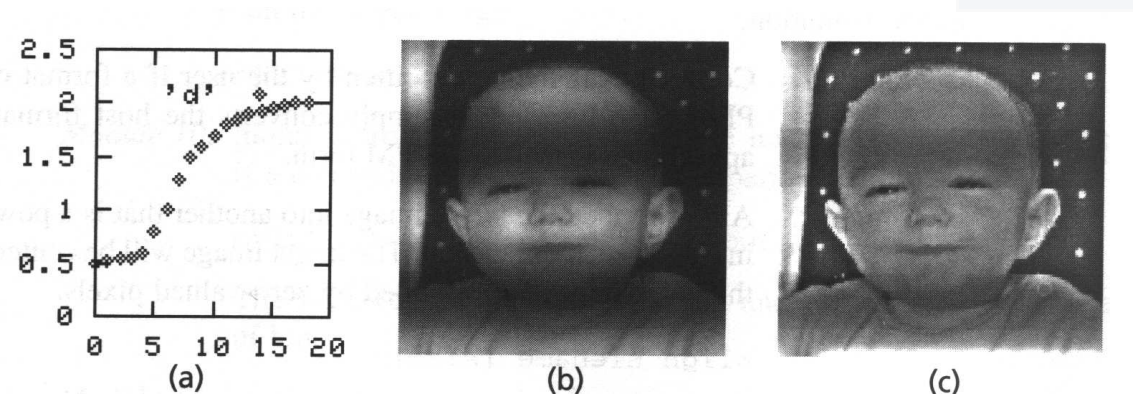
\includegraphics[scale=0.4]{assets/homomorphic_filtering.png}
\end{center}
\subsubsection{Inverse Filtering}
If we remember our Image Degradation model:
\[f(x,y) = (h\ast u )(x,y) + n(x,y)\]
With $u$ being the ideal image, $f$ the degraded version, $h$ the shift-invariant convolution kernel (known), and $n$ the noise.

\paragraph{How can u be restored?} If the noise is negligible, in the Fourier Domain the following stands
\[\hat{f} = \hat{h} \cdot \hat{u}\]
So if $\hat{h}$ does not vanish, we can just compute $u$ from
\[\hat{u} = \frac{\hat{f}}{\hat{h}}\]
and applying the inverse FT

This process is called \textbf{Inverse Filtering}

The issue is that $h$ is usually a smoothing kernel (lowpass filter). So for high frequencies $\hat{h} \approx 0$. In that case, inverse filtering masively amplifies even tiny-high frequent noise.

Without extra stabilisation,  inverse filtering is of basically no use.

The easiest stabilisiation (\textbf{pseudoinverse filtering})
\[\hat{u} = \begin{cases}
  \frac{\hat{f}}{\hat{h}} \quad |\hat{h}| > \varepsilon \\
  0 \quad else
\end{cases}\]
\begin{center}
  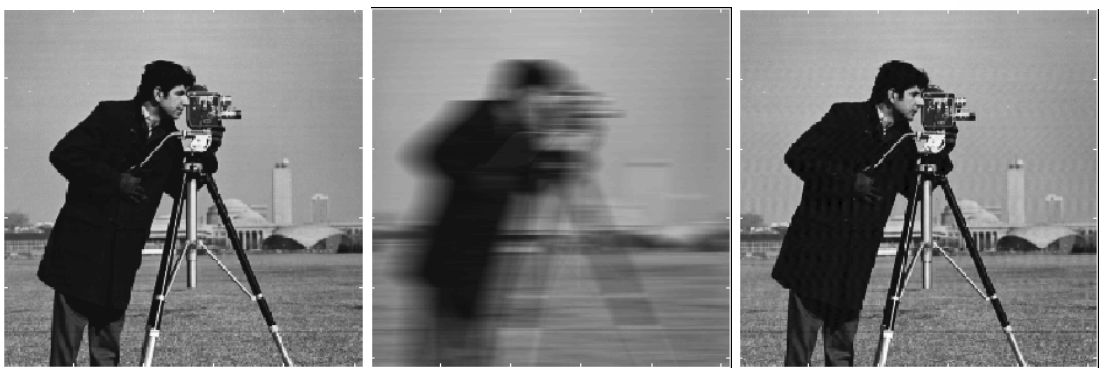
\includegraphics[scale=0.5]{assets/inverse_filtering.png}

  Original vs Simulated motion blur vs Deblurring via pseudoinverse filtering
\end{center}

\subsubsection{Wiener Filtering}
It's a more advanced stabilisiation of the inverse filtering through
\[\hat{u} \approx \frac{1}{\hat{h}}\underbrace{\frac{|\hat{h}|^2}{|\hat{h}|^2  + K}}_{\text{stabilisation}} \hat{f}\]
with positive parameter K. Does not divrge for $\hat{h} \to 0$

Properties
\begin{itemize}
  \item More robust to noise than the simple version
  \item If noise variance is larger, $K$ should be increased
  \item For Gaussian Noise, the optimal K is given by
  \[K := \frac{\sigma^2_{noise}}{\sigma^2_{signal}} = \frac{1}{SNR}\]
  However, these variances not known and usually have to be estimated
\end{itemize}
\subsubsection{Variational Deconvolution Methods}
So far
\[E_f(u) = \frac{1}{2}\int_\Omega ((u-f)^2 + \alpha |\nabla u|^2)dxdy\]
Modifying it by introducing shift-invariant blurring kernel $h$
\[E_f(u) = \frac{1}{2}\int_\Omega ((h \ast u-f)^2 + \alpha |\nabla u|^2)dxdy\]
Giving us the Euler-Lagrange equation
\[0 = h^* \ast(h\ast u - f) - \alpha \Delta u\]
Where $h^*$ is the adjoint blurring kernel $h^*(x,y) = h(-x,-y)$

\subsubsection{Blind Deconvolution}
Often the blurring kernel is unknown, so the question is: is it possible to estimate both $h$ and $u$ at the same time?

We minimise an energy with regularisers for both $u$ and $h$
\[E(u,h) = \frac{1}{2}\int_\Omega ((h\ast u - f)^2 + \alpha |\nabla u|^2 + \beta |\nabla h|^2)dxdy\]
This creates two coupled Euler-Lagrange equations
\[0 = h^* \ast ( h\ast u - f) - \alpha \Delta u\]
\[0 = u^* \ast ( h\ast u - f) - \alpha \Delta h\]
The discretisation can be computed in an iterative and alternating manner. Suitable initializations are required. You can also use non-quadratic regularisers

\begin{center}
  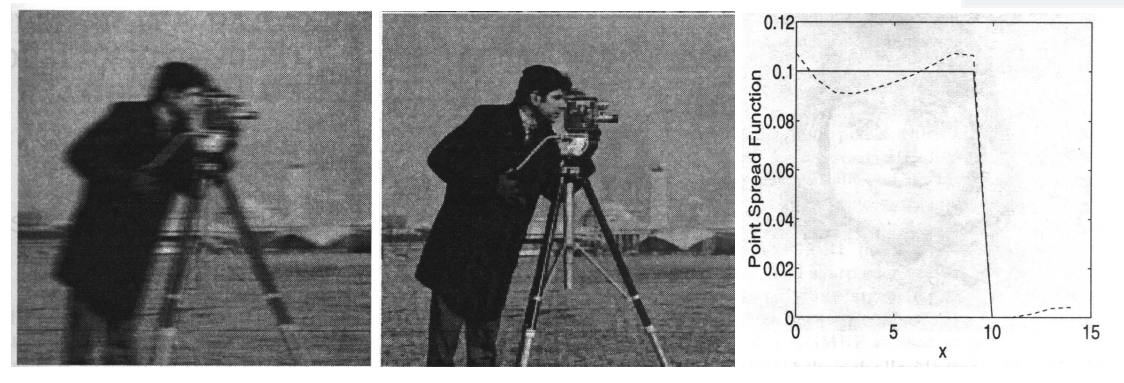
\includegraphics[scale=0.4]{assets/blind_deconvolution.png}

  The rightmost image is the true kernel vs its estimation
\end{center}

And this is it! Very very nice lecture :)
\end{document}





